% ================================================================
% C++ 第七章 指针 —— 基础学习讲义（单文件完整源码）
% 编译：xelatex 编译两次
% 字体：Noto Serif CJK / Noto Sans CJK（.ttc，使用索引 2 = 简体中文）、DejaVu Sans、DejaVu Sans Mono
% ================================================================
% ================================================================
%  C++ 第七章 指针 —— 基础学习讲义   导言区
%  编译方式：XeLaTeX（两次）
% ================================================================
\documentclass[UTF8,a4paper,11pt,fontset=none,zihao=-4]{ctexart}

% ---------- 字体 ----------
% Noto CJK 为字体集合（.ttc），索引 2 才是简体中文（SC）字形；按名称选取可能落到日文（JP）字形
\setCJKmainfont{NotoSerifCJK-Regular.ttc}[FontIndex=2,BoldFont=NotoSansCJK-Bold.ttc,BoldFeatures={FontIndex=2},
  ItalicFont=NotoSerifCJK-Regular.ttc,ItalicFeatures={FontIndex=2,FakeSlant=0.15}]
\setCJKsansfont{NotoSansCJK-Regular.ttc}[FontIndex=2,BoldFont=NotoSansCJK-Bold.ttc,BoldFeatures={FontIndex=2}]
\setCJKmonofont{NotoSansCJK-Regular.ttc}[FontIndex=2]
\setCJKfamilyfont{hei}{NotoSansCJK-Regular.ttc}[FontIndex=2,BoldFont=NotoSansCJK-Bold.ttc,BoldFeatures={FontIndex=2}]
\newcommand{\hei}{\CJKfamily{hei}}
\setmonofont{DejaVu Sans Mono}[Scale=0.88]
\newfontfamily\circfont{DejaVu Sans}[Scale=0.92]
\newcommand{\ci}[1]{{\circfont #1}}

% ---------- 版面 ----------
\usepackage[a4paper,top=22mm,bottom=22mm,left=21mm,right=21mm,headsep=6mm,headheight=24pt,footskip=10mm]{geometry}
\linespread{1.32}
\setlength{\parskip}{3pt plus 1pt}
\usepackage{microtype}

% ---------- 数学 / 表格 / 列表 ----------
\usepackage{amsmath,amssymb,mathtools,bm}
\usepackage{booktabs,tabularx,longtable,array,multirow}
\renewcommand{\arraystretch}{1.12}
\newcolumntype{H}[1]{>{\leavevmode\sffamily\bfseries\color{mainc}\raggedright\arraybackslash}p{#1}}
\newcolumntype{A}[1]{>{\leavevmode\small\color{auxc}\raggedright\arraybackslash}p{#1}}
\newcolumntype{Y}{>{\raggedright\arraybackslash}X}
\usepackage{enumitem}
\setlist{itemsep=1pt,topsep=3pt,parsep=0pt,leftmargin=2em}
\usepackage{pifont}
\newcommand{\cmark}{\textcolor{okc}{\ding{51}}}
\newcommand{\xmark}{\textcolor{badc}{\ding{55}}}
\usepackage{needspace}
\usepackage{float}
\usepackage{caption}
\captionsetup{font={small,sf},labelfont={bf,color=mainc},skip=4pt}

% ---------- 颜色（语义固定） ----------
\usepackage[table]{xcolor}
\definecolor{mainc}{HTML}{173A63}   % 深海军蓝：核心知识
\definecolor{auxc}{HTML}{557A9E}    % 辅助蓝
\definecolor{lightc}{HTML}{F3F6F9}  % 极浅蓝灰：定义底色
\definecolor{formc}{HTML}{E8EFF6}   % 浅蓝：核心公式
\definecolor{warmc}{HTML}{FAF8F4}   % 暖米白：示例 / 历史 / 科普
\definecolor{warmline}{HTML}{C9B99A}
\definecolor{redbg}{HTML}{FFF5F4}   % 极浅红：易错 / 纠错
\definecolor{badc}{HTML}{B03A2E}    % 错误标记
\definecolor{greenbg}{HTML}{F4F8F5} % 极浅绿：总结 / 自检
\definecolor{okc}{HTML}{2E7D4F}     % 正确标记
\definecolor{violetbg}{HTML}{F4F3F8}% 极浅灰紫：跨学科
\definecolor{violetc}{HTML}{6B6891}
\definecolor{beigec}{HTML}{8A7A5C}  % 提升层标签
\definecolor{gridc}{HTML}{C8D3DE}
\definecolor{codebg}{HTML}{F7F8FA}
\definecolor{hlc}{HTML}{FCE9C8}     % 图中高亮（淡琥珀）

% ---------- 超链接 ----------
\usepackage[colorlinks=true,linkcolor=mainc,urlcolor=auxc,citecolor=mainc,
  bookmarksnumbered=true,pdftitle={C++ 指针：基础学习讲义},pdfauthor={课程讲义整理}]{hyperref}

% ---------- TikZ / PGFPlots ----------
\usepackage{tikz}
\usetikzlibrary{arrows.meta,positioning,calc,fit,backgrounds,shapes.misc,decorations.pathreplacing,shapes.geometric,matrix}
\usepackage{pgfplots}
\pgfplotsset{compat=1.18}
\usepackage{forest}

% ---------- 页眉页脚 ----------
\usepackage{fancyhdr}
\pagestyle{fancy}
\fancyhf{}
\fancyhead[L]{\small\sffamily\color{auxc}C++ 第七章\enspace 指针 · 基础学习讲义}
\fancyhead[R]{\small\sffamily\color{auxc}\leftmark}
\fancyfoot[C]{\small\sffamily\color{mainc}\thepage}
\renewcommand{\headrulewidth}{0.4pt}
\renewcommand{\headrule}{\hbox to\headwidth{\color{gridc}\leaders\hrule height \headrulewidth\hfill}}

% ---------- 标题样式 ----------
\ctexset{
  section={name={第,讲},number=\chinese{section},
    format=\color{mainc}\Large\bfseries\sffamily\raggedright,
    beforeskip=16pt plus 4pt,afterskip=8pt,aftername=\quad},
  subsection={format=\color{mainc}\large\bfseries\sffamily\raggedright,
    beforeskip=11pt plus 3pt,afterskip=5pt},
  subsubsection={format=\color{auxc}\normalsize\bfseries\sffamily\raggedright,
    beforeskip=7pt plus 2pt,afterskip=3pt},
  paragraph={format=\color{mainc}\bfseries\sffamily,runin=true,afterskip=0.6em},
  contentsname={目\quad 录}
}
\renewcommand{\sectionmark}[1]{\markboth{#1}{}}
\setcounter{secnumdepth}{2}
\setcounter{tocdepth}{1}
% 不编号的大模块（导读、练习、解析）也进入目录和页眉
\newcommand{\usection}[1]{\needspace{14\baselineskip}\section*{#1}\addcontentsline{toc}{section}{#1}\markboth{#1}{}}
\newcommand{\usubsection}[1]{\subsection*{#1}\addcontentsline{toc}{subsection}{#1}}

% ---------- tcolorbox 统一信息框体系 ----------
\usepackage[most]{tcolorbox}
\tcbset{
  basebox/.style={enhanced,breakable,arc=2pt,boxrule=0.5pt,left=7pt,right=7pt,top=9pt,bottom=5pt,
    fonttitle=\sffamily\bfseries\small,before skip=7pt,after skip=7pt,
    coltitle=white,attach boxed title to top left={xshift=6pt,yshift*=-\tcboxedtitleheight/2},
    boxed title style={arc=1.5pt,boxrule=0pt}},
  sidebox/.style={enhanced,breakable,frame hidden,sharp corners,borderline west={2.2pt}{0pt}{#1},
    left=9pt,right=6pt,top=4pt,bottom=4pt,before skip=7pt,after skip=7pt,
    fonttitle=\sffamily\bfseries\small,coltitle=#1,detach title,
    before upper={\tcbtitle\par\smallskip}},
}
% 一级知识块
\newtcolorbox{definitionbox}[1][]{basebox,colback=lightc,colframe=mainc,
  boxed title style={colback=mainc},title={定义\ifx\relax#1\relax\else{}：#1\fi}}
\newtcolorbox{formulabox}[1][]{basebox,colback=formc,colframe=mainc,
  boxed title style={colback=mainc},title={核心关系\ifx\relax#1\relax\else{}：#1\fi}}
\newtcolorbox{theorembox}[1][]{basebox,colback=lightc,colframe=mainc,
  boxed title style={colback=mainc},title={结论\ifx\relax#1\relax\else{}：#1\fi}}
% 二级知识块（左侧色条）
\newtcolorbox{intuitionbox}[1][为什么 / 直观理解]{sidebox=auxc,colback=lightc,title={#1}}
\newtcolorbox{proofbox}[1][证明 / 推导]{sidebox=mainc,colback=white,title={#1},
  after upper={\unskip\nobreak\hfill\textcolor{mainc}{$\blacksquare$}}}
\newtcolorbox{supplementbox}[1][]{sidebox=auxc,colback=lightc,
  title={教学补全\ifx\relax#1\relax\else{}：#1\fi},
  before upper={\tcbtitle\par{\footnotesize\color{auxc}原始笔记未完整展示该部分，以下按照本课程常见教材与 C++ 标准表述补充。}\par\smallskip}}
\newtcolorbox{connectionbox}[1][学科联系]{sidebox=auxc,colback=lightc,title={#1}}
\newtcolorbox{extendbox}{sidebox=auxc!70,colback=white,title={拓展联想},
  before upper={\tcbtitle\par{\footnotesize\color{auxc}以下内容只用于建立知识联系，当前阶段不要求掌握。}\par\smallskip}}
% 示例 / 历史 / 科普（暖米白）
\newtcolorbox{examplebox}[1][]{basebox,colback=warmc,colframe=warmline,
  boxed title style={colback=beigec},title={例题\ifx\relax#1\relax\else\enspace#1\fi}}
\newtcolorbox{historybox}[1][]{sidebox=beigec,colback=warmc,title={#1}}
\newtcolorbox{sciencebox}[1][]{sidebox=beigec,colback=warmc,title={#1}}
% 易错 / 纠错（极浅红）
\newtcolorbox{warningbox}[1][易错点]{sidebox=badc,colback=redbg,title={#1}}
\newtcolorbox{correctionbox}[1]{basebox,colback=redbg,colframe=badc!60,
  boxed title style={colback=badc!85},title={原图纠错 · #1}}
% 总结 / 自检（极浅绿）
\newtcolorbox{summarybox}[1][方法总结]{sidebox=okc,colback=greenbg,title={#1}}
\newtcolorbox{checkbox}[1][学完这里，你应该能够回答]{sidebox=okc,colback=greenbg,title={#1}}
% 三级提示：细色线 + 普通正文
\newcommand{\tip}[2][注意]{\par\noindent{\color{auxc}\rule[-0.3ex]{1.5pt}{2.3ex}}\enspace{\sffamily\bfseries\color{auxc}#1}\enspace #2\par}

% ---------- 代码 ----------
\usepackage{listings}
\lstdefinestyle{cpp}{language=C++,basicstyle=\ttfamily\small,
  keywordstyle=\color{mainc}\bfseries,commentstyle=\color{okc!80!black},
  stringstyle=\color{beigec!80!black},numberstyle=\tiny\color{auxc},
  numbers=left,numbersep=6pt,xleftmargin=16pt,columns=fullflexible,keepspaces=true,
  showstringspaces=false,tabsize=4,breaklines=true,
  morekeywords={nullptr,NULL,sizeof,const,using,namespace},
  literate={＝}{{=}}1}
\lstset{style=cpp}
\tcbset{codestyle/.style={enhanced,breakable,listing only,colback=codebg,colframe=gridc,boxrule=0.4pt,arc=2pt,
  left=2pt,right=4pt,top=1pt,bottom=1pt,before skip=5pt,after skip=5pt}}
\newtcblisting{code}{codestyle,listing options={style=cpp}}
\newtcblisting{codeout}{codestyle,colback=white,listing options={style=cpp,numbers=none,xleftmargin=4pt,keywordstyle=,stringstyle=,commentstyle=}}
\newcommand{\cpp}[1]{\lstinline[style=cpp,basicstyle=\ttfamily,numbers=none]{#1}}
\newcommand{\cc}[1]{\texttt{#1}}

% ---------- 通用 TikZ 样式：内存图 ----------
\tikzset{
  >={Stealth[length=2.2mm]},
  cell/.style={draw=mainc,line width=0.6pt,fill=white,minimum width=15mm,minimum height=7mm,inner sep=1pt,font=\ttfamily\small},
  pcell/.style={cell,fill=formc},
  scell/.style={cell,minimum width=10mm},
  acell/.style={draw=mainc,line width=0.6pt,fill=white,minimum width=9mm,minimum height=7mm,inner sep=0pt,font=\ttfamily\small},
  hl/.style={fill=hlc},
  badcell/.style={draw=badc,fill=redbg},
  vn/.style={font=\ttfamily\small\bfseries,text=mainc,anchor=east,inner sep=2pt},
  ad/.style={font=\ttfamily\scriptsize,text=auxc,anchor=south,inner sep=1.2pt},
  adt/.style={ad,font=\ttfamily\fontsize{5.5}{6}\selectfont},
  idx/.style={font=\ttfamily\scriptsize,text=auxc,anchor=north,inner sep=1.2pt},
  ptr/.style={->,line width=0.9pt,draw=mainc},
  ptrbad/.style={->,line width=0.9pt,draw=badc,dashed},
  ptrok/.style={->,line width=0.9pt,draw=okc},
  note/.style={font=\sffamily\footnotesize,text=auxc,align=center},
  bnote/.style={font=\sffamily\footnotesize,text=badc,align=center},
  gnote/.style={font=\sffamily\footnotesize,text=okc,align=center},
  frame/.style={draw=gridc,rounded corners=2pt,line width=0.5pt},
  lock/.pic={\fill[badc] (-0.11,-0.1) rectangle (0.11,0.06);
             \draw[badc,line width=0.9pt] (-0.07,0.06) -- (-0.07,0.11) arc (180:0:0.07) -- (0.07,0.06);},
  forbid/.pic={\draw[badc,line width=1.2pt] (-0.15,-0.15) -- (0.15,0.15) (-0.15,0.15) -- (0.15,-0.15);},
}
% \cell[样式]{id}{坐标}{变量名}{值}
\newcommand{\cell}[5][]{\node[cell,#1] (#2) at (#3) {#5};\node[vn] at (#2.west) {#4};}
% \pcell[样式]{id}{坐标}{变量名}{值}  —— 指针变量（浅蓝底）
\newcommand{\pcell}[5][]{\node[pcell,#1] (#2) at (#3) {#5};\node[vn] at (#2.west) {#4};}
% \addr{id}{地址文字}
\newcommand{\addr}[2]{\node[ad] at (#1.north) {#2};}
% \arr[单元样式]{id}{起点坐标}{值列表}{数组名}：连续单元，下标写在下方
\newcommand{\arr}[5][]{%
  \foreach \v [count=\k from 0] in {#4} {\node[acell,#1] (#2-\k) at ($(#3)+(\k*0.9,0)$) {\v};
    \node[idx] at (#2-\k.south) {[\k]};}
  \node[vn] at (#2-0.west) {#5};}
% 统一选项小图面板：\optpanel{A}{tikz 内容}
\newcommand{\optpanel}[2]{\begin{minipage}[t]{0.485\linewidth}\centering
  {\sffamily\bfseries\color{mainc}(#1)}\par\vspace{1pt}
  \begin{tikzpicture}[baseline=(current bounding box.north)]
  \useasboundingbox (-1.4,-1.2) rectangle (5.6,0.65); #2\end{tikzpicture}\end{minipage}}
% 解析区选项：\optsol{A}{1=正确/0=错误}{tikz}{文字}
\newcommand{\optsol}[4]{\begin{minipage}[t]{0.485\linewidth}
  \ifnum#2=1 \colorbox{greenbg}{\sffamily\bfseries\color{okc}(#1)\enspace\ding{51}\ 正确}%
  \else\colorbox{redbg}{\sffamily\bfseries\color{badc}(#1)\enspace\ding{55}\ 错误}\fi\par\vspace{1pt}
  \centering\begin{tikzpicture}[baseline=(current bounding box.north)]
  \useasboundingbox (-1.4,-1.2) rectangle (5.6,0.65); #3\end{tikzpicture}\par
  \raggedright\small\noindent #4\end{minipage}}

% ---------- 练习与解析 ----------
\newcounter{exq}
\newcommand{\lvtag}[1]{%
  \ifcase#1\or\colorbox{lightc}{\color{auxc}\sffamily\scriptsize\bfseries 基础}%
  \or\colorbox{warmc}{\color{beigec}\sffamily\scriptsize\bfseries 提升}%
  \or\colorbox{violetbg}{\color{violetc}\sffamily\scriptsize\bfseries 跨学科}\fi}
% \q{层级 1/2/3}{知识点}  —— 题号自动递增
\newcommand{\q}[2]{\par\needspace{9\baselineskip}\medskip\refstepcounter{exq}\noindent
  {\sffamily\bfseries\color{mainc}\theexq.}\enspace\lvtag{#1}\enspace{\scriptsize\color{auxc}\sffamily #2}\par\nopagebreak}
\newcommand{\choices}[4]{\par\nopagebreak\noindent\begin{tabularx}{\linewidth}{@{}YY@{}}(A)\ #1 & (B)\ #2\\ (C)\ #3 & (D)\ #4\end{tabularx}\par}
\newcommand{\blank}[1][2.2cm]{\underline{\hspace{#1}}}
% 解析标题：\sol{题号}{答案}{难度}{知识点}
\newcommand{\sol}[4]{\par\needspace{6\baselineskip}\medskip
  \noindent\begin{tcolorbox}[enhanced,colback=lightc,colframe=lightc,arc=1.5pt,left=5pt,right=5pt,top=2pt,bottom=2pt,before skip=6pt,after skip=4pt]
  {\sffamily\bfseries\color{mainc}第 #1 题}\quad\lvtag{#3}\quad{\sffamily\small 答案：\textbf{\color{okc}#2}}\hfill{\scriptsize\sffamily\color{auxc}考点：#4}\end{tcolorbox}\nopagebreak}
\newcommand{\step}[1]{\par\noindent{\sffamily\bfseries\color{auxc}#1}\enspace}
\newcommand{\oneline}[1]{\par\noindent{\color{okc}\sffamily\bfseries 一句话总结}\enspace#1\par}

% 常用图形尺寸
\newcommand{\figcap}[1]{\par\vspace{2pt}{\centering\small\sffamily\color{auxc}#1\par}\vspace{2pt}}
% \arrx{id}{起点}{值列表}{左侧标签}{从该下标起标绿(已就位)}{高亮下标1}{高亮下标2}
\newcommand{\arrx}[7]{%
  \foreach \v [count=\k from 0] in {#3} {
    \tikzset{cst/.style={fill=white}}%
    \ifnum\k>\numexpr#5-1\relax \tikzset{cst/.style={fill=greenbg,draw=okc}}\fi
    \ifnum\k=#6 \tikzset{cst/.style={fill=hlc}}\fi
    \ifnum\k=#7 \tikzset{cst/.style={fill=hlc}}\fi
    \node[acell,cst] (#1-\k) at ($(#2)+(\k*0.9,0)$) {\v};}
  \node[vn,font=\sffamily\scriptsize\bfseries] at (#1-0.west) {#4};}

\begin{document}
% ================================================================
%  封面 · 阅读说明 · 目录 · 导读 · 学科小史 · 科普 · 原始资料重编码与纠错
% ================================================================
\begin{titlepage}
\thispagestyle{empty}
\begin{tikzpicture}[remember picture,overlay]
  \fill[mainc] (current page.north west) rectangle ([yshift=-9mm]current page.north east);
  \fill[auxc] ([yshift=-9mm]current page.north west) rectangle ([yshift=-10.2mm]current page.north east);
  \fill[lightc] (current page.south west) rectangle ([yshift=16mm]current page.south east);
\end{tikzpicture}
\vspace*{22mm}

{\sffamily\color{auxc}\large C++ 程序设计\enspace{}·\enspace{}第七章}\par\vspace{6mm}
{\sffamily\bfseries\color{mainc}\fontsize{40}{48}\selectfont 指\ 针}\par\vspace{5mm}
{\sffamily\color{mainc}\Large 从“内存地址”到“用指针排序数组”}\par\vspace{2mm}
{\color{auxc}\rule{0.62\linewidth}{0.8pt}}\par\vspace{3mm}
{\sffamily\large\color{mainc}基础学习讲义}\enspace{\sffamily\color{auxc}可视化图解 · 推导补全 · 分层练习}\par
\vspace{16mm}

\begin{center}
\begin{tikzpicture}[scale=1]
  % 内存条
  \foreach \i/\v/\a in {0/{},1/{10},2/{},3/{},4/{0x1004},5/{},6/{}} {
    \node[cell,minimum width=18mm,minimum height=9mm] (m\i) at (\i*1.8,0) {\v};
  }
  \node[ad,font=\ttfamily\footnotesize] at (m1.north) {0x1004};
  \node[ad,font=\ttfamily\footnotesize] at (m4.north) {0x2010};
  \node[font=\ttfamily\bfseries\color{mainc}] at ([yshift=-5mm]m1.south) {int a};
  \node[font=\ttfamily\bfseries\color{mainc}] at ([yshift=-5mm]m4.south) {int *p};
  \node[pcell,minimum width=18mm,minimum height=9mm] at (m4) {0x1004};
  \node[cell,minimum width=18mm,minimum height=9mm,hl] at (m1) {10};
  \draw[ptr,line width=1.3pt] ([yshift=4mm]m4.north) to[out=140,in=40] node[above,note,font=\sffamily\small]{p 保存的是 a 的地址} ([yshift=4mm]m1.north);
  \node[note] at ([xshift=-12mm]m0.west) {$\cdots$};
  \node[note] at ([xshift=12mm]m6.east) {$\cdots$};
  \draw[decorate,decoration={brace,amplitude=4pt,mirror},draw=auxc] ([yshift=-9mm]m0.south west) -- ([yshift=-9mm]m6.south east)
    node[midway,below=5pt,note]{内存：一排按地址编号的存储单元};
\end{tikzpicture}
\end{center}
\vspace{14mm}

\noindent\begin{tabularx}{\linewidth}{@{}A{2.4cm}X@{}}
\toprule
适用对象 & 第一次学习 C++ 指针、前置基础不太牢固的本科生 \\
原始依据 & 课堂手写笔记 11 页（§7.1～§7.8：基本概念、定义与使用、所占空间、空指针与野指针、const 修饰指针、指针和数组、指针和函数、指针+数组+函数综合案例） \\
本讲义做了什么 & 识别重编码 $\to$ 纠正笔记中的 6 处问题 $\to$ 补全推导与证明 $\to$ 内存图解 $\to$ 38 道分层练习与逐选项图解 \\
编译环境 & XeLaTeX；全部示例代码已用 g++（C++17，64 位 Linux）实际编译运行 \\
\bottomrule
\end{tabularx}
\end{titlepage}

% ---------------- 阅读说明 ----------------
\usection{阅读说明}
这份讲义不是把笔记“抄一遍”，而是把笔记里讲到的每一个知识点，按照“先知道为什么、再建立图像、然后给定义和公式、最后练习”的顺序重新讲一遍。建议这样使用：

\noindent\begin{tabularx}{\linewidth}{@{}H{2.3cm}X@{}}
\toprule
第一次学习 & 按顺序读第一讲～第八讲，每讲末尾的“自检”能答出来再往后走。遇到内存图，先用手指沿着箭头“走一遍”。\\
课前预习 & 只读每讲开头的“本讲回答的问题”和“直观理解”框，建立印象即可。\\
课后复习 & 重点看“易错点”（浅红色框）和“相近概念辨析”表格，再做 A 组基础题。\\
考前巩固 & 直接做练习 A、B、C 三组，对照答案速查，错题再回到对应讲次（见“知识点—题目对应表”）。\\
\bottomrule
\end{tabularx}

\paragraph{颜色约定} 全书颜色含义固定，读几页之后就能“看颜色知用途”：

\noindent
\begin{tikzpicture}
\foreach \c/\t/\x in {lightc/定义·核心知识/0, formc/核心关系式/3.05, warmc/例题·历史·科普/6.1, redbg/易错·原图纠错/9.15, greenbg/总结·自检/12.2}{
  \node[draw=gridc,fill=\c,minimum width=28mm,minimum height=7mm,font=\sffamily\footnotesize,rounded corners=1.5pt] at (\x,0) {\t};}
\end{tikzpicture}

\paragraph{内存图约定} 本书所有内存图使用同一套画法，请先认识它们：

\begin{center}
\begin{tikzpicture}
  \cell{a}{0,0}{a}{10}\addr{a}{0x1000}
  \pcell{p}{5,0}{p}{0x1000}\addr{p}{0x2000}
  \draw[ptr] (p.south) to[out=-150,in=-30] (a.south);
  \node[note,anchor=west] at (7,0.35) {白底方框：普通变量（框内是值）};
  \node[note,anchor=west] at (7,-0.2) {浅蓝方框：指针变量（框内是地址）};
  \node[note,anchor=west] at (7,-0.75) {框上方小字：该变量自己的地址};
  \node[note,anchor=west] at (7,-1.3) {深蓝箭头：“指向”关系};
  \pic at (0,-1.4) {lock}; \node[note,anchor=west] at (0.2,-1.4) {红锁：不可修改（const）};
  \draw[ptrbad] (3.2,-2) -- (4.4,-2); \node[note,anchor=west] at (4.5,-2) {红虚线箭头：非法 / 危险的指向};
\end{tikzpicture}
\end{center}

\tip[提示]{图中的地址（如 \cc{0x1000}）都是为了讲解而选的“好看的数”。真实程序每次运行打印出的地址一般不同，且通常很长（如 \cc{0x7ffcc6ee782c}）。}

\clearpage\tableofcontents
\clearpage

% ================================================================
\usection{导读：本专题学什么、在哪里、需要什么}
% ================================================================
\subsection*{本专题回答的核心问题}
学到第七章之前，我们一直在用“变量名”操作数据：\cpp{a = 10;}、\cpp{cout << a;}。这很方便，但留下了几个解决不了的问题：

\begin{enumerate}[label=\arabic*.]
  \item 一个函数想\textbf{修改调用者的变量}（比如交换两个数），只拿到“值的副本”是做不到的；
  \item 把一个很大的数组交给函数处理时，我们不希望把整个数组复制一份，只想告诉函数\textbf{“数据在哪儿”}；
  \item 有些数据根本没有名字，只有位置（例如以后学的动态内存、硬件寄存器），只能按\textbf{地址}访问。
\end{enumerate}
这三个问题的共同答案就是：\textbf{把“地址”本身也当成一种数据，存起来、传出去、用它间接访问内存}。存放地址的变量就叫\textbf{指针}。

\subsection*{本专题在课程体系中的位置}
\begin{center}
\begin{tikzpicture}[
  box/.style={draw=mainc,fill=lightc,rounded corners=2pt,minimum height=8mm,font=\sffamily\small,align=center,inner xsep=4pt},
  cur/.style={box,fill=mainc,text=white,font=\sffamily\small\bfseries},
  fut/.style={box,fill=white,draw=auxc,text=auxc},
  lk/.style={->,draw=auxc,line width=0.7pt}]
  \node[box] (var) at (0,1.45) {变量与数据类型\\(第2章)};
  \node[box] (arr) at (0,0) {数组\\(第5章)};
  \node[box] (fun) at (0,-1.45) {函数与参数传递\\(第6章)};
  \node[cur,minimum width=30mm,minimum height=16mm] (ptr) at (4.4,0) {第7章\\指针};
  \node[fut] (ref) at (8.9,1.6) {引用 \& 结构体};
  \node[fut] (dyn) at (8.9,0.55) {动态内存 new/delete};
  \node[fut] (ds) at (8.9,-0.5) {数据结构：链表/树};
  \node[fut] (os) at (8.9,-1.55) {操作系统 · 嵌入式};
  \foreach \s in {var,arr,fun} \draw[lk] (\s.east) -- (ptr.west);
  \foreach \t in {ref,dyn,ds,os} \draw[lk] (ptr.east) -- (\t.west);
  \node[note] at (0,2.5) {前置知识}; \node[note] at (8.9,2.4) {后续知识};
\end{tikzpicture}
\end{center}

\subsection*{前置知识地图：开始之前你需要知道的五件事}
\noindent\begin{tabularx}{\linewidth}{@{}H{2.6cm}XA{3.3cm}@{}}
\toprule
前置知识 & 本章要用到的最少内容 & 用在哪里 \\
\midrule
变量与类型 & \cc{int a = 10;} 会在内存中划出一块空间（\cc{int} 一般 4 字节）并存入 10 & 第一讲、第二讲 \\
\cc{sizeof} & \cc{sizeof(x)} 给出 \cc{x} 占用的字节数，编译时就已确定 & 第三讲、第八讲 \\
数组 & \cc{int arr[5]} 是 5 个 \cc{int} \textbf{紧挨着}存放；下标从 0 开始，合法范围 \cc{0～4} & 第六讲、第八讲 \\
函数 & 调用 \cc{f(a)} 时，形参是实参的\textbf{拷贝}（值传递） & 第七讲 \\
十六进制 & \cc{0x} 开头表示十六进制：\cc{0x10}$=16$，\cc{0x0C}$=12$ & 全章地址计算 \\
\bottomrule
\end{tabularx}

\begin{supplementbox}[十六进制快速复习]
十六进制每一位取 \cc{0～9, A～F}（A=10，…，F=15），第 $k$ 位（从右往左、从 0 数）的权是 $16^k$。例如
\[
\texttt{0x0010}=1\times16^1+0=16,\qquad \texttt{0x100C}=1\times16^3+0+0+12=4108 .
\]
地址习惯用十六进制书写，原因是一位十六进制恰好对应 4 个二进制位，两位恰好是 1 个字节，和计算机“按字节编址”的方式对得很整齐。计算地址时最常见的操作是“加几个字节”，例如 $\texttt{0x1000}+12=\texttt{0x100C}$（因为十进制 12 就是十六进制 C）。
\end{supplementbox}

% ================================================================
\usection{学科小史：指针是怎样出现的？}
% ================================================================
今天我们觉得“变量有地址”是理所当然的，但在高级语言发展早期，这是一个需要取舍的设计问题：\textbf{语言应该把机器的“地址”暴露给程序员，还是把它藏起来？}

汇编语言里程序员直接写地址，效率高但极易出错；许多早期高级语言则把地址藏起来，安全但难以编写操作系统这类需要直接操纵内存的程序。指针正是在“既要像汇编一样高效，又要像高级语言一样可读”的需求下成熟起来的。

\begin{center}
\begin{tikzpicture}[scale=0.94,
  ev/.style={font=\sffamily\footnotesize,align=center,text width=26mm},
  yr/.style={font=\sffamily\bfseries\small,text=mainc}]
  \draw[line width=1.2pt,draw=auxc,->] (0,0) -- (15.6,0);
  \foreach \x in {0.9,3.9,6.9,9.9,12.9,15.0} \fill[mainc] (\x,0) circle (2.3pt);
  \node[yr,below=3pt] at (0.9,0) {1965};
  \node[yr,above=3pt] at (3.9,0) {1960s 后期};
  \node[yr,below=3pt] at (6.9,0) {1969--1970};
  \node[yr,above=3pt] at (9.9,0) {1969--1973};
  \node[yr,below=3pt] at (12.9,0) {1979--1985};
  \node[yr,above=3pt] at (15.0,0) {2011};
  \node[ev,above=17pt] at (0.9,0) {ALGOL W 引入“空引用”（Hoare 后称其为“十亿美元的错误”）};
  \node[ev,below=17pt] at (3.9,0) {BCPL（M.~Richards）：地址可以作为数值参与运算};
  \node[ev,above=17pt] at (6.9,0) {B 语言（K.~Thompson）：继承 BCPL 的指针思想};
  \node[ev,below=17pt] at (9.9,0) {C 语言（D.~Ritchie）：带类型的指针，数组名转为指针};
  \node[ev,above=17pt] at (12.9,0) {C with Classes $\to$ C++（B.~Stroustrup）};
  \node[ev,below=17pt] at (15.0,0) {C++11 引入 \texttt{nullptr}};
\end{tikzpicture}
\end{center}

\begin{historybox}[几个真正影响你今天写代码的节点]
\begin{itemize}
  \item \textbf{BCPL 与 B（1960 年代后期—1970 年）}：Martin Richards 设计的 BCPL 和 Ken Thompson 在它基础上做的 B 语言，都允许把地址当作数来运算。但它们只有“机器字”一种数据，指针加 1 就是“下一个字”，没有“类型”的概念。
  \item \textbf{C 语言（1969—1973，贝尔实验室）}：Dennis Ritchie 在 B 的基础上加入了 \cpp{int}、\cpp{char} 等类型，指针也随之有了类型——\cpp{int*} 加 1 前进一个 \cpp{int} 的字节数，\cpp{char*} 加 1 前进 1 个字节。Ritchie 在回顾文章中特别提到，“数组名在表达式中转换为指向首元素的指针”这一规则，是从 B 平滑过渡到 C 的关键设计。这正是本讲义第六讲的核心。
  \item \textbf{C++（1979 年起）}：Bjarne Stroustrup 从 1979 年开始在 C 上增加类，最初叫 “C with Classes”，1983 年改名 C++，1985 年对外发布。C++ 完整保留了 C 的指针，所以本章内容在 C 和 C++ 中几乎一致。
  \item \textbf{空指针的反思}：Tony Hoare 在 2009 年的一次演讲中回顾，他在 1965 年设计 ALGOL W 时引入了“空引用”，并称之为自己的“十亿美元的错误”——因为它引发了无数程序崩溃。C++11 引入更安全的 \cpp{nullptr}，现代语言则进一步从类型系统上限制空值。这正是第四讲“空指针不可访问”背后的历史教训。
\end{itemize}
\end{historybox}
\noindent 读完这段历史，你会发现：\textbf{指针的“类型”决定步长、数组名会变成指针、空指针不能解引用}——这三条今天考试最爱考的规则，都是语言设计者当年有意做出的选择。

% ================================================================
\usection{从课本到现实：指针到底有什么用？}
% ================================================================
\begin{sciencebox}[1. 操作系统：你见过的“段错误”是怎么来的]
笔记里写“空指针访问 $\to$ segmentation fault（段错误）”。这背后是操作系统的\textbf{内存保护}：每个程序只能访问操作系统分配给它的那部分地址；主流操作系统通常故意不把地址 0 附近的区域分配给程序。当程序通过空指针访问地址 0 时，硬件发现“这个地址不属于你”，操作系统就把程序终止，并报告段错误。所以段错误其实是一种\textbf{保护}：宁可让程序立刻崩溃，也不让它悄悄改坏别人的数据。
\end{sciencebox}

\begin{sciencebox}[2. 嵌入式：用指针“按地址”点亮一盏灯]
在单片机里，控制 LED、电机的“寄存器”被安排在固定地址上（由芯片手册规定）。程序员把这个地址强制转换成指针，然后 \cpp{*reg = 1;} 就能让引脚输出高电平。这和笔记里 \cpp{int *p = (int*)0x0010;} 的写法\textbf{形式完全相同}——区别只在于：单片机上这个地址是芯片手册保证可以访问的，而在电脑上随便写的地址不是你的，就成了野指针。（C 组第 37 题就考这个。）
\end{sciencebox}

\begin{sciencebox}[3. 图像与数据：一张照片就是一个很长的数组]
一张 $1920\times1080$ 的灰度图片，在内存中通常就是 $1920\times1080$ 个字节\textbf{按行连续存放}。图像处理程序拿到一个指向首字节的指针，用“指针 + 偏移”走遍每个像素；把图片交给函数处理时，也只传指针和尺寸，而不复制几兆字节的数据——这就是第八讲“数组作函数参数时只传首地址”的现实版本。（C 组第 38 题。）
\end{sciencebox}

\begin{sciencebox}[4. 安全：为什么大家越来越重视“内存安全”]
笔记中“数组 5 个元素却循环 10 次”的越界读取，在真实软件里是一类非常常见、危害很大的安全漏洞来源（缓冲区溢出）。这也是近年来越来越多的工程团队重视内存安全、并在部分场景采用带边界检查的容器或内存安全语言的原因。学好指针的\textbf{边界意识}，是写出安全程序的第一步。
\end{sciencebox}

% ================================================================
\usection{原始笔记的识别、重编码与纠错}
% ================================================================
\subsection*{原始资料内容一览}
原始资料为手写笔记照片 11 页（笔记页码 378--393，日期 2026 年 9 月 25--27 日）。按照笔记本身的小节，识别出的结构如下：

\begin{longtable}{@{}H{1.3cm}>{\raggedright\arraybackslash}p{4.2cm}>{\raggedright\arraybackslash}p{9.2cm}@{}}
\toprule
笔记小节 & 标题 & 可靠识别的主要内容 \\
\midrule\endhead
§7.1 & 基本概念 & 作用：通过指针间接访问内存；内存编号从 0 开始，一般用十六进制表示；可以利用指针变量保存地址；图示 \cc{int a = 10}、\cc{p} 中存 \cc{0x0000}（红字：“可以通过指针保存一个地址”）\\
§7.2 & 指针变量的定义与使用 & 语法“数据类型 * 指针变量名”；\cc{int *p; p = \&a;}；输出 \cc{p}；“可以通过解引用的方式来找到指针指向的内存”，\cc{*p}（红字标注“解引用”）\\
§7.3 & 指针所占的内存空间 & 32 位操作系统 4 字节，64 位操作系统 8 字节；示例 \cc{int b = sizeof(p);} \\
§7.4 & 空指针与野指针 & 空指针：指向编号为 0 的空间，用于初始化，不可访问，\cc{int *p = NULL; *p = 100} $\to$ segmentation fault；野指针：指向非法的内存空间，示例 \cc{int *p = (int*)0x0010;}；红字总结：“空指针和野指针都不是我们申请的空间，因此不要访问” \\
§7.5 & const 修饰指针 & 三种情况：const 修饰指针——常量指针（\cc{const int *p}，指向可改、值不可改）；const 修饰常量——指针常量（\cc{int * const p}，指向不可改、值可改）；两者都修饰（\cc{const int * const p}）；图示与示例代码 \\
§7.6 & 指针和数组 & 利用指针访问数组元素；\cc{int *p = arr;}，\cc{p++}（红字：“向后偏移 4 个字节”）；通过指针遍历数组 \\
§7.7 & 指针和函数 & 利用指针作函数参数可以修改实参；回顾值传递 \cc{swap(int a,int b)}；地址传递 \cc{swap\_p(int *p1,int *p2)}，红字“可以改变实参” \\
§7.8 & 指针、数组和函数 & 案例：封装函数，利用冒泡排序实现整型数组升序排序；先在 \cc{main} 中写冒泡排序并解释两层循环边界；再封装 \cc{BubbleSort(int *arr,int n)}、\cc{PrintArray}，在 \cc{main} 中用 \cc{sizeof(arr)/sizeof(arr[0])} 求长度 \\
\bottomrule
\end{longtable}

\subsection*{无法可靠辨认 / 需要说明的内容}
\begin{itemize}
  \item 第 378 页“一般用十\underline{\ \ }进制数字表示”中间一字书写潦草，\textbf{原始资料此处无法完全可靠辨认}。\emph{可能解释：“十六进制”}——依据是同页地址均写作 \cc{0x...} 形式。以下属于推测，不属于原图可靠识别结果，讲义按“十六进制”讲解。
  \item 第 391 页 \cc{int arr[] = [5, 3, 7, 8, 2\}} 的左括号形似 “[”。C++ 中数组初始化只能用花括号，讲义按 \cc{\{5,3,7,8,2\}} 处理。
  \item 第 389 页 \cc{cout << "a=" << a <\ " b=" ...} 中 \cc{a} 后面似乎只写了一个 \cc{<}。可能是书写时漏笔，讲义按 \cc{<<} 处理。
  \item 部分页面背面字迹透印（如第 380、388 页中的淡色文字），均为其他页内容的透印，未计入本页识别结果。
\end{itemize}

\subsection*{原图纠错}
以下 6 处问题都经过 g++ 实际编译或运行验证。它们不是“挑刺”，每一处都对应一个初学者很容易踩的坑，所以后文的讲解和练习会反复回到这里。

\begin{correctionbox}{\ci{①} §7.6 遍历数组的循环次数越界（第 388 页）}
\textbf{原始写法}\quad \cpp{int arr[] = {1,2,3,4,5};} 之后 \cpp{for (int i = 0; i < 10; i++) { cout << *p << endl; p++; }}

\textbf{存在的问题}\quad 数组只有 5 个元素，循环却执行 10 次，后 5 次读取的是数组之外的内存，属于\textbf{越界访问（未定义行为）}。用 AddressSanitizer 编译运行，程序在第 6 次读取时报告 \cc{stack-buffer-overflow}。

\textbf{规范写法}\quad \cpp{int len = sizeof(arr) / sizeof(arr[0]);}\ \ \cpp{for (int i = 0; i < len; i++)}

\textbf{为什么这样改}\quad 循环次数应由数组实际长度决定；用 \cpp{sizeof} 计算长度，数组改了元素个数也不会出错。\quad\textbf{影响}\quad 第六讲、第 24 题专门讨论。
\end{correctionbox}

\begin{correctionbox}{\ci{②} §7.8 封装后的冒泡排序内层循环条件写错（第 392 页）}
\textbf{原始写法}\quad \cpp{for (int j = 0; j < n - j - 1; j++)}

\textbf{存在的问题}\quad 应为 \cpp{n - i - 1}。写成 \cc{n - j - 1} 后，条件变成 $2j<n-1$，内层循环只比较数组的前一半。实测：对笔记中的 \cc{\{3,7,9,12,5,1\}}，输出仍是 \cc{3 7 9 12 5 1}，\textbf{完全没有排好}。（同一笔记第 391 页未封装的版本写的是正确的 \cc{j < n-i-1}。）

\textbf{规范写法}\quad \cpp{for (int j = 0; j < n - i - 1; j++)}\qquad\textbf{影响}\quad 第八讲推导为什么是 $n-i-1$；第 30、35 题。
\end{correctionbox}

\begin{correctionbox}{\ci{③} §7.8 if 语句缺少括号（第 392 页）}
\textbf{原始写法}\quad \cpp{if arr[j] > arr[j+1]}\qquad \textbf{问题}\quad C++ 语法要求 \cc{if} 的条件必须写在圆括号中，否则编译错误。\qquad\textbf{规范写法}\quad \cpp{if (arr[j] > arr[j+1])}
\end{correctionbox}

\begin{correctionbox}{\ci{④} §7.5 注释中的变量名写错（第 387 页）}
\textbf{原始写法}\quad \cpp{const int * const p2 = &a;}\ \ \cpp{// p1 = &b 与 *p1 = b 均非法}

\textbf{存在的问题}\quad 这一行讨论的是 \cc{p2}；而 \cc{p1} 是上面定义的 \cc{const int *p1}，\cc{p1 = \&b} 恰恰是\textbf{合法的}。\quad\textbf{规范写法}\quad \cpp{// p2 = &b 与 *p2 = b 均非法}
\end{correctionbox}

\begin{correctionbox}{\ci{⑤} §7.5 图示中 b 的值画错（第 381 页）}
\textbf{原始写法}\quad 图中标注 \cc{0x0022 → 20}、代码 \cc{int b = 20}，但下方方框 \cc{0x0022} 中写的是 \cc{10}。

\textbf{规范写法}\quad 地址 \cc{0x0022} 的方框应为 \cc{20}。图中指针标为 \cc{P$_1$} 而代码写 \cc{p}，讲义统一为代码中的名字。\quad\textbf{影响}\quad 只影响图示，不影响结论。第五讲重新绘制。
\end{correctionbox}

\begin{correctionbox}{\ci{⑥} §7.3 “32 位操作系统 4 字节 / 64 位操作系统 8 字节”表述不够严谨（第 379 页）}
\textbf{存在的问题}\quad 指针大小由\textbf{程序编译的目标平台}决定，而不是由操作系统直接决定。例如在 64 位 Windows 上运行的 32 位程序，\cpp{sizeof(int*)} 仍然是 4。

\textbf{规范写法}\quad “在 32 位程序（32 位目标平台）中，指针通常占 4 字节；在 64 位程序中，通常占 8 字节。”\quad\textbf{影响}\quad 考试中按 “32 位 4 字节、64 位 8 字节” 作答即可，但要知道“位数”指程序的目标平台。
\end{correctionbox}

\begin{warningbox}[另外两处值得注意的说法（不算错误，但需补充）]
\begin{itemize}
  \item 笔记说“空指针访问 $\to$ segmentation fault”。严格说，C++ 标准规定解引用空指针是\textbf{未定义行为}；在 Linux、Windows 等主流系统上\emph{通常}表现为段错误或访问冲突，但\textbf{不保证}一定崩溃。
  \item 笔记用 \cc{0x0000} 作为变量 \cc{a} 的示意地址。这只是示意；在真实系统中地址 0 正是空指针的值，普通变量不会位于那里。本讲义的示意地址统一从 \cc{0x1000} 起。
\end{itemize}
\end{warningbox}

\subsection*{知识点总览与关系图}
笔记的八个小节并不是八个孤立的话题，而是一条“先有地址，再有指针，再用指针连接数组和函数”的链条。本讲义按下面的学习逻辑组织（与笔记顺序基本一致，只是把“内存与地址”单独拿出来讲透）：

\begin{center}
\begin{tikzpicture}[
  k/.style={draw=mainc,fill=lightc,rounded corners=2pt,font=\sffamily\small,align=center,minimum height=9mm,text width=27mm},
  lk/.style={->,draw=auxc,line width=0.7pt},
  lab/.style={font=\sffamily\scriptsize,text=auxc,fill=white,inner sep=1pt}]
  \node[k] (k1) at (0,0) {\ci{①} 内存与地址\\ §7.1};
  \node[k] (k2) at (3.45,0) {\ci{②} 定义与使用\\ \texttt{\&} 与 \texttt{*}\ §7.2};
  \node[k] (k3) at (6.9,1.75) {\ci{③} 指针的大小\\ §7.3};
  \node[k] (k4) at (6.9,0) {\ci{④} 空指针与\\野指针\ §7.4};
  \node[k] (k5) at (6.9,-1.75) {\ci{⑤} const 与指针\\ §7.5};
  \node[k] (k6) at (10.35,0.95) {\ci{⑥} 指针和数组\\ §7.6};
  \node[k] (k7) at (10.35,-0.95) {\ci{⑦} 指针和函数\\ §7.7};
  \node[k,fill=mainc,text=white] (k8) at (13.8,0) {\ci{⑧} 综合：冒泡排序\\ §7.8};
  \draw[lk] (k1) -- node[lab,above]{存地址} (k2);
  \draw[lk] (k2) -- (k3); \draw[lk] (k2) -- node[lab]{规则} (k4); \draw[lk] (k2) -- (k5);
  \draw[lk] (k4.east) -- (k6.west); \draw[lk] (k4.east) -- (k7.west);
  \draw[lk] (k6) -- (k8); \draw[lk] (k7) -- (k8);
  \draw[lk,dashed] (k3.east) to[out=0,in=110] node[lab,pos=0.7]{sizeof 求长度} (k8.north);
  \draw[lk,dashed] (k5.east) to[out=0,in=-110] node[lab,pos=0.7]{保护数据} (k8.south);
\end{tikzpicture}
\end{center}
实线箭头表示“后者必须以前者为基础”，虚线表示“后者会用到前者的某个细节”。整章的终点是第八讲：\textbf{数组（数据）通过指针（地址）交给函数（操作）去排序}——三者在一个例子里会合。

% ================================================================
%  第一讲 ～ 第四讲
% ================================================================

% ================================================================
\section{内存与地址：指针要保存的到底是什么}\label{sec:mem}
% ================================================================
\noindent{\sffamily\bfseries\color{mainc}本讲回答三个问题：}\ \ci{①} 变量在内存里是什么样子？\ci{②} “地址”是什么，为什么常用十六进制？\ci{③} 为什么要有一种专门保存地址的变量？\par
\noindent{\sffamily\color{auxc}知识路线：}\ 内存按字节编号 $\to$ 变量占一段连续字节 $\to$ 变量的地址 = 首字节编号 $\to$ 把地址存进变量 = 指针\par
\noindent{\sffamily\color{auxc}学科坐标：}\ C++ 程序设计第 7 章 §7.1｜前置：变量、数据类型｜后续：指针定义、数组、函数传参｜相关课程：计算机组成原理、操作系统

\subsection{它解决什么问题}
笔记开篇第一句话是：“\textbf{作用：通过指针间接访问内存}”。“间接”是相对于“直接”而言的：

\begin{itemize}
  \item \textbf{直接访问}：写 \cpp{a = 20;}，编译器知道 \cc{a} 在哪儿，直接去改；
  \item \textbf{间接访问}：先拿到“\cc{a} 在哪儿”这个信息（地址），再\emph{按这个位置}去改。
\end{itemize}
为什么要绕这个弯？因为很多时候，写代码的地方\textbf{看不到变量的名字}。比如第七讲的交换函数：\cc{swap} 函数内部根本不知道 \cc{main} 里有个叫 \cc{a} 的变量，但只要把 \cc{a} 的\emph{地址}交给它，它就能找到并修改 \cc{a}。要理解这一点，先要弄清“地址”是什么。

\subsection{先看直观图像：内存是一排带编号的小格子}
\begin{center}
\begin{tikzpicture}
  \foreach \i in {0,...,11} {
    \node[draw=gridc,minimum width=11mm,minimum height=8mm,font=\ttfamily\scriptsize] (b\i) at (\i*1.1,0) {};
    \pgfmathsetmacro{\hx}{\i}
  }
  \foreach \i/\h in {0/00,1/01,2/02,3/03,4/04,5/05,6/06,7/07,8/08,9/09,10/0A,11/0B}
     \node[font=\ttfamily\scriptsize,text=auxc,rotate=0] at ([yshift=3.2mm]b\i.north) {10\h};
  \node[font=\ttfamily\scriptsize,text=auxc,anchor=east] at ([xshift=-1mm,yshift=3.2mm]b0.north west) {0x};
  % a 占 0x1000~0x1003
  \node[draw=mainc,fill=hlc,line width=0.9pt,fit=(b0)(b3),inner sep=0pt] (A) {};
  \node[font=\ttfamily\small] at (A) {10};
  \node[draw=mainc,fill=formc,line width=0.9pt,fit=(b4)(b11),inner sep=0pt] (D) {};
  \node[font=\ttfamily\small] at (D) {3.14};
  \draw[decorate,decoration={brace,mirror,amplitude=4pt},draw=mainc] ([yshift=-1mm]b0.south west) -- ([yshift=-1mm]b3.south east) node[midway,below=5pt,font=\sffamily\footnotesize,text=mainc]{\texttt{int a = 10;}\ 占 4 字节};
  \draw[decorate,decoration={brace,mirror,amplitude=4pt},draw=mainc] ([yshift=-1mm]b4.south west) -- ([yshift=-1mm]b11.south east) node[midway,below=5pt,font=\sffamily\footnotesize,text=mainc]{\texttt{double d = 3.14;}\ 占 8 字节};
  \draw[->,draw=badc,line width=0.8pt] ([yshift=11mm]b0.north) -- ([yshift=5.5mm]b0.north) node[pos=0,above,bnote]{\&a = 0x1000（首字节编号）};
  \draw[->,draw=badc,line width=0.8pt] ([yshift=11mm]b4.north) -- ([yshift=5.5mm]b4.north) node[pos=0,above,bnote]{\&d = 0x1004};
\end{tikzpicture}
\figcap{图 1.1\quad 内存按字节编号；一个变量占用一段连续字节，变量的地址就是它第一个字节的编号}
\end{center}

读图：横向每个小格是 \textbf{1 个字节}，格子上方的小字是它的编号（十六进制）。黄色大框是 \cc{int} 变量 \cc{a}，横跨 4 个格子；蓝色大框是 \cc{double} 变量 \cc{d}，横跨 8 个格子。红色箭头指出：\textbf{一个变量的地址只记它第一个字节的编号}。

\subsection{正式定义}
\begin{definitionbox}[内存地址]
计算机内存以\textbf{字节}为基本单位，每个字节都有一个唯一的编号，这个编号称为该字节的\textbf{地址}。编号从 0 开始依次递增，习惯上用十六进制书写（前缀 \cc{0x}）。

一个类型为 \cc{T} 的变量在内存中占用 \cc{sizeof(T)} 个\textbf{连续}字节；这段字节中\textbf{第一个字节的地址}称为该变量的地址，可以用取地址运算符 \cc{\&} 得到。
\end{definitionbox}

\begin{formulabox}[变量占用的地址范围]
\[
\boxed{\;\text{变量 } x \text{ 占用的地址} \;=\; \&x,\ \ \&x+1,\ \ \dots,\ \ \&x+\texttt{sizeof}(x)-1\;}
\]
\small $\&x$：变量 $x$ 的首字节地址；\ \texttt{sizeof}$(x)$：$x$ 占用的字节数（\cc{int} 通常为 4，\cc{double} 通常为 8，\cc{char} 规定为 1）。\\
使用条件：这里的“$+1$”是\textbf{按字节}加的普通整数加法——这和第六讲“指针加 1”不同，届时会专门比较。
\end{formulabox}

\begin{intuitionbox}[为什么地址习惯用十六进制]
地址本质上只是一个整数，写成十进制也完全正确。但计算机内部用二进制，而 1 位十六进制正好是 4 位二进制，2 位十六进制正好是 1 个字节（8 位）。所以十六进制地址既比二进制短，又能一眼看出字节边界。笔记中“一般用十六进制数字表示”说的就是这件事——它是\textbf{书写习惯}，不是地址本身的性质。
\end{intuitionbox}

\begin{examplebox}[1.1\quad 计算一个变量占用的地址范围]
\textbf{已知}：\cpp{double d;} 的地址 \cc{\&d} 为 \cc{0x1004}，\cpp{sizeof(double)} 为 8。\quad\textbf{求}：\cc{d} 占用哪些地址？紧接着存放的下一个变量最早从哪里开始？

\textbf{思路}：套用“地址范围”关系，注意用十六进制做加法。

\textbf{第一步}：最后一个字节地址 $=\texttt{0x1004}+8-1=\texttt{0x1004}+7=\texttt{0x100B}$（十进制 11 写作 B）。\\
\textbf{第二步}：\cc{d} 占 \cc{0x1004}～\cc{0x100B}，所以下一个变量最早从 \cc{0x100C} 开始。

\textbf{检查}：\cc{0x100C}$-$\cc{0x1004}$=8$，恰好是 \cc{double} 的大小。\quad\textbf{本题真正想说明}：变量是“一段”字节，而地址只记“起点”；长度由类型决定。对照图 1.1 的蓝框即可看到这 8 个格子。
\end{examplebox}

\subsection{把地址存起来：指针的想法}
既然地址是一个数，它当然也可以\textbf{存进另一个变量里}。笔记中的图示正是这个意思（红字：“可以通过指针保存一个地址”）：

\begin{center}
\begin{tikzpicture}
  \cell[hl]{a}{0,0}{a}{10}\addr{a}{0x1000}
  \pcell{p}{5.2,0}{p}{0x1000}\addr{p}{0x2000}
  \draw[ptr] (p.south) to[out=-155,in=-25] node[below,note]{p 中存的是 a 的地址，所以说“p 指向 a”} (a.south);
  \node[note,anchor=west] at (6.2,0) {p 自己也是变量，\\也有自己的地址 0x2000};
\end{tikzpicture}
\figcap{图 1.2\quad 笔记 §7.1 图示的重绘：普通变量存“值”，指针变量存“地址”}
\end{center}

这里有两个“地址”，一定要分清：\cc{0x1000} 是 \cc{a} 的地址，它被当作\emph{值}存放在 \cc{p} 里；\cc{0x2000} 是 \cc{p} \emph{自己}的地址。箭头只是一种画法，它的含义就是“\cc{p} 的值等于 \cc{a} 的地址”。

\begin{warningbox}
\begin{enumerate}
  \item \textbf{把“变量名”当作地址。}变量名只存在于源代码中，是给人看的标签；程序运行时使用的是地址。\cc{a} 的地址要写成 \cc{\&a}。
  \item \textbf{以为地址是固定的。}同一个程序每次运行，局部变量的地址通常都不一样（现代操作系统会随机化地址布局）。所以题目中不会问“\cc{\&a} 等于多少”，除非题目先给出示意地址。
  \item \textbf{忘记变量占多个字节。}\cc{int} 变量的地址是 \cc{0x1000}，并不代表它只占 \cc{0x1000} 这一个字节。
\end{enumerate}
\end{warningbox}

\begin{checkbox}
\begin{enumerate}[label=\arabic*.,itemsep=0pt]
  \item 内存的基本编址单位是什么？一个 \cc{int} 变量有几个字节、几个地址、但“它的地址”是哪一个？
  \item \cc{0x1000} 与 \cc{0x1010} 相差多少字节？
  \item 用一句话说明“直接访问”和“间接访问”的区别。
  \item 图 1.2 中哪个数是 \cc{a} 的地址？哪个数是 \cc{p} 的地址？
\end{enumerate}
\end{checkbox}

\paragraph{到这里，我们已经解决了什么？} 知道了地址就是字节编号，并且地址可以存进变量。\textbf{下一步还需要解决什么？} 在 C++ 里怎样声明这种变量、怎样拿到一个变量的地址、又怎样“顺着地址”去读写内存？这就是第二讲的 \cc{\&} 与 \cc{*}。

% ================================================================
\section{\texorpdfstring{指针变量的定义与使用：\texttt{\&} 与 \texttt{*}}{指针变量的定义与使用：& 与 *}}\label{sec:def}
% ================================================================
\noindent{\sffamily\bfseries\color{mainc}本讲回答三个问题：}\ \ci{①} 怎样定义一个指针变量？\ci{②} 怎样让它记录某个变量的地址？\ci{③} 怎样通过它读、写那个变量？\par
\noindent{\sffamily\color{auxc}知识路线：}\ 定义 \cc{int *p} $\to$ 取地址 \cc{p = \&a} $\to$ 解引用 \cc{*p} 读写 $\to$ 三条恒等关系

\subsection{正式定义}
\begin{definitionbox}[指针变量]
存放地址的变量称为\textbf{指针变量}（简称指针）。定义语法（笔记 §7.2）：
\[
\text{数据类型}\ \texttt{*}\ \text{指针变量名};\qquad\text{例如}\quad \texttt{int *p;}
\]
其中“数据类型”说明这个指针\textbf{将要指向的变量的类型}：\cc{int *p} 读作“\cc{p} 是指向 \cc{int} 的指针”，\cc{p} 本身的类型写作 \cc{int*}。
\end{definitionbox}

\begin{definitionbox}[取地址运算符 \texttt{\&} 与解引用运算符 \texttt{*}]
\begin{itemize}[leftmargin=1.5em]
  \item \cc{\&x}：得到变量 \cc{x} 的地址。若 \cc{x} 的类型是 \cc{T}，则 \cc{\&x} 的类型是 \cc{T*}。
  \item \cc{*p}：按照 \cc{p} 中保存的地址找到那块内存，\textbf{把它当作一个 \cc{T} 类型的变量}来使用——既可以读，也可以写。这个操作叫\textbf{解引用}。
\end{itemize}
\end{definitionbox}

\begin{center}
\begin{tikzpicture}
  \foreach \k/\t in {0/{\ci{①} \texttt{int a = 10;}},1/{\ci{②} \texttt{int *p;}},2/{\ci{③} \texttt{p = \&a;}},3/{\ci{④} \texttt{*p = 1000;}}}
    \node[font=\sffamily\bfseries\small,text=mainc] at (\k*4.2+0.6,1.1) {\t};
  \cell{a1}{0.6,0}{a}{10}\addr{a1}{0x1000}
  \cell{a2}{4.8,0}{a}{10}
  \pcell[badcell]{p2}{4.8,-1.5}{p}{?}
  \node[bnote,anchor=west] at (5.6,-1.5) {未初始化\\值不确定};
  \cell{a3}{9.0,0}{a}{10}
  \pcell{p3}{9.0,-1.5}{p}{0x1000}
  \draw[ptr] (p3.north) -- (a3.south);
  \cell[hl]{a4}{13.2,0}{a}{1000}
  \pcell{p4}{13.2,-1.5}{p}{0x1000}
  \draw[ptr] (p4.north) -- (a4.south);
  \foreach \x in {2.7,6.9,11.1} \draw[gridc,dashed] (\x,1.3) -- (\x,-2);
\end{tikzpicture}
\figcap{图 2.1\quad 四行代码的内存变化：\ci{③} 建立“指向”关系，\ci{④} 顺着箭头修改的是 a 本身}
\end{center}

图 2.1 按执行顺序画出了四个时刻。第\ci{②}步 \cc{p} 刚定义时没有初值，框里是“?”——此刻它是一个\textbf{野指针}（第四讲详谈）；第\ci{③}步 \cc{p} 中存入 \cc{a} 的地址，箭头出现；第\ci{④}步 \cc{*p = 1000} 顺着箭头找到 \cc{a}，把 \cc{a} 改成 1000，而 \cc{p} 的值\textbf{没有变}。

\subsection{核心关系与推导}
\begin{formulabox}[取地址与解引用互为“逆操作”]
设 \cc{T x;} 是一个变量，\cc{T *p = \&x;}，则
\[
\boxed{\ \texttt{*p}\ \equiv\ \texttt{x}\ }\qquad
\texttt{*\&x}\ \equiv\ \texttt{x}\qquad
\texttt{\&*p}\ =\ \texttt{p}
\]
这里 “$\equiv$” 表示“是同一个变量（同一块内存）”，而不仅仅是“值相等”。\\
{\small 使用条件：\cc{p} 必须指向一个\textbf{有效的}对象。若 \cc{p} 是空指针或野指针，\cc{*p} 本身就是非法的，三条关系都无从谈起。}
\end{formulabox}

\begin{proofbox}[推导：为什么 \texttt{*p} 就是 \texttt{x} 本身]
\textbf{要证明}：当 \cc{p = \&x} 时，对 \cc{*p} 的读写就是对 \cc{x} 的读写。

\textbf{已知}：(1) \cc{\&x} 的值是 \cc{x} 的首字节地址，记为 $A$；(2) 赋值后 \cc{p} 的值为 $A$（由赋值语句的含义）；(3) \cc{*p} 的含义是“从 \cc{p} 的值所表示的地址开始、按 \cc{T} 类型解释的那块内存”（由解引用的定义）。

\textbf{思路}：只要说明 \cc{*p} 和 \cc{x} 占用的是\emph{同一段字节}，二者就是同一个变量。

\textbf{详细推导}：由 (2)(3)，\cc{*p} 表示“从地址 $A$ 开始的 \cc{sizeof(T)} 个字节，按 \cc{T} 解释”。由 (1) 和第一讲的地址范围关系，\cc{x} 占用的也恰好是“从 $A$ 开始的 \cc{sizeof(T)} 个字节”，且类型同为 \cc{T}。两者起点相同、长度相同、解释方式相同，所以是同一块内存。于是写 \cc{*p = v} 就是把 $v$ 写进 \cc{x} 的那几个字节，即 \cc{x} 的值变为 $v$。

同理，\cc{*\&x}：先由 \cc{\&x} 得到 $A$，再对 $A$ 解引用得到“从 $A$ 开始的 \cc{T}”，就是 \cc{x}；\cc{\&*p}：\cc{*p} 是从 $A$ 开始的对象，再取它的地址得到 $A$，即 \cc{p} 的值。

\textbf{一句话直观解释}：\cc{\&} 是“问门牌号”，\cc{*} 是“按门牌号上门”；先问门牌号再上门，找到的当然还是原来那户人家。
\end{proofbox}

\subsection{同一个符号，三种身份}
初学者最困惑的往往不是概念，而是 \cc{*} 和 \cc{\&} 在不同位置意思不同：

\begin{center}
\noindent\begin{tabularx}{\linewidth}{@{}p{3.2cm}p{3.3cm}Y@{}}
\toprule
\rowcolor{lightc}写法 & 出现位置 & 含义 \\
\midrule
\cc{int *p;} & 声明语句中 & \cc{*} 是类型的一部分：“\cc{p} 是指针”，\textbf{不是}解引用 \\
\cc{*p = 20;} & 表达式中、放在指针前 & 解引用：“\cc{p} 指向的那个变量” \\
\cc{a * b} & 两个数之间 & 乘法 \\
\cc{p = \&a;} & 表达式中、放在变量前 & 取地址 \\
\cc{int \&r = a;} & 声明语句中 & 引用（下一章内容，与指针不同，本章不展开） \\
\bottomrule
\end{tabularx}
\end{center}

\begin{center}
\noindent\begin{tabularx}{\linewidth}{@{}p{1.8cm}p{2.2cm}p{2.3cm}Y@{}}
\toprule
\rowcolor{lightc}表达式 & 类型 & 图 1.2 中的值 & 在图上对应什么 \\
\midrule
\cc{a} & \cc{int} & \cc{10} & 左边白框里的数 \\
\cc{\&a} & \cc{int*} & \cc{0x1000} & 左边白框上方的地址 \\
\cc{p} & \cc{int*} & \cc{0x1000} & 右边蓝框里的数（箭头的起点） \\
\cc{*p} & \cc{int} & \cc{10} & 顺着箭头走到的白框（箭头的终点） \\
\cc{\&p} & \cc{int**} & \cc{0x2000} & 右边蓝框上方的地址 \\
\bottomrule
\end{tabularx}
\end{center}

\begin{examplebox}[2.1\quad 笔记 §7.2 示例代码的完整版]
\begin{code}
#include <iostream>
using namespace std;
int main()
{
    int a = 10;
    int *p;          // 1. 定义指针：数据类型 * 指针变量名
    p = &a;          //    让指针记录变量 a 的地址
    cout << "指针p为：" << p << endl;
    cout << "p指向的值：" << *p << endl;   // 2. 解引用：找到 p 指向的内存
    *p = 1000;       //    通过指针修改 a
    cout << "a = " << a << endl;
    return 0;
}
\end{code}
\textbf{实际运行输出}（g++，64 位 Linux；第一行的地址每次运行都可能不同）：
\begin{codeout}
指针p为：0x7ffcc6ee782c
p指向的值：10
a = 1000
\end{codeout}
\textbf{本题真正想说明}：第 10 行没有出现 \cc{a}，却改变了 \cc{a}——这就是“间接访问”。对应图 2.1 的第\ci{④}步。
\end{examplebox}

\begin{warningbox}
\begin{enumerate}
  \item \cpp{int* p, q;} 只定义了\textbf{一个}指针 \cc{p}，\cc{q} 是普通 \cc{int}！因为 \cc{*} 只属于紧跟它的那个名字。想要两个指针应写 \cpp{int *p, *q;}。
  \item \textbf{类型要匹配}：\cpp{double d; int *p = &d;} 编译报错。\cc{int*} 只能保存 \cc{int} 变量的地址，因为解引用时要按 \cc{int} 解释那块内存。
  \item \textbf{定义了指针却不初始化}就解引用（图 2.1 第\ci{②}步的状态下写 \cc{*p = 5}）——这是野指针，后果不可预料。好习惯：定义时就初始化，如 \cpp{int *p = &a;} 或 \cpp{int *p = nullptr;}。
\end{enumerate}
\end{warningbox}

\begin{checkbox}
\begin{enumerate}[label=\arabic*.,itemsep=0pt]
  \item \cc{int *p = \&a;} 中的 \cc{*} 和 \cc{*p = 5;} 中的 \cc{*} 含义有何不同？
  \item 设 \cc{int a = 3; int *p = \&a;}，写出 \cc{a}、\cc{*p}、\cc{*\&a} 的值，并说明哪些是“同一个变量”。
  \item \cc{*p = 1000} 之后，\cc{p} 的值变了吗？为什么？
  \item \cc{int* p, q;} 中 \cc{q} 是什么类型？
\end{enumerate}
\end{checkbox}

\paragraph{到这里，我们已经解决了什么？} 会定义指针、取地址、解引用了。\textbf{下一步还需要解决什么？} 指针本身也是变量，它占多大内存？\cc{int*} 和 \cc{double*} 大小一样吗？

% ================================================================
\section{\texorpdfstring{指针所占的内存空间：\texttt{sizeof(p)}}{指针所占的内存空间：sizeof(p)}}\label{sec:size}
% ================================================================
\noindent{\sffamily\bfseries\color{mainc}本讲回答两个问题：}\ \ci{①} 一个指针变量占几个字节？\ci{②} 为什么所有类型的指针大小都一样？\par
\noindent{\sffamily\color{auxc}知识路线：}\ 指针存的是地址 $\to$ 地址有多少位 $\to$ 指针就要多少字节 $\to$ 与指向的类型无关

\subsection{为什么需要关心指针的大小}
第八讲要用 \cpp{sizeof(arr) / sizeof(arr[0])} 求数组长度；而一旦数组被传进函数，\cpp{sizeof(arr)} 得到的却是\emph{指针}的大小。要看懂这个“坑”，必须先知道指针有多大。

\subsection{结论与推导}
\begin{theorembox}[指针的大小]
同一个程序中，所有（普通数据）指针的大小相同，只取决于\textbf{目标平台的地址宽度}：
\[
\boxed{\ \texttt{sizeof(T*)} = \frac{\text{地址位数}}{8}\ \text{字节}\ }\qquad
\begin{cases}\text{32 位程序：通常 4 字节}\\ \text{64 位程序：通常 8 字节}\end{cases}
\]
与 \cc{T} 是 \cc{char}、\cc{int} 还是 \cc{double} 无关。
\end{theorembox}

\begin{proofbox}[推导：为什么 32 位地址需要 4 字节]
\textbf{已知}：指针的值是一个地址；32 位平台上地址用 32 个二进制位表示。\\
\textbf{第一步}：32 个二进制位能表示 $2^{32}$ 个不同的数，即可以区分 $2^{32}$ 个字节，$2^{32}\ \text{B}=4\times2^{30}\ \text{B}=4\ \text{GiB}$。这就是为什么 32 位程序最多直接使用约 4 GiB 内存。\\
\textbf{第二步}：要把任意一个 32 位地址存下来，需要 32 个二进制位 $=32\div8=4$ 字节。\\
\textbf{第三步}：无论指向 \cc{char} 还是 \cc{double}，要存的都是“一个地址”，所以都是 4 字节。64 位平台同理：$64\div8=8$ 字节。

\textbf{直观解释}：门牌号的长度取决于“这座城市有多少户”，而不取决于“这户人家有多大”。
\end{proofbox}

\begin{center}
\begin{tikzpicture}
\begin{axis}[ybar,width=0.86\linewidth,height=5.2cm,bar width=16pt,
  symbolic x coords={char,int,double,char*,int*,double*},xtick={char,int,double,char*,int*,double*},bar shift=0pt,
  x tick label style={font=\ttfamily\small},ymin=0,ymax=10,ytick={0,2,4,6,8},
  ylabel={字节数},ylabel style={font=\sffamily\small},
  nodes near coords,nodes near coords style={font=\small\ttfamily},
  axis lines*=left,ymajorgrids,grid style={gridc},enlarge x limits=0.1,
  every axis plot/.append style={draw=mainc}]
\addplot[fill=warmline!60] coordinates {(char,1) (int,4) (double,8)};
\addplot[fill=auxc!70] coordinates {(char*,8) (int*,8) (double*,8)};
\end{axis}
\end{tikzpicture}
\figcap{图 3.1\quad 64 位 Linux 上 g++ 实测：变量大小各不相同（左三根），指针大小全部是 8（右三根）}
\end{center}
图 3.1 的横轴是类型，纵轴是 \cpp{sizeof} 的结果。左边三根米色柱子高低不一——数据本身有大有小；右边三根蓝色柱子一样高——它们都只是“一个地址”。

\begin{examplebox}[3.1\quad 笔记 §7.3 示例]
\begin{code}
int a = 10;
int *p = &a;
int b = sizeof(p);             // 也可写 sizeof(int*)
cout << "int*字节数：" << b << endl;
cout << sizeof(*p) << endl;    // 注意：*p 是 int，结果是 4
\end{code}
64 位程序输出 \cc{8} 和 \cc{4}。第 5 行是补充的对比：\cpp{sizeof(p)} 问的是“门牌号多大”，\cpp{sizeof(*p)} 问的是“这户人家多大”。
\end{examplebox}

\begin{warningbox}
\begin{enumerate}
  \item 把 \cpp{sizeof(p)} 与 \cpp{sizeof(*p)} 混为一谈：前者是指针大小，后者是所指对象的大小。
  \item 认为“64 位操作系统上指针一定是 8 字节”：取决于\textbf{程序}按哪个平台编译（见原图纠错\ci{⑥}）。
\end{enumerate}
\end{warningbox}

\begin{extendbox}
为什么 \cc{long} 在 64 位 Linux 上是 8 字节、在 64 位 Windows 上是 4 字节，而两者的指针都是 8 字节？这与“数据模型”（LP64 与 LLP64）有关，以后学习计算机组成原理和系统编程时会再遇到。
\end{extendbox}

\paragraph{到这里，我们已经解决了什么？} 知道了指针本身的大小。\textbf{下一步还需要解决什么？} 指针里存的地址如果\emph{不合法}会怎样？指针暂时没有东西可指时，应该存什么？

% ================================================================
\section{空指针与野指针：哪些地址不能碰}\label{sec:null}
% ================================================================
\noindent{\sffamily\bfseries\color{mainc}本讲回答三个问题：}\ \ci{①} 指针暂时无处可指时应该存什么？\ci{②} 什么样的指针是“野”的？\ci{③} 为什么二者都不能解引用？\par
\noindent{\sffamily\color{auxc}知识路线：}\ 未初始化的危险 $\to$ 空指针（安全的“无指向”） $\to$ 野指针（危险的“乱指向”） $\to$ 统一原则：只访问自己申请的空间

\subsection{为什么需要空指针}
第二讲图 2.1 第\ci{②}步已经暴露了问题：\cpp{int *p;} 定义之后，\cc{p} 里是一个\emph{不确定}的值，看起来像地址，却不知道指向哪里。我们需要一个\textbf{约定好的特殊值}，表示“此刻不指向任何东西”，并且程序可以\emph{检查}它。这个值就是空指针。

\begin{definitionbox}[空指针]
值为\textbf{空指针常量}的指针称为空指针，它\textbf{不指向任何对象}。在 C++ 中可以写成：
\begin{itemize}[itemsep=0pt]
  \item \cc{int *p = nullptr;}\quad （C++11 起，推荐）
  \item \cc{int *p = NULL;}\quad （笔记写法，C 风格）
  \item \cc{int *p = 0;}
\end{itemize}
\textbf{用途}：初始化指针变量；表示“没有指向”，并可用 \cpp{if (p != nullptr)} 检查。\\
\textbf{注意}：空指针不可解引用——\cc{*p} 的读和写都是非法的。
\end{definitionbox}

\begin{supplementbox}[空指针的“编号 0”和 \texttt{nullptr}]
笔记定义为“指针变量指向内存中编号为 0 的空间”。这是一种便于理解的说法：在常见平台上，空指针的值确实就是地址 0，而操作系统通常不会把地址 0 附近的内存分配给程序，所以访问它会被拦截。更准确地说，C++ 标准规定的是“空指针不指向任何对象，解引用它是\textbf{未定义行为}”，至于它在机器里用什么数表示由实现决定。

\cc{NULL} 是一个宏，通常被定义为 \cc{0}；而 \cc{nullptr} 是 C++11 引入的\textbf{专用}关键字，只能当指针用，不会被误当成整数 0。新代码建议使用 \cc{nullptr}。
\end{supplementbox}

\begin{center}
\begin{tikzpicture}
  % 内存地图
  \node[draw=badc,fill=redbg,minimum width=26mm,minimum height=9mm,font=\sffamily\scriptsize,align=center] (z) at (0,0) {地址 0 附近\\不分配给程序};
  \node[draw=gridc,fill=white,minimum width=26mm,minimum height=9mm,font=\sffamily\scriptsize,align=center] (o) at (2.8,0) {其他程序 /\\系统使用};
  \node[draw=mainc,fill=lightc,minimum width=36mm,minimum height=9mm,font=\sffamily\scriptsize,align=center] (m) at (6.4,0) {本程序申请的空间\\（变量 a、数组 arr…）};
  \node[draw=gridc,fill=white,minimum width=22mm,minimum height=9mm,font=\sffamily\scriptsize] (u) at (9.75,0) {$\cdots$};
  \node[ad] at (z.north west) {0x0000};
  % 指针
  \pcell{np}{1.2,-2.2}{p}{0}
  \draw[ptrbad] (np.north) -- (z.south); \pic at ($(np.north)!0.5!(z.south)+(0.3,0)$) {forbid};
  \pcell{wp}{5.0,-2.2}{q}{0x0010}
  \draw[ptrbad] (wp.north) -- ([xshift=4mm]z.south east); \pic at ($(wp.north)!0.5!([xshift=4mm]z.south east)+(0.3,0)$) {forbid};
  \pcell{gp}{8.9,-2.2}{r}{0x1000}
  \draw[ptrok] (gp.north) -- (m.south);
  \node[bnote,text width=3.7cm] at (0.9,-3.2) {\texttt{p = nullptr}\\空指针：不指向任何对象};
  \node[bnote,text width=3.7cm] at (4.8,-3.2) {\texttt{q = (int*)0x0010}\\野指针：指向不属于自己的内存};
  \node[gnote,text width=3.7cm] at (8.8,-3.2) {\texttt{r = \&a}\\正常指针：指向自己申请的变量};
\end{tikzpicture}
\figcap{图 4.1\quad 三种指针在“内存地图”上的位置：只有指向本程序申请空间的指针才能解引用}
\end{center}

图 4.1 上方是一条简化的“内存地图”：最左边红色区域是地址 0 附近，通常不分配给程序；蓝色区域是本程序通过定义变量申请到的空间。下方三个指针中，只有 \cc{r} 的箭头（绿色实线）落在蓝色区域内。

\begin{definitionbox}[野指针]
指向\textbf{非法内存空间}（不属于本程序可以合法访问的对象）的指针称为野指针。常见来源：
\begin{enumerate}[leftmargin=1.8em,label=(\arabic*)]
  \item \textbf{未初始化}：\cpp{int *p;}（局部变量，值不确定）；
  \item \textbf{随意写一个地址}：\cpp{int *p = (int*)0x0010;}（笔记示例，\cc{(int*)} 把整数强制转换成指针）；
  \item \textbf{越界}：指针移到数组范围之外（第六讲、原图纠错\ci{①}）；
  \item \textbf{失效}（拓展）：指向的变量已经不存在（例如函数返回后其局部变量已被销毁）。
\end{enumerate}
\end{definitionbox}

\begin{intuitionbox}[为什么“不要访问”：未定义行为]
笔记的红字总结非常关键：\textbf{“空指针和野指针都不是我们申请的空间，因此不要访问。”}

C++ 标准把这类访问称为\textbf{未定义行为}（undefined behavior）：标准不规定结果。实际表现可能是立即崩溃（段错误）、输出一个莫名其妙的数、悄悄改坏别的数据，甚至“看起来一切正常”。最后一种最危险——程序今天没出错，不代表它是对的。
\end{intuitionbox}

\begin{examplebox}[4.1\quad 笔记 §7.4 两段示例及其运行结果]
\begin{code}
int *p = NULL;       // 空指针用于给指针变量初始化
// *p = 100;         // 空指针不可访问：Linux 上通常 → Segmentation fault

int *q = (int *)0x0010;     // 野指针：0x0010 不是我们申请的空间
// cout << *q << endl;      // 同样不要访问
\end{code}
\textbf{安全的写法}：先判断再使用。
\begin{code}
int a = 5;
int *p = nullptr;             // 暂时无处可指
p = &a;                       // 有了合法对象再指向它
if (p != nullptr) cout << *p; // 使用前检查
\end{code}
\textbf{本题真正想说明}：空指针的价值不在于“能访问”，而在于“\textbf{可以被检查}”。野指针的值看起来和正常地址没有区别，程序无法检查出来，所以更危险。
\end{examplebox}

\begin{center}
\noindent\begin{tabularx}{\linewidth}{@{}p{2.3cm}YY@{}}
\toprule
\rowcolor{lightc}比较维度 & 空指针 & 野指针 \\
\midrule
值 & 确定的特殊值（\cc{nullptr}/\cc{NULL}/\cc{0}） & 不确定或任意的地址 \\
是否指向对象 & 明确不指向任何对象 & “看起来”指向某处，但那里不属于你 \\
能否检查出来 & 能：\cc{if (p == nullptr)} & 不能：程序无法判断一个地址是否“野” \\
能否解引用 & 不能（未定义行为） & 不能（未定义行为） \\
怎么产生 & 程序员\textbf{有意}赋值 & 通常是\textbf{疏忽}：未初始化、越界、乱写地址 \\
地位 & 一种良好习惯 & 一种错误 \\
\bottomrule
\end{tabularx}
\end{center}

\begin{warningbox}
\begin{enumerate}
  \item 以为“空指针访问一定会报段错误”，于是把崩溃当作检查手段。正确做法是访问前主动判断。
  \item 以为“程序没崩溃就说明没有越界”。越界读写可能恰好读到别的变量，程序照常运行但结果是错的。
  \item 把“空指针”和“指向值为 0 的变量”混淆：\cc{int z = 0; int *p = \&z;} 中 \cc{p} 不是空指针，\cc{*p} 完全合法。
\end{enumerate}
\end{warningbox}

\begin{checkbox}
\begin{enumerate}[label=\arabic*.,itemsep=0pt]
  \item 空指针和野指针共同点是什么？最本质的区别是什么？
  \item 列出野指针的三种常见来源。
  \item \cc{int z = 0; int *p = \&z;}，\cc{p} 是空指针吗？
  \item 为什么推荐 \cc{nullptr} 而不是 \cc{NULL}？
\end{enumerate}
\end{checkbox}

\paragraph{到这里，我们已经解决了什么？} 知道了指针可以“指向谁”、什么情况下“不能碰”。\textbf{下一步还需要解决什么？} 指针既能改“指向”，又能通过解引用改“值”，这种力量有时太大了。能不能\emph{限制}指针只做其中一件事？这就是 \cc{const} 修饰指针。

% ================================================================
%  第五讲 ～ 第八讲
% ================================================================

% ================================================================
\section{\texorpdfstring{\texttt{const} 修饰指针：给指针“上锁”}{const 修饰指针：给指针上锁}}\label{sec:const}
% ================================================================
\noindent{\sffamily\bfseries\color{mainc}本讲回答三个问题：}\ \ci{①} 一个指针能改变哪两样东西？\ci{②} \cc{const} 放在不同位置分别锁住哪一样？\ci{③} 怎样一眼读出一个声明锁住了什么？\par
\noindent{\sffamily\color{auxc}知识路线：}\ 指针的两种“权力” $\to$ 锁值（常量指针） $\to$ 锁指向（指针常量） $\to$ 两个都锁 $\to$ 读法口诀

\subsection{为什么需要 const 修饰指针}
回顾图 2.1：指针有两种“权力”——
\begin{enumerate}[label=(\roman*)]
  \item \textbf{改指向}：\cpp{p = &b;}，让箭头指向别处（改的是 \cc{p} 自己）；
  \item \textbf{改值}：\cpp{*p = 20;}，顺着箭头修改对方（改的是 \cc{*p}）。
\end{enumerate}
第八讲的 \cc{PrintArray} 函数只需要\emph{读}数组，如果不小心写了 \cpp{arr[i] = 0;}，原数组就被破坏了。我们希望让编译器帮忙把关：\textbf{声明时就说清楚这个指针可以做什么、不可以做什么}，违反时直接编译报错。这就是 \cc{const} 修饰指针的用途。

\subsection{先看直观图像：锁在哪里}
\begin{center}
\begin{tikzpicture}
  % 情况1
  \node[font=\sffamily\bfseries\small,text=mainc] at (1.2,1.45) {\ci{①} \texttt{const int *p = \&a;}};
  \cell{a1}{0.4,0.35}{a}{10}\addr{a1}{0x1000}
  \cell{b1}{2.3,0.35}{b}{20}\addr{b1}{0x1004}
  \pcell{p1}{0.4,-1.2}{p}{0x1000}
  \draw[ptr] (p1.north) -- (a1.south);
  \draw[ptr,dashed,draw=okc] (p1.north east) -- (b1.south);
  \pic at ([xshift=-1mm,yshift=-1mm]a1.north east) {lock};
  \node[note] at (1.4,-2.15) {值被锁：\texttt{*p = 20} \ding{55}\\指向可改：\texttt{p = \&b} \ding{51}};
  % 情况2
  \node[font=\sffamily\bfseries\small,text=mainc] at (6.8,1.45) {\ci{②} \texttt{int * const p = \&a;}};
  \cell[hl]{a2}{6.0,0.35}{a}{20}\addr{a2}{0x1000}
  \cell{b2}{7.9,0.35}{b}{20}\addr{b2}{0x1004}
  \pcell{p2}{6.0,-1.2}{p}{0x1000}
  \draw[ptr] (p2.north) -- (a2.south);
  \draw[ptrbad] (p2.north east) -- (b2.south);
  \pic at ([xshift=-1mm,yshift=1mm]p2.south east) {lock};
  \node[note] at (7.0,-2.15) {指向被锁：\texttt{p = \&b} \ding{55}\\值可改：\texttt{*p = 20} \ding{51}};
  % 情况3
  \node[font=\sffamily\bfseries\small,text=mainc] at (12.5,1.45) {\ci{③} \texttt{const int * const p = \&a;}};
  \cell{a3}{11.6,0.35}{a}{10}\addr{a3}{0x1000}
  \cell{b3}{13.5,0.35}{b}{20}\addr{b3}{0x1004}
  \pcell{p3}{11.6,-1.2}{p}{0x1000}
  \draw[ptr] (p3.north) -- (a3.south);
  \draw[ptrbad] (p3.north east) -- (b3.south);
  \pic at ([xshift=-1mm,yshift=-1mm]a3.north east) {lock};
  \pic at ([xshift=-1mm,yshift=1mm]p3.south east) {lock};
  \node[note] at (12.6,-2.15) {两个都锁：\\\texttt{*p = 20} \ding{55}\quad\texttt{p = \&b} \ding{55}};
  \foreach \x in {4.1,9.7} \draw[gridc,dashed] (\x,1.7) -- (\x,-2.6);
\end{tikzpicture}
\figcap{图 5.1\quad 笔记 §7.5 图示的重绘（已改正 b 的值为 20）：红锁在“值”上，还是在“指针”上}
\end{center}

读图：每个小图中上排是变量 \cc{a}、\cc{b}，下排蓝框是指针 \cc{p}。\textbf{红锁画在目标方框上}表示“不能通过 \cc{p} 改值”；\textbf{红锁画在指针方框上}表示“\cc{p} 自己不能改”，所以指向 \cc{b} 的箭头是红色虚线（不允许）。图\ci{②}中 \cc{a} 已被 \cc{*p = 20} 改成 20（黄色）。

\subsection{正式定义}
\begin{definitionbox}[const 修饰指针的三种情况（笔记 §7.5）]
\renewcommand{\arraystretch}{1.25}
\noindent\begin{tabularx}{\linewidth}{@{}p{3.6cm}p{2.3cm}p{2.9cm}cc@{}}
\toprule
声明 & 笔记中的名称 & 常见英文说法 & 改指向 \cc{p=\&b} & 改值 \cc{*p=20} \\
\midrule
\cc{const int *p = \&a;} & 常量指针 & pointer to const & \cmark & \xmark \\
\cc{int * const p = \&a;} & 指针常量 & const pointer & \xmark & \cmark \\
\cc{const int * const p = \&a;} & （两者都修饰） & const pointer to const & \xmark & \xmark \\
\bottomrule
\end{tabularx}
\end{definitionbox}

\begin{formulabox}[读法口诀：看 const 在 * 的哪一边]
\[
\boxed{\ \texttt{const}\ \text{在}\ \texttt{*}\ \text{左边} \Rightarrow \text{锁“值”}\qquad
\texttt{const}\ \text{在}\ \texttt{*}\ \text{右边} \Rightarrow \text{锁“指向”}\ }
\]
{\small 等价的“从右往左读”法：\cc{int * const p} 读作“\cc{p} 是 const 的、指向 int 的指针”；\cc{const int *p} 读作“\cc{p} 是指针，指向 const int”。\cc{int const *p} 与 \cc{const int *p} 完全相同（const 仍在 * 左边）。}
\end{formulabox}

\begin{warningbox}[名称容易混：以“位置”为准，不要死记名字]
“常量指针”“指针常量”这两个中文名称，不同教材的叫法\textbf{并不统一}，甚至恰好相反。本讲义沿用笔记的叫法，但考试和写代码时，请一律用上面的“左锁值、右锁指向”判断，不要只凭名称作答。
\end{warningbox}

\subsection{为什么是这样：从类型推导}
\begin{proofbox}[推导：为什么 \texttt{const int *p} 不能 \texttt{*p = 20} 却能 \texttt{p = \&b}]
\textbf{已知}：C++ 规定，被声明为 \cc{const} 的对象不能出现在赋值号左边，否则编译错误。

\textbf{第一步}（看 \cc{*p}）：声明 \cc{const int *p} 的含义是“\cc{*p} 的类型为 \cc{const int}”。所以 \cc{*p = 20} 是给一个 \cc{const int} 赋值，被编译器拒绝。g++ 报错：\cc{assignment of read-only location '* p1'}。

\textbf{第二步}（看 \cc{p}）：\cc{p} 本身的类型是 \cc{const int*}，这个类型\emph{最外层}没有 const，\cc{p} 是普通变量，所以 \cc{p = \&b} 合法。

\textbf{第三步}（对称情况）：\cc{int * const p} 中 const 修饰的是 \cc{p} 本身，\cc{p = \&b} 报错 \cc{assignment of read-only variable 'p'}；而 \cc{*p} 的类型是普通 \cc{int}，可以赋值。

\textbf{结论}：const 写在 \cc{*} 左边，修饰的是“\cc{*p}”（指向的东西）；写在 \cc{*} 右边，修饰的是“\cc{p}”（指针自己）。上面的报错信息均为 g++ 实测。
\end{proofbox}

\begin{supplementbox}[两个常被忽略的边界情况]
\textbf{(1) 常量指针不会让原变量变成常量。}
\begin{code}
int a = 10;
const int *p = &a;
// *p = 30;   // 错误：不能“通过 p”修改
a = 30;       // 正确：a 本身不是 const，直接改完全可以
\end{code}
所以 \cc{const int *p} 的准确含义是“\textbf{不能通过 p} 修改所指对象”，而不是“所指对象永远不变”。

\textbf{(2) 去掉条件会怎样：常量的地址只能交给“常量指针”。}
\begin{code}
const int c = 5;
// int *q = &c;        // 错误：若允许，就能用 *q = 6 修改常量 c
const int *q = &c;     // 正确
\end{code}
这说明 \cc{const int*} 中的 \cc{const} 不是可有可无的装饰：它正是编译器用来保护常量的“通行证”。
\end{supplementbox}

\begin{examplebox}[5.1\quad 笔记 §7.5 示例代码（已改正注释）]
\begin{code}
int a = 10, b = 20;
// const 修饰常量（指针常量）：指向不可改，值可改
int * const p = &a;
*p = 20;                  // 合法
// p = &b;                // 不合法
// const 修饰指针（常量指针）：指向可改，值不可改
const int *p1 = &b;
p1 = &a;                  // 合法
// *p1 = a;               // 不合法
// const 既修饰指针又修饰常量
const int * const p2 = &a;
// p2 = &b 与 *p2 = b 均非法   （笔记原写 p1，已改正）
\end{code}
\textbf{本题真正想说明}：判断一行是否合法，只需两步——\ci{①} 这一行改的是 \cc{p} 还是 \cc{*p}？\ci{②} 对应的那一侧有没有 const？
\end{examplebox}

\begin{summarybox}[判断步骤（三步法）]
\textbf{第一步} 找到 \cc{*}；\textbf{第二步} 看 \cc{const} 在 \cc{*} 左边、右边还是两边都有；\textbf{第三步} 看被检查的语句改的是 \cc{*p}（值）还是 \cc{p}（指向），对应一侧有锁就不合法。
\end{summarybox}

\begin{checkbox}
\begin{enumerate}[label=\arabic*.,itemsep=0pt]
  \item \cc{int const *p} 锁的是什么？
  \item \cc{const int *p = \&a;} 之后，\cc{a = 5;} 合法吗？\cc{*p = 5;} 呢？
  \item 为什么 \cc{const int c = 5; int *q = \&c;} 会编译失败？
  \item 如果要写一个“只读取数组、不修改数组”的函数，形参应该怎样写？
\end{enumerate}
\end{checkbox}

\paragraph{到这里，我们已经解决了什么？} 会用 const 控制指针的权力了。\textbf{下一步还需要解决什么？} 目前指针都只指向单个变量。数组是一排连续的变量——指针能不能“一格一格地走”过去？

% ================================================================
\section{指针和数组：让指针在数组上移动}\label{sec:arr}
% ================================================================
\noindent{\sffamily\bfseries\color{mainc}本讲回答三个问题：}\ \ci{①} 为什么 \cc{int *p = arr;} 不用写 \cc{\&}？\ci{②} \cc{p++} 究竟让地址增加了多少？\ci{③} 用指针遍历数组时，边界在哪里？\par
\noindent{\sffamily\color{auxc}知识路线：}\ 数组连续存放 $\to$ 数组名转换为首元素指针 $\to$ 指针算术 $p+k$ $\to$ \cc{arr[i]} $\equiv$ \cc{*(arr+i)} $\to$ 遍历与越界

\subsection{为什么需要用指针访问数组}
数组元素在内存中\textbf{紧挨着}存放。既然知道第一个元素在哪里、每个元素多大，就能算出任何一个元素的位置。指针正是做这种“按位置访问”的工具——第八讲把数组交给函数时，函数拿到的恰恰只有“第一个元素在哪里”。

\subsection{数组名与首元素地址}
\begin{definitionbox}[数组到指针的转换]
在大多数表达式中，数组名 \cc{arr} 会自动转换为\textbf{指向首元素的指针}，即
\[
\texttt{arr}\ \longrightarrow\ \texttt{\&arr[0]}\qquad(\text{类型为 } \texttt{int*})
\]
因此 \cpp{int *p = arr;} 与 \cpp{int *p = &arr[0];} 完全等价。\\
\textbf{例外}（本章会遇到的）：\cc{sizeof(arr)} 中不转换，得到整个数组的字节数。另外数组名不能被赋值，\cc{arr++} 是错误的。
\end{definitionbox}

\subsection{核心关系：指针加 1 到底加了多少}
\begin{formulabox}[指针算术]
设 \cc{T *p} 指向某数组中的一个元素，$k$ 为整数，则 \cc{p + k} 指向其后第 $k$ 个元素，其地址为
\[
\boxed{\ \text{地址}(\texttt{p}+k) \;=\; \text{地址}(\texttt{p}) \;+\; k\times\texttt{sizeof(T)}\ }
\]
特别地，\cc{p++} 使地址增加 \cc{sizeof(T)} 字节；对 \cc{int*}（\cc{int} 为 4 字节）即“向后偏移 4 个字节”（笔记红字）。\\
{\small 使用条件：\cc{p+k} 必须仍位于同一数组内（或恰好指向最后一个元素的\emph{下一个}位置，但那个位置不能解引用）。超出范围就是越界。}
\end{formulabox}

\begin{proofbox}[推导：步长为什么是 \texttt{sizeof(T)}，以及 \texttt{arr[i]} $\equiv$ \texttt{*(arr+i)}]
\textbf{已知}：数组 \cc{T arr[n]} 的 $n$ 个元素连续存放，每个占 \cc{sizeof(T)} 字节，\cc{arr[0]} 的地址为 $A$。

\textbf{第一步}：\cc{arr[0]} 占 $[A,\ A+s-1]$（记 $s=\texttt{sizeof(T)}$），紧接着的 \cc{arr[1]} 从 $A+s$ 开始；以此类推，\cc{arr[i]} 的地址为 $A+i\cdot s$（数学归纳：每多一个元素，起点后移 $s$）。

\textbf{第二步}：设计者希望“\cc{p+1} 指向下一个元素”，由第一步，下一个元素比当前元素的地址大 $s$，所以指针加 $k$ 必须让地址加 $k\cdot s$，而不是加 $k$ 字节。这就是指针必须带类型的原因——\textbf{类型决定步长}。

\textbf{第三步}：由数组到指针的转换，\cc{arr} 等于 \cc{\&arr[0]}，地址为 $A$；于是 \cc{arr + i} 的地址为 $A+i\cdot s$，正是 \cc{arr[i]} 的地址。由第二讲，对它解引用就得到 \cc{arr[i]} 本身：
\[
\texttt{*(arr + i)}\ \equiv\ \texttt{arr[i]}.
\]
事实上，C++ 标准正是把下标运算 \cc{E1[E2]} \emph{定义}为 \cc{*((E1)+(E2))}。所以对指针也可以写下标：\cc{p[i]} 就是 \cc{*(p+i)}。
\end{proofbox}

\begin{center}
\begin{tikzpicture}
  \arr{A}{0,0}{1,2,3,4,5}{arr}
  \foreach \k/\h in {0/00,1/04,2/08,3/0C,4/10} \node[adt] at (A-\k.north) {0x10\h};
  \pcell{p0}{0,-1.9}{p}{0x1000}
  \draw[ptr] (p0.north) -- ([yshift=-3mm]A-0.south);
  \pcell[hl]{p1}{4.4,-1.9}{p}{0x1004}
  \draw[ptr,draw=okc] (p1.north) to[out=90,in=-60] ([yshift=-3mm]A-1.south);
  \node[note,anchor=west] at (5.4,-1.9) {执行 \texttt{p++} 之后：\\地址 $+4$（\texttt{sizeof(int)}），\\指向下一个元素 \texttt{arr[1]}};
  \node[bnote,anchor=west] at (5.6,0.1) {\texttt{p+5}：最后一个元素的下一位\\可以指到这里，但不能 \texttt{*}};
  \draw[ptrbad] (5.6,0.1) -- ([xshift=1mm]A-4.east);
\end{tikzpicture}
\figcap{图 6.1\quad \texttt{p++} 不是“地址加 1”，而是“走到下一个元素”——\texttt{int*} 每步 4 字节}
\end{center}

图 6.1 中数组 5 个元素首尾相接，上方是示意地址，相邻两个元素恰好差 \cc{0x04}。初始时 \cc{p} 指向 \cc{arr[0]}（深蓝箭头）；执行 \cc{p++} 后，\cc{p} 的值由 \cc{0x1000} 变为 \cc{0x1004}，指向 \cc{arr[1]}（绿箭头）。

\begin{center}
\begin{tikzpicture}
\begin{axis}[width=0.8\linewidth,height=5.3cm,xlabel={$k$（指针加上的整数）},ylabel={地址增加的字节数},
  xmin=0,xmax=5.2,ymin=0,ymax=42,xtick={0,...,5},ytick={0,8,16,24,32,40},
  label style={font=\sffamily\small},tick label style={font=\small},
  axis lines=left,grid=major,grid style={gridc},
  legend style={font=\ttfamily\small,at={(0.02,0.98)},anchor=north west,draw=gridc}]
\addplot[mainc,very thick,mark=*,mark size=1.6pt,domain=0:5,samples=6] {8*x};
\addplot[auxc,very thick,mark=square*,mark size=1.6pt,domain=0:5,samples=6] {4*x};
\addplot[beigec,very thick,mark=triangle*,mark size=2pt,domain=0:5,samples=6] {x};
\legend{double*\ (斜率 8),int*\ (斜率 4),char*\ (斜率 1)}
\end{axis}
\end{tikzpicture}
\figcap{图 6.2\quad $p+k$ 的地址增量与 $k$ 成正比，斜率就是 \texttt{sizeof(T)}}
\end{center}
图 6.2 的横轴是加到指针上的整数 $k$，纵轴是地址实际增加的字节数。三条直线都过原点，斜率分别是 8、4、1——这就是公式 $k\times\texttt{sizeof(T)}$ 的图像：\textbf{同样是 $p+3$，不同类型的指针走过的字节数不同}。

\begin{examplebox}[6.1\quad 笔记 §7.6 示例：访问第一、第二个元素]
\begin{code}
int arr[] = {1,2,3,4,5,6,7,8,9,10};
int *p = arr;                       // 数组名就是首元素地址
cout << "第一个元素：" << *p << endl;
cout << p << endl;
p++;                                // 向后偏移 4 个字节（sizeof(int)）
cout << p << endl;
cout << "第二个元素为：" << *p << endl;
\end{code}
\textbf{实测输出}：\cc{第一个元素：1}，\cc{0x7ffd86321fa0}，\cc{0x7ffd86321fa4}，\cc{第二个元素为：2}。两个地址的末位由 \cc{a0} 变为 \cc{a4}，恰好相差 4，验证了公式。
\end{examplebox}

\begin{examplebox}[6.2\quad 通过指针遍历数组（改正越界版本）]
\begin{code}
int arr[] = {1,2,3,4,5};
int len = sizeof(arr) / sizeof(arr[0]);   // 20 / 4 = 5
int *p = arr;
for (int i = 0; i < len; i++)             // 笔记原写 i < 10，越界
{
    cout << *p << endl;
    p++;
}
\end{code}
\begin{center}
\begin{tikzpicture}
  \arr{B}{0,0}{1,2,3,4,5}{arr}
  \foreach \k in {5,...,9} \node[acell,badcell,dashed] (B-\k) at (\k*0.9,0) {?};
  \foreach \k in {0,...,4} \node[gnote] at ([yshift=4mm]B-\k.north) {\k};
  \foreach \k in {5,...,9} \node[bnote] at ([yshift=4mm]B-\k.north) {\k};
  \node[note,anchor=east] at ([xshift=-10mm,yshift=4mm]B-0.north) {第 $i$ 次循环读的格子};
  \draw[decorate,decoration={brace,mirror,amplitude=4pt},draw=okc] ([yshift=-4mm]B-0.south west) -- ([yshift=-4mm]B-4.south east) node[midway,below=4pt,gnote]{\texttt{i < len}：合法范围};
  \draw[decorate,decoration={brace,mirror,amplitude=4pt},draw=badc] ([yshift=-4mm]B-5.south west) -- ([yshift=-4mm]B-9.south east) node[midway,below=4pt,bnote]{原写 \texttt{i < 10} 多读的 5 次：越界};
\end{tikzpicture}
\end{center}
\textbf{本题真正想说明}：指针遍历时编译器\textbf{不会}检查是否越界，边界完全由程序员负责。用 \cc{sizeof(arr)/sizeof(arr[0])} 计算长度，是最简单的防护。
\end{examplebox}

\begin{warningbox}
\begin{enumerate}
  \item \textbf{认为 \cc{p++} 是地址加 1。}对 \cc{int*} 是加 4 字节（一个元素），见图 6.2。
  \item \textbf{混淆 \cc{p++} 与 \cc{(*p)++}。}前者移动指针，后者把当前元素的值加 1。
  \item \textbf{对数组名做自增。}\cc{arr++} 编译错误；要移动请先 \cc{int *p = arr;} 再移动 \cc{p}。
  \item \textbf{忘了越界没有报错。}越界读写可能不崩溃，但结果不可信（原图纠错\ci{①}）。
\end{enumerate}
\end{warningbox}

\begin{extendbox}
\cc{*p++} 表示“先取 \cc{*p}，再让 \cc{p} 后移”（后置 \cc{++} 优先级更高，但返回旧值）。这种紧凑写法在 C 语言库代码中很常见，初学阶段建议分成两行写。
\end{extendbox}

\begin{checkbox}
\begin{enumerate}[label=\arabic*.,itemsep=0pt]
  \item \cc{int arr[5]} 首地址为 \cc{0x2000}，\cc{arr + 3} 的地址是多少？
  \item \cc{*(arr+2)} 和 \cc{arr[2]} 是什么关系？\cc{*arr + 2} 呢？
  \item 若 \cc{double *q} 指向 \cc{0x3000}，\cc{q + 2} 的地址是多少？
  \item 为什么说“类型决定步长”？
\end{enumerate}
\end{checkbox}

\paragraph{到这里，我们已经解决了什么？} 指针可以在数组上移动、访问任意元素。\textbf{下一步还需要解决什么？} 指针最重要的用途之一是和函数配合：怎样让一个函数修改调用者的变量？

% ================================================================
\section{指针和函数：值传递与地址传递}\label{sec:func}
% ================================================================
\noindent{\sffamily\bfseries\color{mainc}本讲回答三个问题：}\ \ci{①} 为什么 \cc{swap(a, b)} 交换不了 \cc{main} 中的 \cc{a}、\cc{b}？\ci{②} 传地址为什么就能改？\ci{③} 什么时候该传地址？\par
\noindent{\sffamily\color{auxc}知识路线：}\ 回顾值传递（形参是拷贝） $\to$ 证明值传递改不了实参 $\to$ 地址传递（拷贝的是地址） $\to$ 通过解引用改实参 $\to$ 选择原则

\subsection{回顾：值传递}
\begin{examplebox}[7.1\quad 笔记 §7.7 值传递示例]
\begin{code}
void swap(int a, int b)       // 形参 a、b
{
    int temp = b;
    b = a;
    a = temp;
}
int main()
{
    int a = 10;
    int b = 20;
    swap(a, b);               // 实参 a、b
    cout << "a=" << a << " b=" << b << endl;   // 输出 a=10 b=20
    return 0;
}
\end{code}
\end{examplebox}

\begin{center}
\begin{tikzpicture}
  \node[frame,minimum width=46mm,minimum height=24mm] (M) at (0,0) {};
  \node[font=\sffamily\bfseries\small,text=mainc,anchor=north west] at (M.north west) {main 的变量};
  \cell{ma}{0.2,0.15}{a}{10}\addr{ma}{0x1000}
  \cell{mb}{0.2,-0.75}{b}{20}
  \node[frame,minimum width=46mm,minimum height=24mm,fill=warmc] (S) at (6.2,0) {};
  \node[font=\sffamily\bfseries\small,text=beigec,anchor=north west] at (S.north west) {swap 的形参（新变量）};
  \cell[hl]{sa}{6.4,0.15}{a}{20}\addr{sa}{0x2000}
  \cell[hl]{sb}{6.4,-0.75}{b}{10}
  \draw[->,draw=auxc,dashed,line width=0.8pt] (M.east) -- node[above,note]{调用时复制值} node[below,note]{10、20} (S.west);
  \node[gnote] at (0.2,-1.7) {始终是 10、20，未被改变};
  \node[bnote] at (6.4,-1.7) {被交换的只是副本；\\函数结束后副本销毁};
\end{tikzpicture}
\figcap{图 7.1\quad 值传递：\texttt{swap} 中的 a、b 是另外两个变量（地址不同），交换它们与 main 无关}
\end{center}

\begin{theorembox}[值传递不能修改实参]
若函数形参是普通变量（非指针、非引用），则在函数体内对形参的任何赋值，都\textbf{不会}改变调用处的实参。
\end{theorembox}
\begin{proofbox}
\textbf{已知}：C++ 在调用 \cc{swap(a, b)} 时，为形参创建\textbf{新的}变量，并用实参的\emph{值}初始化它们（这就是“值传递”的定义）。

\textbf{第一步}：形参 \cc{a} 与 \cc{main} 中的 \cc{a} 是两个不同的对象，占用不同的内存（图 7.1 中 \cc{0x1000} 与 \cc{0x2000}）。\\
\textbf{第二步}：赋值语句只修改赋值号左边那个对象所占的字节。\cc{swap} 函数体中所有赋值的左边都是形参 \cc{a}、\cc{b} 或局部变量 \cc{temp}，它们都在 \cc{swap} 自己的内存中。\\
\textbf{第三步}：因此 \cc{main} 中 \cc{a}、\cc{b} 所占的字节从未被写过，值保持 10、20。函数返回后形参被销毁，交换结果随之消失。

\textbf{直观解释}：你给朋友一份文件的\emph{复印件}，他在复印件上怎么改，你手里的原件都不会变。
\end{proofbox}

\subsection{地址传递：把“原件的位置”交出去}
\begin{examplebox}[7.2\quad 笔记 §7.7 地址传递示例]
\begin{code}
void swap_p(int *p1, int *p2)
{
    int temp = *p1;           // 取出 a 的值
    *p1 = *p2;                // 把 b 的值写进 a
    *p2 = temp;               // 把原来 a 的值写进 b
}
int main()
{
    int a = 10;
    int b = 20;
    swap_p(&a, &b);           // 传入 a、b 的地址
    cout << "a=" << a << " b=" << b << endl;   // 输出 a=20 b=10
    return 0;
}
\end{code}
\end{examplebox}

\begin{center}
\begin{tikzpicture}
  \node[frame,minimum width=40mm,minimum height=24mm] (M) at (0,0) {};
  \node[font=\sffamily\bfseries\small,text=mainc,anchor=north west] at (M.north west) {main};
  \cell[hl]{ma}{0.3,0.15}{a}{20}\addr{ma}{0x1000}
  \cell[hl]{mb}{0.3,-0.75}{b}{10}\node[ad,anchor=north] at (mb.south) {0x1004};
  \node[frame,minimum width=52mm,minimum height=24mm,fill=warmc] (S) at (6.1,0) {};
  \node[font=\sffamily\bfseries\small,text=beigec,anchor=north west] at (S.north west) {swap\_p 的形参};
  \pcell{p1}{5.6,0.15}{p1}{0x1000}
  \pcell{p2}{5.6,-0.75}{p2}{0x1004}
  \cell{t}{7.6,-0.3}{}{10}\node[vn,anchor=south] at (t.north) {temp};
  \draw[ptr] ([xshift=-6mm]p1.west) -- (ma.east);
  \draw[ptr] ([xshift=-6mm]p2.west) -- (mb.east);
\end{tikzpicture}
\figcap{图 7.2\quad 地址传递：形参 p1、p2 保存的是 main 中 a、b 的地址，\texttt{*p1}、\texttt{*p2} 就是 main 的 a、b}
\end{center}

\begin{center}
\small
\begin{tabular}{@{}clccc@{}}
\toprule
\rowcolor{lightc}步骤 & 执行的语句 & \cc{temp} & \cc{a}（即 \cc{*p1}） & \cc{b}（即 \cc{*p2}） \\
\midrule
0 & 进入函数 & — & 10 & 20 \\
1 & \cc{int temp = *p1;} & 10 & 10 & 20 \\
2 & \cc{*p1 = *p2;} & 10 & \textbf{20} & 20 \\
3 & \cc{*p2 = temp;} & 10 & 20 & \textbf{10} \\
\bottomrule
\end{tabular}
\end{center}

\begin{intuitionbox}[关键认识：“地址传递”其实也是值传递]
仔细看图 7.2：\cc{p1}、\cc{p2} 也是 \cc{swap\_p} 新建的变量，它们同样是\emph{拷贝}——只不过拷贝的值是\textbf{地址}。拷贝来的地址和原地址相同，所以顺着它解引用，找到的是 \cc{main} 中的原变量。由第二讲的 \cc{*p} $\equiv$ \cc{x}，\cc{*p1 = *p2} 就是在修改 \cc{main} 的 \cc{a}。

推论（常考）：如果在函数中修改的是 \emph{指针本身}（如 \cc{p1 = nullptr;}），调用者手里的指针\textbf{不受影响}——因为那只是改了副本。改“指向的东西”才会影响外部。
\end{intuitionbox}

\begin{center}
\noindent\begin{tabularx}{\linewidth}{@{}p{2.5cm}YY@{}}
\toprule
\rowcolor{lightc}比较维度 & 值传递 & 地址传递 \\
\midrule
形参类型 & \cc{int a} & \cc{int *p} \\
调用写法 & \cc{swap(a, b)} & \cc{swap\_p(\&a, \&b)} \\
复制了什么 & 实参的值（10、20） & 实参的地址（0x1000、0x1004） \\
函数内如何修改 & 改形参自己 & 改 \cc{*p}，即实参本身 \\
能否改变实参 & 不能 & 能 \\
适用场景 & 只需要读实参的值 & 需要修改实参；或数据很大、不想复制（配合 const） \\
\bottomrule
\end{tabularx}
\end{center}

\begin{warningbox}
\begin{enumerate}
  \item 调用时漏写 \cc{\&}：\cc{swap\_p(a, b)} 把 \cc{int} 传给 \cc{int*} 形参，编译报错。
  \item 函数内写成 \cc{int temp = p1; p1 = p2; p2 = temp;}（交换的是两个指针副本），实参不变。必须写 \cc{*}。
  \item 以为“传了指针就一定能改外部”：只有改 \cc{*p} 才影响外部；改 \cc{p} 本身不影响（见 B 组第 27 题）。
\end{enumerate}
\end{warningbox}

\begin{extendbox}
下一章将学习“引用”：\cc{void swap\_r(int \&a, int \&b)} 也能交换实参，而调用时不需要写 \cc{\&}。引用在底层通常也是用地址实现的，可以看作“更安全、写法更简洁的指针”。
\end{extendbox}

\begin{checkbox}
\begin{enumerate}[label=\arabic*.,itemsep=0pt]
  \item 用自己的话证明：值传递的函数为什么改不了实参？
  \item \cc{swap\_p} 中 \cc{temp} 为什么必须是 \cc{int} 而不是 \cc{int*}？
  \item “地址传递也是值传递”这句话对吗？怎么理解？
  \item 函数内执行 \cc{p1 = nullptr;}，调用者的指针会变成空指针吗？
\end{enumerate}
\end{checkbox}

\paragraph{到这里，我们已经解决了什么？} 函数可以通过指针修改外部数据了。\textbf{下一步还需要解决什么？} 把前面所有内容合在一起：写一个函数，接收一个数组，把它原地排好序——这就是笔记 §7.8 的综合案例。

% ================================================================
\section{指针、数组和函数：封装冒泡排序}\label{sec:bubble}
% ================================================================
\noindent{\sffamily\bfseries\color{mainc}本讲回答四个问题：}\ \ci{①} 数组怎样传给函数？函数里还能用 \cc{sizeof} 求长度吗？\ci{②} 冒泡排序每一轮在做什么？\ci{③} 两层循环的边界 \cc{n-1} 和 \cc{n-i-1} 从哪里来？\ci{④} 为什么冒泡排序一定能排好序？\par
\noindent{\sffamily\color{auxc}知识路线：}\ 数组传参 = 传首地址 $\to$ 必须另传长度 $\to$ 相邻比较交换 $\to$ 推导循环边界 $\to$ 正确性证明 $\to$ 比较次数

\subsection{任务}
笔记案例：\textbf{封装一个函数，利用冒泡排序，实现对整型数组的升序排序}。例如数组 \cc{\{3, 7, 9, 12, 5, 1\}} 排序后为 \cc{1 3 5 7 9 12}。

\subsection{第一步：数组怎样传进函数}
\begin{definitionbox}[数组作函数参数]
调用 \cpp{BubbleSort(arr, len)} 时，实参 \cc{arr} 按第六讲的规则转换为 \cc{\&arr[0]}，所以形参只能收到一个\textbf{地址}。以下两种形参写法完全等价：
\[
\texttt{void BubbleSort(int *arr, int n)}\ \Longleftrightarrow\ \texttt{void BubbleSort(int arr[], int n)}
\]
函数通过这个地址直接操作原数组（这是第七讲“地址传递”），所以排序结果会保留在 \cc{main} 的数组中。
\end{definitionbox}

\begin{theorembox}[数组长度必须由调用者计算并传入]
在定义数组的地方，$\texttt{len}=\dfrac{\texttt{sizeof(arr)}}{\texttt{sizeof(arr[0])}}$ 等于元素个数；但在函数内部，\cc{sizeof(arr)} 只是\textbf{指针的大小}（64 位程序为 8），不能再这样求长度。
\end{theorembox}
\begin{proofbox}[推导]
\textbf{在 main 中}：\cc{int arr[] = \{3,7,9,12,5,1\};} 有 6 个 \cc{int}。\cc{sizeof(arr)} 属于第六讲所说的“不转换”的例外，得到整个数组的字节数 $6\times4=24$；\cc{sizeof(arr[0])}$=4$，于是 $24\div4=6$。一般地，$\dfrac{n\cdot\texttt{sizeof(int)}}{\texttt{sizeof(int)}}=n$。

\textbf{在函数中}：形参 \cc{arr} 的类型是 \cc{int*}（即使写成 \cc{int arr[]} 也是如此），由第三讲，\cc{sizeof(arr)} $=8$，$8\div4=2$，与真实长度无关。若形参写成 \cc{int arr[]}，g++ 还会给出警告 \cc{sizeof on array function parameter ... will return size of int*}。所以长度 \cc{n} 必须作为第二个参数传进来。
\end{proofbox}

\subsection{第二步：冒泡排序在做什么}
\begin{definitionbox}[冒泡排序（升序）]
从头到尾依次比较\textbf{相邻}两个元素 \cc{arr[j]} 与 \cc{arr[j+1]}，若前者大于后者就交换。这样“走一遍”称为\textbf{一轮}，一轮结束时，参与比较的元素中最大的那个会被换到最后，就像气泡上浮。对剩下的元素重复进行，直到全部有序。
\end{definitionbox}

\begin{center}
\begin{tikzpicture}
  \arrx{r0}{0,0}{5,3,7,8,2}{初始}{99}{0}{1}
  \arrx{r1}{0,-1}{3,5,7,8,2}{j=0 后}{99}{1}{2}
  \arrx{r2}{0,-2}{3,5,7,8,2}{j=1 后}{99}{2}{3}
  \arrx{r3}{0,-3}{3,5,7,8,2}{j=2 后}{99}{3}{4}
  \arrx{r4}{0,-4}{3,5,7,2,8}{j=3 后}{4}{-1}{-1}
  \foreach \k in {0,...,4} \node[idx] at (r0-\k.north) [anchor=south] {[\k]};
  \node[note,anchor=west] at (4.6,0) {比较 5 与 3：5>3，交换};
  \node[note,anchor=west] at (4.6,-1) {比较 5 与 7：不交换};
  \node[note,anchor=west] at (4.6,-2) {比较 7 与 8：不交换};
  \node[note,anchor=west] at (4.6,-3) {比较 8 与 2：8>2，交换};
  \node[gnote,anchor=west] at (4.6,-4) {第 1 轮结束：最大值 8 到达末尾};
  \node[note,anchor=west,align=left] at (9.8,-1.5) {黄色：下一次要比较的一对\\绿色：已经到达最终位置};
\end{tikzpicture}
\figcap{图 8.1\quad 对 \{5,3,7,8,2\} 做第 1 轮（$i=0$）：4 次相邻比较，把最大值 8“冒”到最后}
\end{center}

\begin{center}
\begin{tikzpicture}
  \arrx{s0}{0,0}{5,3,7,8,2}{初始}{99}{-1}{-1}
  \arrx{s1}{0,-0.95}{3,5,7,2,8}{第1轮后}{4}{-1}{-1}
  \arrx{s2}{0,-1.9}{3,5,2,7,8}{第2轮后}{3}{-1}{-1}
  \arrx{s3}{0,-2.85}{3,2,5,7,8}{第3轮后}{2}{-1}{-1}
  \arrx{s4}{0,-3.8}{2,3,5,7,8}{第4轮后}{0}{-1}{-1}
  \node[note,anchor=west] at (4.6,-0.95) {$i=0$：比较 4 次（$j=0\sim3$）};
  \node[note,anchor=west] at (4.6,-1.9) {$i=1$：比较 3 次（$j=0\sim2$）};
  \node[note,anchor=west] at (4.6,-2.85) {$i=2$：比较 2 次（$j=0\sim1$）};
  \node[note,anchor=west] at (4.6,-3.8) {$i=3$：比较 1 次（$j=0$），剩下的 2 自动就位};
\end{tikzpicture}
\figcap{图 8.2\quad 每轮结束时的状态：绿色部分（已就位）每轮向左增长一格}
\end{center}
图 8.1 展示一轮内部的每一次比较；图 8.2 只看每一轮结束时的数组。注意绿色区域：第 1 轮后末尾 1 个就位，第 2 轮后末尾 2 个就位……这正是下面推导循环边界的依据。

\subsection{第三步：推导两层循环的边界}
\begin{formulabox}[冒泡排序的循环边界（$n$ 个元素）]
\[
\boxed{\begin{aligned}
&\text{外层：}\ \texttt{for (int i = 0; i < n - 1; i++)}\\
&\text{内层：}\ \texttt{for (int j = 0; j < n - i - 1; j++)}
\end{aligned}}
\]
{\small $i$：已经完成的轮数（从 0 开始），也等于末尾已就位的元素个数；$j$：本轮正在比较的一对中\emph{左边}元素的下标。}
\end{formulabox}

\begin{proofbox}[推导（笔记 §7.8 “理解”部分的补全）]
\textbf{外层为什么是 $n-1$ 轮}：每轮至少让一个元素就位（下面的定理保证）。$n-1$ 轮后，末尾 $n-1$ 个元素已就位，剩下的唯一一个元素必然是最小值，位于 \cc{arr[0]}，也已就位。所以最多需要 $n-1$ 轮，$i$ 取 $0,1,\dots,n-2$，即 \cc{i < n-1}。

\textbf{内层为什么是 $j<n-i-1$}：
\begin{enumerate}[leftmargin=1.5em]
  \item 第 $i$ 轮开始时，末尾 $i$ 个元素已就位，需要处理的是下标 $0\sim n-1-i$ 的部分；
  \item 比较的是 \cc{arr[j]} 与 \cc{arr[j+1]}，右边元素下标 $j+1$ 最大为 $n-1-i$，所以 $j\le n-2-i$；
  \item $j\le n-2-i$ 等价于 $j<n-i-1$。
\end{enumerate}
代入笔记的例子：$n=5,\ i=0$ 时最后比较的是 \cc{arr[3]} 与 \cc{arr[4]}，$j_{\max}=3$，即 $j<4=n-1$；每进行一轮，需要比较的少一个，所以一般地 $j<n-i-1$。

\textbf{比较次数}：第 $i$ 轮比较 $n-1-i$ 次，总次数
\[
\sum_{i=0}^{n-2}(n-1-i)=(n-1)+(n-2)+\cdots+1=\frac{n(n-1)}{2}.
\]
例如 $n=5$ 时为 $10$ 次（图 8.2：$4+3+2+1$），$n=6$ 时为 $15$ 次。
\end{proofbox}

\begin{theorembox}[冒泡排序的正确性]
对任意 $n\ge1$ 个整数，按上述边界执行冒泡排序后，数组按升序排列。
\end{theorembox}
\begin{proofbox}
\textbf{要证明}：对 $i=0,1,\dots,n-2$，第 $i$ 轮结束后，下标 $n-1-i\sim n-1$ 的 $i+1$ 个位置上是整个数组中最大的 $i+1$ 个数，并已按升序排列（称为“性质 $P(i)$”）。

\textbf{引理}（一轮内部）：在某一轮中，比较完 \cc{arr[j]} 与 \cc{arr[j+1]} 后，\cc{arr[j+1]} 等于本轮参与部分 \cc{arr[0..j+1]} 中的最大值。\\
\emph{证明}：对 $j$ 归纳。$j=0$：比较并在需要时交换后，\cc{arr[1]} 是 \cc{arr[0]}、\cc{arr[1]} 中较大的。设比较完第 $j-1$ 对后 \cc{arr[j]} 是 \cc{arr[0..j]} 的最大值；比较第 $j$ 对后，\cc{arr[j+1]} 变为 $\max(\texttt{arr[j]},\texttt{arr[j+1]})$，也就是 \cc{arr[0..j+1]} 的最大值。引理得证。

\textbf{主证明}（对轮数归纳）：第 $i$ 轮的内层循环最后一次 $j=n-i-2$，由引理，结束时 \cc{arr[n-1-i]} 是 \cc{arr[0..n-1-i]} 的最大值。当 $i=0$ 时，它就是全体最大值，$P(0)$ 成立。若 $P(i-1)$ 成立，则 \cc{arr[0..n-1-i]} 恰好是除去最大 $i$ 个数后剩下的数，其中最大者即全体第 $i+1$ 大的数，被放到 \cc{arr[n-1-i]}，且它不大于后面已就位的数，所以 $P(i)$ 成立。

\textbf{结论}：$P(n-2)$ 表明下标 $1\sim n-1$ 是最大的 $n-1$ 个数且有序，剩下的 \cc{arr[0]} 是最小值，于是整个数组有序。

\textbf{一句话直观解释}：每一轮都像“擂台赛”，最大的一路赢到最后；赢过的就不再参赛。
\end{proofbox}

\begin{center}
\begin{tikzpicture}
\begin{axis}[width=0.78\linewidth,height=5.2cm,xlabel={元素个数 $n$},ylabel={比较次数},
  xmin=1,xmax=10.5,ymin=0,ymax=48,xtick={1,...,10},
  label style={font=\sffamily\small},tick label style={font=\small},axis lines=left,grid=major,grid style={gridc},
  legend style={font=\small,at={(0.02,0.98)},anchor=north west,draw=gridc}]
\addplot[mainc,very thick,mark=*,mark size=1.5pt,samples at={1,...,10}] {x*(x-1)/2};
\addplot[auxc,thick,dashed,domain=1:10] {x};
\legend{冒泡排序 $n(n-1)/2$,参照线 $n$}
\node[font=\small,text=badc,anchor=south east] at (axis cs:6,15) {$n=6$：15 次};
\fill[badc] (axis cs:6,15) circle (2pt);
\end{axis}
\end{tikzpicture}
\figcap{图 8.3\quad 比较次数随 $n$ 按二次函数增长：$n$ 翻一倍，比较次数约变为 4 倍}
\end{center}
图 8.3 横轴为元素个数，纵轴为比较次数。实线（冒泡排序）是抛物线，虚线是直线 $y=n$ 作参照：$n$ 较大时实线远高于虚线。这说明冒泡排序适合教学和小规模数据，大规模数据需要更快的算法（后续“数据结构”课程）。

\subsection{第四步：完整程序（已改正笔记中的两处错误）}
\begin{code}
#include <iostream>
using namespace std;

// 冒泡排序：arr 为数组首地址，n 为元素个数
void BubbleSort(int *arr, int n)
{
    for (int i = 0; i < n - 1; i++)            // 共 n-1 轮
    {
        for (int j = 0; j < n - i - 1; j++)    // 笔记原写 n-j-1，错误
        {
            if (arr[j] > arr[j + 1])           // 笔记原缺少括号
            {
                int temp = arr[j];
                arr[j] = arr[j + 1];
                arr[j + 1] = temp;
            }
        }
    }
}

// 打印数组：只读，用 const 保护（第五讲）
void PrintArray(const int *arr, int n)
{
    for (int i = 0; i < n; i++)
        cout << arr[i] << " ";
    cout << endl;
}

int main()
{
    int arr[] = {3, 7, 9, 12, 5, 1};
    int len = sizeof(arr) / sizeof(arr[0]);    // 24 / 4 = 6
    BubbleSort(arr, len);                      // 传入首地址和长度
    PrintArray(arr, len);                      // 输出：1 3 5 7 9 12
    return 0;
}
\end{code}
\noindent 这段代码一次用上了本章全部主线：\textbf{数组名即首地址}（第六讲）$\to$ \textbf{地址传递使函数能修改原数组}（第七讲）$\to$ \textbf{\cc{sizeof} 求长度必须在 main 中进行}（第三讲）$\to$ \textbf{\cc{const} 保护只读参数}（第五讲）。与笔记相比，\cc{PrintArray} 的形参加了 \cc{const}，输出改为同一行，属于教学补全。

\begin{center}
\begin{tikzpicture}
  \arrx{w}{0,0}{3,7,9,12,5,1}{每轮比较}{99}{-1}{-1}
  \foreach \a/\b in {0/1,1/2,2/3} \draw[okc,line width=1pt] ([yshift=1mm]w-\a.north) to[out=60,in=120] node[above,gnote]{\a} ([yshift=1mm]w-\b.north);
  \foreach \a/\b in {3/4,4/5} \draw[badc,line width=1pt,dashed] ([yshift=1mm]w-\a.north) to[out=60,in=120] node[above,bnote]{\a} ([yshift=1mm]w-\b.north);
  \node[bnote,anchor=west,align=left] at (5.6,0.2) {错误版本 \texttt{j < n-j-1}（$n=6$）：\\ $j<5-j \iff j\le 2$，只比较绿色的 3 对，\\红色虚线的 \texttt{12,5}、\texttt{5,1} 永远不比较\\ $\Rightarrow$ 实测输出仍为 \texttt{3 7 9 12 5 1}};
\end{tikzpicture}
\figcap{图 8.4\quad 笔记封装版本的错误：内层条件写成 \texttt{n-j-1}，每一轮都只比较前 3 对}
\end{center}

\begin{warningbox}
\begin{enumerate}
  \item \textbf{内层边界写错}：\cc{j < n-j-1}（笔记原误）只比较前半部分；\cc{j < n-1-i} 写成 \cc{j < n-i} 则会让 \cc{arr[j+1]} 越界。
  \item \textbf{在函数内用 \cc{sizeof(arr)} 求长度}：得到的是指针大小，见上面的推导。
  \item \textbf{交换时顺序写错}：必须借助 \cc{temp}，写成 \cc{arr[j] = arr[j+1]; arr[j+1] = arr[j];} 会丢失一个值。
  \item \textbf{升序/降序符号弄反}：升序用 \cc{>} 时交换；降序改成 \cc{<}。
\end{enumerate}
\end{warningbox}

\begin{extendbox}
实际开发中可直接使用标准库 \cc{std::sort(arr, arr + len);}——注意它的参数也是两个指针：“首元素地址”和“最后一个元素的下一个位置”，正是第六讲图 6.1 中的 \cc{p+5}。这种“左闭右开”的表示法会贯穿整个 C++ 标准库。
\end{extendbox}

\begin{checkbox}
\begin{enumerate}[label=\arabic*.,itemsep=0pt]
  \item 为什么 \cc{BubbleSort} 能修改 \cc{main} 中的数组，而第七讲的 \cc{swap(a,b)} 却不能修改实参？
  \item 对 8 个元素做冒泡排序，外层几轮？总共比较几次？
  \item 写出 \cc{j < n-i-1} 的推导过程。
  \item 为什么函数中的 \cc{sizeof(arr)} 不能用来求数组长度？
\end{enumerate}
\end{checkbox}

\paragraph{到这里，我们已经解决了什么？} 从“地址是什么”出发，一路走到了“用指针把数组交给函数去排序”，第七章的主线全部打通。接下来用一张知识地图回顾全章，然后进入分层练习。

% ================================================================
%  本章知识地图 · 学习自检 · 知识点—题目对应表
% ================================================================
\usection{本章知识地图与总自检}

\begin{center}
\begin{forest}
  for tree={draw=mainc,fill=lightc,rounded corners=2pt,font=\sffamily\small,align=center,
    grow'=0,l sep=9mm,s sep=2.2mm,inner xsep=4pt,inner ysep=2.5pt,
    edge={draw=auxc,line width=0.6pt},parent anchor=east,child anchor=west,
    edge path={\noexpand\path[\forestoption{edge}] (!u.parent anchor) -- ++(4mm,0) |- (.child anchor)\forestoption{edge label};}}
  [指针\\（第七章）,fill=mainc,text=white,font=\sffamily\bfseries
    [内存与地址\\第一讲
      [按字节编号；变量地址 = 首字节地址]]
    [定义与使用\\第二讲
      [\texttt{int *p = \&a;}\quad \texttt{*p} $\equiv$ \texttt{a}]
      [\texttt{*}：声明中是类型，表达式中是解引用]]
    [指针大小\\第三讲
      [32 位程序 4 字节 / 64 位程序 8 字节，与类型无关]]
    [空指针与野指针\\第四讲
      [空指针：\texttt{nullptr}，可检查，不可解引用]
      [野指针：未初始化 / 乱写地址 / 越界]]
    [const 修饰指针\\第五讲
      [const 在 * 左：锁值]
      [const 在 * 右：锁指向]]
    [指针和数组\\第六讲
      [\texttt{arr} $\to$ \texttt{\&arr[0]}]
      [$p+k$：地址 $+\,k\cdot$\texttt{sizeof(T)}；\texttt{arr[i]} $\equiv$ \texttt{*(arr+i)}]]
    [指针和函数\\第七讲
      [值传递：改副本；地址传递：通过 \texttt{*p} 改实参]]
    [综合：冒泡排序\\第八讲,fill=formc
      [数组传参只传首地址 $\Rightarrow$ 另传长度 $n$]
      [\texttt{i < n-1}，\texttt{j < n-i-1}；比较 $n(n-1)/2$ 次]]
  ]
\end{forest}
\figcap{图 9.1\quad 第七章知识地图：每个分支的叶子是该讲“必须记住的一句话”}
\end{center}

\begin{checkbox}[全章学习自检（不计入正式练习）]
\begin{enumerate}[label=\arabic*.,itemsep=1pt]
  \item 为什么需要指针？说出至少两个“只用变量名做不到”的场景。
  \item \cc{\&}、\cc{*} 分别是什么运算？为什么 \cc{*p} 就是 \cc{a} 本身？
  \item 为什么 \cc{int*} 与 \cc{double*} 大小相同？为什么 \cc{p+1} 走过的字节数却不同？
  \item 空指针和野指针有什么共同点？哪一个可以被程序检查出来？
  \item 看到 \cc{const int * const p}，你能在 3 秒内说出它锁住了什么吗？
  \item \cc{arr[i]} 和 \cc{*(arr+i)} 为什么完全等价？
  \item “地址传递本质上也是值传递”，这句话怎么理解？
  \item 冒泡排序内层循环为什么是 \cc{j < n-i-1}？总共比较几次？
  \item 为什么排序函数需要单独传入数组长度？
  \item 本章知识以后会在哪些课程中再次出现？
\end{enumerate}
\end{checkbox}

\usection{知识点—题目对应表}
下表说明每道正式练习检查的是哪个知识点。做错某题时，可根据“对应讲次”回到正文复习。

\begin{center}
\small
\noindent\begin{tabularx}{\linewidth}{@{}p{0.7cm}p{3.1cm}p{1.3cm}YYY@{}}
\toprule
\rowcolor{lightc}编号 & 核心知识点 & 对应讲次 & A 组基础（1--25） & B 组提升（26--35） & C 组跨学科（36--38） \\
\midrule
K1 & 内存与地址 & 第一讲 & 2，19 & 33 & 38 \\
K2 & 定义、\cc{\&} 与 \cc{*} & 第二讲 & 1，3，11，16，21 & 26，27 & 36，37 \\
K3 & 指针的大小 & 第三讲 & 4，15，17 & 29，33 & — \\
K4 & 空指针 & 第四讲 & 5，12 & — & — \\
K5 & 野指针与越界 & 第四、六讲 & 6，12，24 & 30 & 37 \\
K6 & const 修饰指针 & 第五讲 & 7，8，13，22 & 28，34 & — \\
K7 & 数组与指针算术 & 第六讲 & 9，14，19，24 & 26，28，31，33 & 38 \\
K8 & 值传递与地址传递 & 第七讲 & 10，23 & 27，34 & — \\
K9 & 数组作函数参数 & 第八讲 & 15，18 & 29，34，35 & — \\
K10 & 冒泡排序 & 第八讲 & 20，25 & 30，32，35 & — \\
\bottomrule
\end{tabularx}
\end{center}
每个核心知识点至少被一道基础题覆盖；主要知识点在提升题中再次出现；3 道跨学科题分别借用\textbf{数据结构}（链表）、\textbf{嵌入式系统}（寄存器）、\textbf{图像处理}（像素数组）三个不同背景。

% ================================================================
%  正式练习：A 组 25 题 · B 组 10 题 · C 组 3 题
%  题目区图形只呈现题目已给信息，不含答案提示
% ================================================================
\clearpage
\usection{正式练习}
\noindent 全部练习共 \textbf{38 道}：A 组基础巩固 25 道、B 组中等偏下提升 10 道、C 组跨学科迁移 3 道。答案集中在练习之后，请先独立完成。除特别说明外，均假设为 \textbf{64 位程序}，\cc{int} 占 4 字节，并已包含 \cc{<iostream>} 与 \cc{using namespace std;}。题图中的地址为示意地址。

% ----------------------------------------------------------------
\needspace{12\baselineskip}\usubsection{A. 基础巩固训练（25 道）}
\needspace{12\baselineskip}\subsubsection*{A-1\quad 单项选择题（10 道）}

\q{1}{K2 取地址与解引用}
执行 \cc{int a = 10; int *p = \&a;} 后，下列说法正确的是（\quad{}）
\begin{center}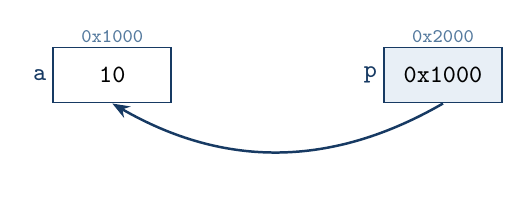
\begin{tikzpicture}
  \cell{a}{0,0}{a}{10}\addr{a}{0x1000}\pcell{p}{4.2,0}{p}{0x1000}\addr{p}{0x2000}
  \draw[ptr] (p.south) to[out=-150,in=-30] (a.south);
\end{tikzpicture}\figcap{题图 1\quad 两行代码执行后的内存}\end{center}
\choices{\cc{p} 的值是 10}{\cc{*p} 的值是 10}{\cc{\&p} 与 \cc{\&a} 相等}{\cc{*p} 的值是 \cc{a} 的地址}

\q{1}{K1 内存与地址}
关于内存地址，下列说法正确的是（\quad{}）
\begin{center}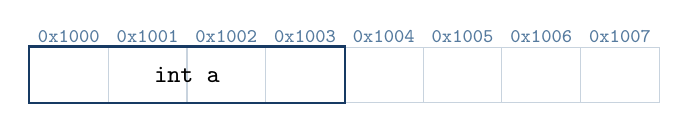
\begin{tikzpicture}
  \foreach \i in {0,...,7} \node[draw=gridc,minimum width=10mm,minimum height=7mm] (c\i) at (\i*1.0,0) {};
  \foreach \i/\h in {0/0,1/1,2/2,3/3,4/4,5/5,6/6,7/7} \node[ad] at (c\i.north) {0x100\h};
  \node[draw=mainc,line width=0.9pt,fit=(c0)(c3),inner sep=0pt,label={[font=\ttfamily\small]center:int a}] {};
\end{tikzpicture}\figcap{题图 2\quad 一个 \texttt{int} 变量在字节编号的内存中}\end{center}
\choices{内存中每个字节都有一个编号，即地址}{地址只能用十六进制表示}{变量名就是变量的地址}{\cc{int} 变量占 4 字节，所以它有 4 个“变量地址”}

\q{1}{K2 指针定义语法}
要定义一个指向 \cc{int} 的指针变量 \cc{p}，下列写法正确的是（\quad{}）
\choices{\cc{int p*;}}{\cc{int *p;}}{\cc{*int p;}}{\cc{int p = \&a;}}

\q{1}{K3 指针的大小}
在 64 位程序中执行 \cc{double d = 3.14; double *pd = \&d;}，则 \cc{sizeof(pd)} 的值为（\quad{}）
\begin{center}\begin{tikzpicture}
  \cell{d}{0,0}{d}{3.14}\pcell{pd}{4.4,0}{pd}{\&d}
  \draw[ptr] (pd.south) to[out=-150,in=-30] (d.south);
  \draw[decorate,decoration={brace,mirror,amplitude=3pt},draw=auxc] (pd.south west) -- (pd.south east) node[midway,below=3pt,note]{? 字节};
\end{tikzpicture}\figcap{题图 4}\end{center}
\choices{4}{8}{16}{与 \cc{d} 的值有关}

\q{1}{K4 空指针}
执行 \cc{int *p = nullptr;} 后，下列说法正确的是（\quad{}）。四个选项所描述的情形分别画在下面：
\par\noindent
\optpanel{A}{\cell{a}{0,0}{a}{?}\pcell{p}{3.8,0}{p}{0}\draw[ptr] ([xshift=-4.5mm]p.west) -- (a.east);\node[note] at (1.9,-0.85){“p 指向某个 int 变量”};}\hfill
\optpanel{B}{\node[draw=gridc,fill=white,minimum width=15mm,minimum height=7mm,font=\ttfamily\small] (z) at (0,0) {100};\node[ad] at (z.north){0x0000};\pcell{p}{3.8,0}{p}{0}\draw[ptr] ([xshift=-4.5mm]p.west) -- (z.east);\node[note] at (1.9,-0.85){“执行 \texttt{*p = 100;}”};}\par\noindent
\optpanel{C}{\pcell{p}{3.8,0}{p}{0}\node[draw=gridc,dashed,minimum width=15mm,minimum height=7mm] (z) at (0,0) {};\draw[ptr,dashed] ([xshift=-4.5mm]p.west) -- (z.east);\node[note] at (1.9,-0.85){“不指向任何对象，不能解引用”};}\hfill
\optpanel{D}{\node[pcell,minimum width=1mm] (p) at (2,0) {};\node[vn] at (p.west){p};\node[note] at (2,-0.85){“p 占用 0 字节”};}
\choices{\cc{p} 指向某个 \cc{int} 变量}{可以执行 \cc{*p = 100;}}{\cc{p} 不指向任何对象，不能解引用}{\cc{p} 占用 0 字节}

\q{1}{K5 野指针}
设 \cc{a} 是已定义的 \cc{int} 变量，\cc{arr} 是已定义的 \cc{int} 数组，下列均为\textbf{函数内的局部定义}。会使 \cc{p} 成为野指针的是（\quad{}）
\par\noindent
\optpanel{A}{\cell{a}{0,0}{a}{5}\pcell{p}{3.8,0}{p}{\&a}\draw[ptr] ([xshift=-4.5mm]p.west) -- (a.east);\node[note] at (1.9,-0.85){\texttt{int *p = \&a;}};}\hfill
\optpanel{B}{\pcell{p}{3.8,0}{p}{nullptr}\node[note] at (1.9,-0.85){\texttt{int *p = nullptr;}};}\par\noindent
\optpanel{C}{\pcell{p}{3.8,0}{p}{?}\node[note] at (1.9,-0.85){\texttt{int *p;}};}\hfill
\optpanel{D}{\arr{r}{-0.6,0}{1,2,3}{arr}\pcell{p}{3.8,0}{p}{arr}\node[note] at (1.9,-0.95){\texttt{int *p = arr;}};}
\choices{\cc{int *p = \&a;}}{\cc{int *p = nullptr;}}{\cc{int *p;}}{\cc{int *p = arr;}}

\q{1}{K6 const 修饰指针}
设 \cc{int a = 10, b = 20; const int *p = \&a;}，下列语句能通过编译的是（\quad{}）
\begin{center}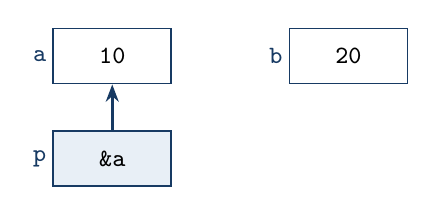
\begin{tikzpicture}
  \cell{a}{0,0}{a}{10}\cell{b}{3,0}{b}{20}\pcell{p}{0,-1.3}{p}{\&a}\draw[ptr] (p.north) -- (a.south);
\end{tikzpicture}\figcap{题图 7\quad 声明后的初始状态}\end{center}
\choices{\cc{*p = 20;}}{\cc{p = \&b;}}{A、B 都可以}{A、B 都不可以}

\q{1}{K6 const 修饰指针}
设 \cc{int a = 10, b = 20; int * const p = \&a;}，下列语句能通过编译的是（\quad{}）
\begin{center}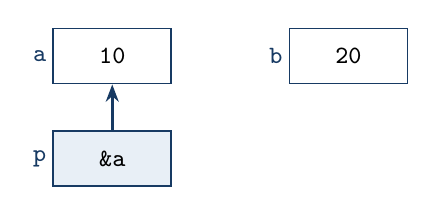
\begin{tikzpicture}
  \cell{a}{0,0}{a}{10}\cell{b}{3,0}{b}{20}\pcell{p}{0,-1.3}{p}{\&a}\draw[ptr] (p.north) -- (a.south);
\end{tikzpicture}\figcap{题图 8\quad 声明后的初始状态}\end{center}
\choices{\cc{p = \&b;}}{\cc{*p = 20;}}{\cc{p++;}}{以上都不能}

\q{1}{K7 指针算术}
执行 \cc{int arr[] = \{1, 2, 3, 4, 5\}; int *p = arr; p++;} 后，\cc{*p} 的值为（\quad{}）
\begin{center}\begin{tikzpicture}
  \arr{A}{0,0}{1,2,3,4,5}{arr}\pcell{p}{0,-1.5}{p}{arr}\draw[ptr] (p.north) -- ([yshift=-3mm]A-0.south);
  \node[note,anchor=west] at (1.2,-1.5) {执行 \texttt{p++} \textbf{之前}};
\end{tikzpicture}\figcap{题图 9}\end{center}
\choices{1}{2}{\cc{arr} 的地址加 1}{5}

\q{1}{K8 值传递}
下列程序的输出是（\quad{}）
\begin{code}
void swap(int a, int b) { int t = a; a = b; b = t; }
int main() {
    int a = 10, b = 20;
    swap(a, b);
    cout << "a=" << a << " b=" << b << endl;
}
\end{code}
\begin{center}\begin{tikzpicture}
  \node[frame,minimum width=38mm,minimum height=17mm] (M) at (0,0) {};
  \node[font=\sffamily\small\bfseries,text=mainc,anchor=north west] at (M.north west) {main};
  \cell{a}{0.3,0.05}{a}{10}\cell{b}{0.3,-0.55}{b}{20}
  \node[frame,minimum width=38mm,minimum height=17mm,fill=warmc] (S) at (5.2,0) {};
  \node[font=\sffamily\small\bfseries,text=beigec,anchor=north west] at (S.north west) {swap(int a, int b)};
  \draw[->,draw=auxc,line width=0.8pt] (M.east) -- node[above,note]{调用} (S.west);
\end{tikzpicture}\figcap{题图 10\quad 调用前 main 中的变量}\end{center}
\choices{\cc{a=20 b=10}}{\cc{a=10 b=20}}{编译错误}{输出不确定}

\needspace{12\baselineskip}\subsubsection*{A-2\quad 多项选择题（5 道）}

\q{1}{K2 \texttt{\&} 与 \texttt{*}}
设 \cc{int a = 5; int *p = \&a;}，下列表达式中值\textbf{等于 5} 的有（\quad{}）
\begin{center}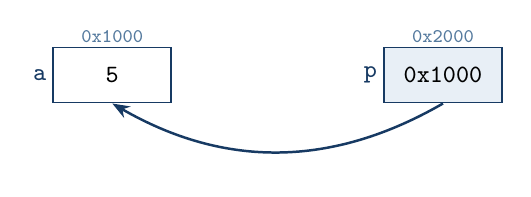
\begin{tikzpicture}
  \cell{a}{0,0}{a}{5}\addr{a}{0x1000}\pcell{p}{4.2,0}{p}{0x1000}\addr{p}{0x2000}
  \draw[ptr] (p.south) to[out=-150,in=-30] (a.south);
\end{tikzpicture}\figcap{题图 11}\end{center}
\choices{\cc{*p}}{\cc{a}}{\cc{*\&a}}{\cc{\&*p}}

\q{1}{K4 K5 空指针与野指针}
关于空指针与野指针，下列说法正确的有（\quad{}）
\begin{center}\begin{tikzpicture}
  \node[draw=badc,fill=redbg,minimum width=26mm,minimum height=8mm,font=\sffamily\scriptsize,align=center] (z) at (0,0) {地址 0 附近};
  \node[draw=gridc,minimum width=26mm,minimum height=8mm,font=\sffamily\scriptsize] (o) at (2.8,0) {不属于本程序};
  \node[draw=mainc,fill=lightc,minimum width=30mm,minimum height=8mm,font=\sffamily\scriptsize] (m) at (5.9,0) {本程序申请的空间};
\end{tikzpicture}\figcap{题图 12\quad 简化的内存地图}\end{center}
\choices{空指针可以用来初始化指针变量}{野指针指向的内存不是程序申请的空间}{对空指针解引用是安全的，只是会得到 0}{定义指针时若暂时无处可指，应初始化为 \cc{nullptr}}

\q{1}{K6 const 修饰指针}
设 \cc{int a = 10, b = 20; const int * const p = \&a;}，下列语句中\textbf{不能}通过编译的有（\quad{}）
\begin{center}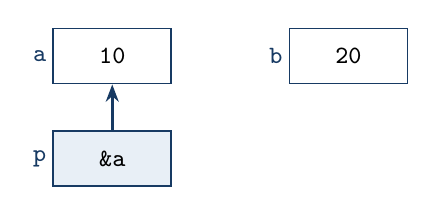
\begin{tikzpicture}
  \cell{a}{0,0}{a}{10}\cell{b}{3,0}{b}{20}\pcell{p}{0,-1.3}{p}{\&a}\draw[ptr] (p.north) -- (a.south);
\end{tikzpicture}\figcap{题图 13}\end{center}
\choices{\cc{p = \&b;}}{\cc{*p = 30;}}{\cc{cout << *p;}}{\cc{int x = *p + 1;}}

\q{1}{K7 数组与指针}
设 \cc{int arr[5] = \{10, 20, 30, 40, 50\}; int *p = arr;}，下列表达式中值\textbf{等于 30} 的有（\quad{}）
\begin{center}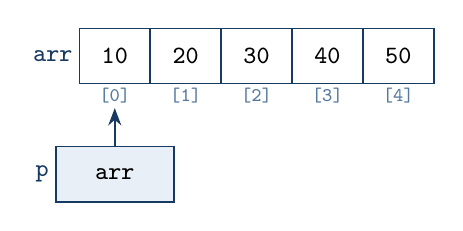
\begin{tikzpicture}
  \arr{A}{0,0}{10,20,30,40,50}{arr}\pcell{p}{0,-1.5}{p}{arr}\draw[ptr] (p.north) -- ([yshift=-3mm]A-0.south);
\end{tikzpicture}\figcap{题图 14}\end{center}
\choices{\cc{*(p + 2)}}{\cc{p[2]}}{\cc{arr[2]}}{\cc{*p + 2}}

\q{1}{K3 K9 sizeof 与数组传参}
设 64 位程序中有 \cc{int arr[6];}，并有函数 \cc{void f(int *a);}。下列说法正确的有（\quad{}）
\begin{center}\begin{tikzpicture}
  \arr{A}{0,0}{,,,,,}{arr}\node[note,anchor=west] at (5.3,0) {main 中定义的数组};
  \node[frame,fill=warmc,minimum width=36mm,minimum height=10mm] (F) at (1.8,-1.6) {};
  \node[font=\ttfamily\small,anchor=west] at (F.west) {\ f(int *a)};
  \draw[->,draw=auxc] ([yshift=-3mm]A-3.south) -- node[right,note]{调用 \texttt{f(arr)}} ([xshift=12mm]F.north);
\end{tikzpicture}\figcap{题图 15}\end{center}
\choices{\cc{sizeof(int*) == sizeof(char*)}}{\cc{sizeof(p)} 的大小由 \cc{p} 所指变量的值决定}{在 main 中 \cc{sizeof(arr)/sizeof(arr[0])} 等于 6}{在 \cc{f} 中 \cc{sizeof(a)/sizeof(a[0])} 仍等于 6}

\needspace{12\baselineskip}\subsubsection*{A-3\quad 填空题（5 道）}

\q{1}{K2 解引用修改变量}
执行 \cc{int a = 10; int *p = \&a; *p = 100;} 后，\cc{a} = \blank[1.5cm]，\cc{*p} = \blank[1.5cm]。
\begin{center}\begin{tikzpicture}
  \cell{a}{0,0}{a}{10}\pcell{p}{4.2,0}{p}{\&a}\draw[ptr] (p.south) to[out=-150,in=-30] (a.south);
  \node[note,anchor=west] at (5.2,0) {执行第三句 \textbf{之前}};
\end{tikzpicture}\figcap{题图 16}\end{center}

\q{1}{K3 指针的大小}
在 64 位程序中 \cc{sizeof(int*)} = \blank[1.5cm] 字节；在 32 位程序中 \cc{sizeof(int*)} = \blank[1.5cm] 字节。
\begin{center}\begin{tikzpicture}
  \node[pcell,minimum width=40mm] (p64) at (0,0) {64 位地址}; \node[vn] at (p64.west) {64 位程序};
  \node[pcell,minimum width=20mm] (p32) at (7,0) {32 位地址}; \node[vn] at (p32.west) {32 位程序};
\end{tikzpicture}\figcap{题图 17\quad 指针中保存的地址宽度}\end{center}

\q{1}{K9 sizeof 求数组长度}
设 \cc{int arr[] = \{3, 7, 9, 12, 5, 1\};}，则\\ \cc{sizeof(arr)} = \blank[1.5cm]，\cc{sizeof(arr)/sizeof(arr[0])} = \blank[1.5cm]。
\begin{center}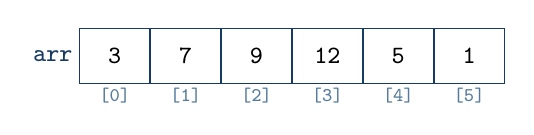
\begin{tikzpicture}
  \arr{A}{0,0}{3,7,9,12,5,1}{arr}
\end{tikzpicture}\figcap{题图 18}\end{center}

\q{1}{K1 K7 地址计算}
设 \cc{int arr[5];} 的首地址为 \cc{0x1000}，\cc{int *p = arr;}，则 \cc{p + 3} 的值为 \blank{}，\cc{*(p + 3)} 就是 \cc{arr[}\blank[1cm]\cc{]}。
\begin{center}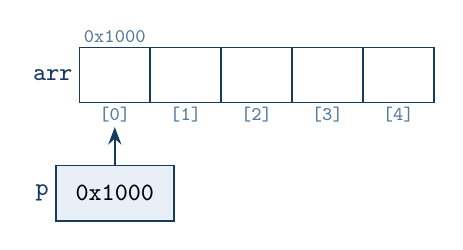
\begin{tikzpicture}
  \arr{A}{0,0}{,,,,}{arr}\node[ad] at (A-0.north) {0x1000};
  \pcell{p}{0,-1.5}{p}{0x1000}\draw[ptr] (p.north) -- ([yshift=-3mm]A-0.south);
\end{tikzpicture}\figcap{题图 19\quad 只标出了首元素地址}\end{center}

\q{1}{K10 冒泡排序循环}
对 5 个元素做冒泡排序（外层 \cc{i} 从 0 开始），外层最多 \blank[1.2cm] 轮；当 \cc{i = 1} 时内层比较 \blank[1.2cm] 次；全部比较次数为 \blank[1.2cm] 次。
\begin{center}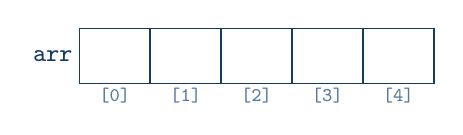
\begin{tikzpicture}
  \arr{A}{0,0}{,,,,}{arr}
\end{tikzpicture}\figcap{题图 20\quad 5 个元素}\end{center}

\needspace{12\baselineskip}\subsubsection*{A-4\quad 解答题（5 道）}

\q{1}{K2 定义、赋值与解引用}
阅读程序，(1) 画出每条语句执行后的内存图；(2) 写出输出结果。
\begin{code}
int a = 10, b = 20;
int *p = &a;
*p = 30;
p = &b;
*p = 40;
cout << a << " " << b << " " << *p << endl;
\end{code}
\begin{center}\begin{tikzpicture}
  \cell{a}{0,0}{a}{10}\addr{a}{0x1000}\cell{b}{3.4,0}{b}{20}\addr{b}{0x1004}\pcell{p}{0,-1.4}{p}{?}
  \node[note,anchor=west] at (1.2,-1.4) {第 1 行执行后；\texttt{p} 尚未定义};
\end{tikzpicture}\figcap{题图 21\quad 起始状态}\end{center}

\q{1}{K6 const 三种情况}
设 \cc{int a = 1, b = 2;} 且
\begin{code}
const int *p1 = &a;
int * const p2 = &a;
const int * const p3 = &a;
\end{code}
判断下列语句能否通过编译，并说明理由：\ci{①} \cc{*p1 = 5;}\quad \ci{②} \cc{p1 = \&b;}\quad \ci{③} \cc{*p2 = 5;}\quad \ci{④} \cc{p2 = \&b;}\quad \ci{⑤} \cc{*p3 = 5;}\quad \ci{⑥} \cc{a = 5;}
\begin{center}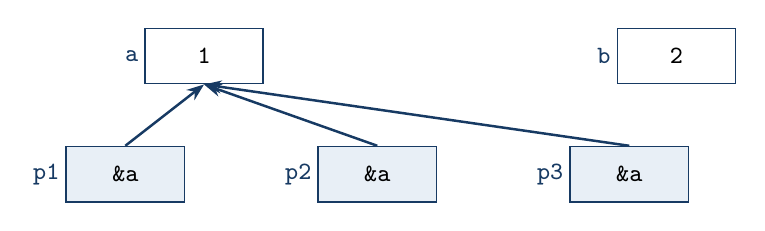
\begin{tikzpicture}
  \cell{a}{0,0}{a}{1}\cell{b}{6,0}{b}{2}
  \pcell{p1}{-1,-1.5}{p1}{\&a}\pcell{p2}{2.2,-1.5}{p2}{\&a}\pcell{p3}{5.4,-1.5}{p3}{\&a}
  \foreach \q in {p1,p2,p3} \draw[ptr] (\q.north) -- (a.south);
\end{tikzpicture}\figcap{题图 22\quad 三个指针都指向 a}\end{center}

\q{1}{K8 值传递与地址传递}
(1) 写出上面第 10 题程序的输出，并画图说明 \cc{swap} 为什么没有交换 \cc{main} 中的 \cc{a}、\cc{b}；(2) 把 \cc{swap} 改写成地址传递版本 \cc{swap\_p}，写出调用语句，并说明它为什么能交换。

\q{1}{K5 K7 指针遍历与越界}
阅读程序，回答：(1) 输出是什么？(2) 循环结束后 \cc{p} 指向哪里？此时能否执行 \cc{cout << *p;}？(3) 笔记原代码数组有 5 个元素却写 \cc{i < 10}，有什么问题？应怎样修改？
\begin{code}
int arr[] = {2, 4, 6, 8};
int *p = arr;
for (int i = 0; i < 4; i++) { cout << *p << " "; p++; }
\end{code}
\begin{center}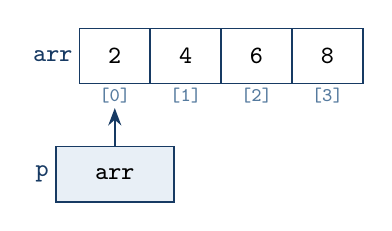
\begin{tikzpicture}
  \arr{A}{0,0}{2,4,6,8}{arr}\pcell{p}{0,-1.5}{p}{arr}\draw[ptr] (p.north) -- ([yshift=-3mm]A-0.south);
\end{tikzpicture}\figcap{题图 24\quad 循环开始前}\end{center}

\q{1}{K10 冒泡排序过程}
对数组 \cc{\{6, 2, 8, 4, 1\}} 进行升序冒泡排序。(1) 写出第 1 轮（\cc{i = 0}）中每一次比较后的数组状态；(2) 写出第 2 轮结束后的数组。
\begin{center}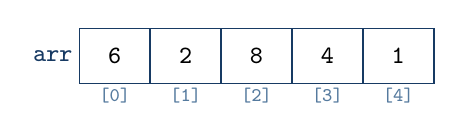
\begin{tikzpicture}
  \arr{A}{0,0}{6,2,8,4,1}{arr}
\end{tikzpicture}\figcap{题图 25}\end{center}

% ----------------------------------------------------------------
\needspace{12\baselineskip}\usubsection{B. 中等偏下提升训练（10 道）}
\needspace{12\baselineskip}\subsubsection*{B-1\quad 单项选择题（3 道）}

\q{2}{K7 K2 指针偏移}
设 \cc{int arr[] = \{1, 2, 3, 4, 5\}; int *p = arr + 1;}，则 \cc{*(p + 2)} 的值为（\quad{}）
\begin{center}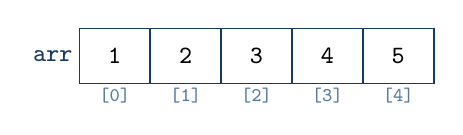
\begin{tikzpicture}
  \arr{A}{0,0}{1,2,3,4,5}{arr}
\end{tikzpicture}\figcap{题图 26}\end{center}
\choices{3}{4}{5}{2}

\q{2}{K8 K2 指针形参也是拷贝}
下列程序执行后，\cc{a} 的值和 \cc{p} 的状态是（\quad{}）
\begin{code}
void f(int *q) {
    *q = *q * 2;
    q = nullptr;
}
int main() {
    int a = 5;
    int *p = &a;
    f(p);
}
\end{code}
\begin{center}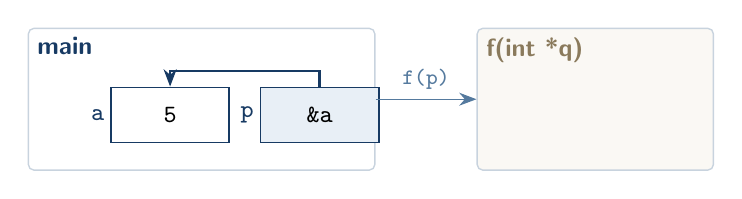
\begin{tikzpicture}
  \node[frame,minimum width=44mm,minimum height=18mm] (M) at (0,0) {};
  \node[font=\sffamily\small\bfseries,text=mainc,anchor=north west] at (M.north west) {main};
  \cell{a}{-0.4,-0.2}{a}{5}\pcell{p}{1.5,-0.2}{p}{\&a}
  \draw[ptr] (p.north) |- ([yshift=2mm]a.north) -- (a.north);
  \node[frame,minimum width=30mm,minimum height=18mm,fill=warmc] (S) at (5,0) {};
  \node[font=\sffamily\small\bfseries,text=beigec,anchor=north west] at (S.north west) {f(int *q)};
  \draw[->,draw=auxc] (M.east) -- node[above,note]{\texttt{f(p)}} (S.west);
\end{tikzpicture}\figcap{题图 27\quad 调用前}\end{center}
\choices{\cc{a = 10}，\cc{p} 变为空指针}{\cc{a = 10}，\cc{p} 仍指向 \cc{a}}{\cc{a = 5}，\cc{p} 变为空指针}{\cc{a = 5}，\cc{p} 仍指向 \cc{a}}

\q{2}{K6 K7 常量指针在数组上}
设 \cc{int arr[] = \{1, 2, 3\}; const int *p = arr;}，下列代码能通过编译的是（\quad{}）
\begin{center}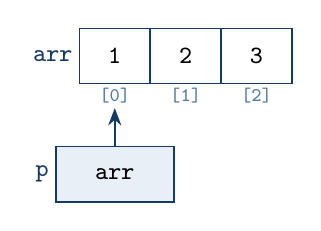
\begin{tikzpicture}
  \arr{A}{0,0}{1,2,3}{arr}\pcell{p}{0,-1.5}{p}{arr}\draw[ptr] (p.north) -- ([yshift=-3mm]A-0.south);
\end{tikzpicture}\figcap{题图 28}\end{center}
\choices{\cc{p++; cout << *p;}}{\cc{*p = 0;}}{\cc{p[1] = 5;}}{\cc{*(p + 1) = 5;}}

\needspace{12\baselineskip}\subsubsection*{B-2\quad 多项选择题（2 道）}

\q{2}{K3 K9 数组传参后的 sizeof}
64 位程序如下，下列说法正确的有（\quad{}）
\begin{code}
void show(int *a) { cout << sizeof(a) << endl; }
int main() {
    int arr[10];
    cout << sizeof(arr) << endl;
    show(arr);
}
\end{code}
\choices{main 中输出 40}{\cc{show} 中输出 8}{在 \cc{show} 中 \cc{sizeof(a)/sizeof(a[0])} 等于 10}{因此排序函数通常需要额外传入长度 \cc{n}}

\q{2}{K10 K5 冒泡排序边界}
笔记封装版冒泡排序的内层循环误写为 \cc{for (int j = 0; j < n - j - 1; j++)}。对数组 \cc{\{3, 7, 9, 12, 5, 1\}}（$n=6$）调用该函数，下列说法正确的有（\quad{}）
\begin{center}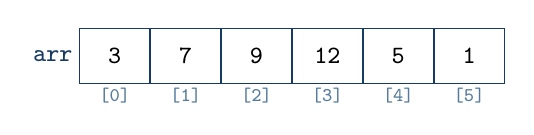
\begin{tikzpicture}
  \arr{A}{0,0}{3,7,9,12,5,1}{arr}
\end{tikzpicture}\figcap{题图 30}\end{center}
\choices{输出仍为 \cc{3 7 9 12 5 1}}{每一轮中 \cc{j} 只能取 0、1、2}{改为 \cc{j < n - i - 1} 后输出 \cc{1 3 5 7 9 12}}{该错误会导致 \cc{arr[j+1]} 越界访问}

\needspace{12\baselineskip}\subsubsection*{B-3\quad 填空题（3 道）}

\q{2}{K7 指针与数组综合}
执行下列代码后，数组 \cc{arr} 为 \cc{\{}\blank[0.9cm]\cc{,}\blank[0.9cm]\cc{,}\blank[0.9cm]\cc{,}\blank[0.9cm]\cc{\}}，此时 \cc{p} 指向 \cc{arr[}\blank[0.8cm]\cc{]}。
\begin{code}
int arr[] = {10, 20, 30, 40};
int *p = arr;
*(p + 1) += 5;
p += 2;
*p = *(p - 1) + 1;
\end{code}
\begin{center}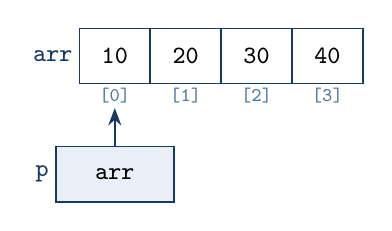
\begin{tikzpicture}
  \arr{A}{0,0}{10,20,30,40}{arr}\pcell{p}{0,-1.5}{p}{arr}\draw[ptr] (p.north) -- ([yshift=-3mm]A-0.south);
\end{tikzpicture}\figcap{题图 31\quad 第 2 行执行后}\end{center}

\q{2}{K10 比较与交换次数}
对 6 个元素做冒泡排序（按笔记的两层循环，不提前结束）：总比较次数为 \blank[1.2cm]；若原数组已经升序，交换次数为 \blank[1.2cm]；若原数组为 \cc{\{6,5,4,3,2,1\}}，交换次数为 \blank[1.2cm]。
\begin{center}\begin{tikzpicture}
  \arr{A}{0,0}{6,5,4,3,2,1}{逆序}\arr{B}{7,0}{1,2,3,4,5,6}{升序}
\end{tikzpicture}\figcap{题图 32}\end{center}

\q{2}{K1 K3 K7 地址与步长}
64 位程序中，\cc{double arr[4];} 的首地址为 \cc{0x2000}，\cc{double *q = \&arr[3];}。则 \cc{q} 的值为 \blank{}，\cc{q - arr} = \blank[1.2cm]，\cc{sizeof(q)} = \blank[1.2cm]。\\
{\small{}（提示：指向同一数组的两个指针相减，结果是它们之间相隔的\textbf{元素个数}。）}
\begin{center}\begin{tikzpicture}
  \arr{A}{0,0}{,,,}{arr}\node[ad] at (A-0.north) {0x2000};
  \node[note,anchor=west] at (3.4,0) {每个元素是 \texttt{double}};
\end{tikzpicture}\figcap{题图 33}\end{center}

\needspace{12\baselineskip}\subsubsection*{B-4\quad 综合大题（2 道）}

\q{2}{K6 K8 K9 用指针“返回”两个结果}
一个函数只能 \cc{return} 一个值。现在希望一次求出数组的最小值和最大值，设计函数
\begin{code}
void minmax(const int *arr, int n, int *pmin, int *pmax);
\end{code}
(1) 为什么 \cc{pmin}、\cc{pmax} 要设计成指针？为什么 \cc{arr} 前面加 \cc{const}？\\
(2) 补全函数体。\\
(3) 在 \cc{main} 中执行 \cc{int a[] = \{4, 9, 1, 7\}; int mn, mx; minmax(a, 4, \&mn, \&mx);}，画出函数即将返回时的内存图，并写出 \cc{mn}、\cc{mx} 的值。
\begin{center}\begin{tikzpicture}
  \node[frame,minimum width=64mm,minimum height=22mm] (M) at (1.6,-0.35) {};
  \node[font=\sffamily\small\bfseries,text=mainc,anchor=north west] at (M.north west) {main};
  \arr{A}{0,0}{4,9,1,7}{a}\cell{mn}{0.2,-1.15}{mn}{?}\cell{mx}{3,-1.15}{mx}{?}
  \node[frame,fill=warmc,minimum width=48mm,minimum height=22mm] (F) at (8.4,-0.35) {};
  \node[font=\sffamily\small\bfseries,text=beigec,anchor=north west] at (F.north west) {minmax(arr, n, pmin, pmax)};
\end{tikzpicture}\figcap{题图 34\quad 调用前}\end{center}

\q{2}{K9 K10 排序函数的调试与改进}
笔记中封装的冒泡排序如下（第 392 页原样）：
\begin{code}
void BubbleSort(int *arr, int n)
{
    for (int i = 0; i < n - 1; i++)
        for (int j = 0; j < n - j - 1; j++)
            if arr[j] > arr[j+1]
            { int temp = arr[j]; arr[j] = arr[j+1]; arr[j+1] = temp; }
}
\end{code}
(1) 指出其中的两处错误并改正；\\
(2) 用改正后的函数对 \cc{\{3, 7, 9, 12, 5, 1\}} 排序，写出每一轮结束后的数组；\\
(3) 若数组本来就是 \cc{\{1, 2, 3, 4, 5, 6\}}，改正后的函数共比较几次？如果增加一个标志变量 \cc{swapped}，在某一轮没有发生任何交换时立即结束，则需要比较几次？
\begin{center}\begin{tikzpicture}
  \arr{A}{0,0}{3,7,9,12,5,1}{arr}
\end{tikzpicture}\figcap{题图 35}\end{center}

% ----------------------------------------------------------------
\needspace{12\baselineskip}\usubsection{C. 跨学科迁移训练（3 道）}
\noindent{\small\color{violetc}本组题目的背景来自其他课程，但\textbf{完成本题所需的背景信息都已在题干中给出}，真正考查的仍是本章知识。}

\q{3}{K2 × 数据结构}
\textbf{背景（数据结构 · 链表）}：链表把数据分散存放在若干“结点”中，每个结点除了保存数据 \cc{val}，还保存下一个结点的地址 \cc{next}；最后一个结点的 \cc{next} 为 \cc{nullptr}。代码中 \cc{p->val} 等价于 \cc{(*p).val}，意思是“先解引用 \cc{p} 找到结点，再取它的 \cc{val}”。
\begin{code}
struct Node { int val; Node *next; };
Node n3 = {3, nullptr};
Node n2 = {2, &n3};
Node n1 = {1, &n2};
Node *p = &n1;
p = p->next;
cout << p->val << endl;
\end{code}
\begin{center}\begin{tikzpicture}
  \foreach \n/\x/\v/\nx in {n1/0/1/\&n2,n2/3.6/2/\&n3,n3/7.2/3/nullptr} {
    \node[acell,minimum width=10mm] (\n v) at (\x,0) {\v};
    \node[acell,fill=formc,minimum width=16mm,anchor=west] (\n n) at (\n v.east) {\nx};
    \node[ad] at (\n v.north) {val}; \node[ad] at (\n n.north) {next};
    \node[vn,anchor=north] at ([yshift=-1mm]\n v.south) {\n};}
  \draw[ptr] (n1n.east) -- (n2v.west); \draw[ptr] (n2n.east) -- (n3v.west);
  \pcell{p}{0,-1.8}{p}{\&n1}\draw[ptr] (p.north) -- ([yshift=-5mm]n1v.south);
\end{tikzpicture}\figcap{题图 36\quad 三个结点组成的链表（执行 \texttt{p = p->next} 之前）}\end{center}
输出为（\quad{}）
\choices{1}{2}{3}{编译错误}

\q{3}{K2 K5 × 嵌入式系统}
\textbf{背景（嵌入式 · 寄存器）}：某单片机的芯片手册规定，地址 \cc{0x40020014} 处是控制 LED 引脚的“输出寄存器”，向它写入 1 可以点亮 LED。程序如下（\cc{volatile} 的作用是告诉编译器每次都真实地读写这个地址，本题可以忽略它）：
\begin{code}
volatile unsigned int *reg = (volatile unsigned int *)0x40020014;
*reg = 1;      // 点亮 LED
\end{code}
\begin{center}\begin{tikzpicture}
  \node[draw=mainc,fill=lightc,minimum width=48mm,minimum height=8mm,font=\sffamily\small] (r) at (0,0) {LED 输出寄存器};
  \node[ad] at (r.north) {0x40020014（芯片手册规定）};
  \pcell{p}{5.8,0}{reg}{0x40020014}
  \draw[ptr] (p.south) to[out=-150,in=-30] (r.south);
\end{tikzpicture}\figcap{题图 37}\end{center}
下列说法正确的有（\quad{}）
\choices{这里把整数地址强制转换为指针，与笔记中 \cc{(int*)0x0010} 的写法形式相同}{在普通电脑程序中，随便写一个地址这样访问同样是安全的}{能否访问，取决于这个地址是否是程序可以合法访问的空间（这里由芯片手册保证）}{\cc{*reg = 1} 是通过解引用向该地址写入数据}

\q{3}{K1 K7 × 图像处理}
\textbf{背景（图像处理 · 像素数组）}：一张宽 $W=4$、高 $H=3$ 的灰度图片，每个像素用 1 个字节（\cc{unsigned char}）表示亮度，所有像素\textbf{按行依次}存放在一个一维数组中，第 $r$ 行第 $c$ 列（$r,c$ 都从 0 开始）的像素下标为 $r\times W+c$。
\begin{center}\begin{tikzpicture}
  \foreach \r in {0,1,2} \foreach \c in {0,...,3} {
    \node[draw=gridc,minimum size=7mm,font=\ttfamily\tiny,text=auxc] at (\c*0.75,-\r*0.75) {(\r,\c)};}
  \node[note] at (1.1,0.65) {图片（3 行 4 列）};
  \draw[->,draw=auxc,line width=0.8pt] (3.0,-0.75) -- (4.2,-0.75) node[midway,below=2pt,note]{按行\\展开};
  \foreach \k in {0,...,11} \node[draw=mainc,minimum width=6mm,minimum height=7mm,font=\ttfamily\tiny] (e\k) at (4.6+\k*0.6,-0.75) {\k};
  \node[ad] at (e0.north) {0x3000};
  \node[note] at (8,-1.5) {一维数组（框内数字为下标）};
\end{tikzpicture}\figcap{题图 38}\end{center}
设 \cc{unsigned char *img} 指向下标 0 的像素，地址为 \cc{0x3000}。第 2 行第 1 列的像素下标为 \blank[1.2cm]，地址为 \blank{}，可以写成 \cc{*(img +}\blank[1.2cm]\cc{)}。若改为每个像素用 4 字节的 \cc{int} 存放，\cc{int *q} 指向 \cc{0x3000}，则同一个像素的地址为 \blank{}。

% ================================================================
%  答案速查 + 详细解析（A 组、B 组、C 组）
%  所有答案均经 g++ 实际编译 / 运行核对
% ================================================================
\clearpage
\usection{全部答案速查}
\noindent{\small 只列结果，过程见后面的详细解析。所有涉及代码的答案均已用 g++（C++17，64 位 Linux）编译或运行核对。}

\begin{center}
\renewcommand{\arraystretch}{1.3}
\noindent\begin{tabularx}{\linewidth}{@{}p{2.6cm}Y@{}}
\toprule
\rowcolor{lightc}\multicolumn{2}{@{}l}{\sffamily\bfseries\color{mainc} A 组 基础巩固} \\
单选 1--10 & 1.\,B\quad 2.\,A\quad 3.\,B\quad 4.\,B\quad 5.\,C\quad 6.\,C\quad 7.\,B\quad 8.\,B\quad 9.\,B\quad 10.\,B \\
多选 11--15 & 11.\,ABC\quad 12.\,ABD\quad 13.\,AB\quad 14.\,ABC\quad 15.\,AC \\
填空 16--20 & 16.\ 100，100\quad 17.\ 8，4\quad 18.\ 24，6\quad 19.\ \cc{0x100C}，3\quad 20.\ 4，3，10 \\
解答 21--25 & 21.\ 输出 \cc{30 40 40}\quad 22.\ \ci{①}\xmark\ \ci{②}\cmark\ \ci{③}\cmark\ \ci{④}\xmark\ \ci{⑤}\xmark\ \ci{⑥}\cmark\quad 23.\ 输出 \cc{a=10 b=20}；改为 \cc{swap\_p(\&a,\&b)}\quad 24.\ \cc{2 4 6 8}；\cc{p} 指向 \cc{arr+4}，不能解引用；改为 \cc{i < len}\quad 25.\ 第 1 轮末 \cc{2 6 4 1 8}；第 2 轮末 \cc{2 4 1 6 8} \\
\midrule
\rowcolor{lightc}\multicolumn{2}{@{}l}{\sffamily\bfseries\color{mainc} B 组 中等偏下提升} \\
单选 26--28 & 26.\,B\quad 27.\,B\quad 28.\,A \\
多选 29--30 & 29.\,ABD\quad 30.\,ABC \\
填空 31--33 & 31.\ \cc{\{10,25,26,40\}}，2\quad 32.\ 15，0，15\quad 33.\ \cc{0x2018}，3，8 \\
综合 34--35 & 34.\ \cc{mn = 1}，\cc{mx = 9}\quad 35.\ 改 \cc{n-j-1}$\to$\cc{n-i-1}、补 \cc{if} 括号；各轮后依次为 [\cc{3 7 9 5 1 12}] [\cc{3 7 5 1 9 12}] [\cc{3 5 1 7 9 12}] [\cc{3 1 5 7 9 12}] [\cc{1 3 5 7 9 12}]；比较 15 次，加标志后 5 次 \\
\midrule
\rowcolor{lightc}\multicolumn{2}{@{}l}{\sffamily\bfseries\color{mainc} C 组 跨学科迁移} \\
36--38 & 36.\,B\quad 37.\,ACD\quad 38.\ 9，\cc{0x3009}，9，\cc{0x3024} \\
\bottomrule
\end{tabularx}
\end{center}

% ================================================================
\usection{A 组详细解析}
% ================================================================
\needspace{12\baselineskip}\subsection*{A-1\quad 单项选择题}

% ---------- 1 ----------
\sol{1}{B}{1}{K2 取地址与解引用（第二讲）}
\step{对应知识} \cc{p = \&a} 时 \cc{*p} $\equiv$ \cc{a}；\cc{p} 的值是地址。
\step{思路} 先分清图上的四个量：\cc{a}（框内 10）、\cc{\&a}（0x1000）、\cc{p}（框内 0x1000）、\cc{\&p}（0x2000），再逐项对照。
\par\noindent
\optsol{A}{0}{\cell{a}{0,0}{a}{10}\pcell[badcell]{p}{3.8,0}{p}{10}\node[bnote] at (1.9,-0.9){p 框里应是地址 0x1000，不是 10};}{\cc{p} 是指针，保存的是 \cc{a} 的\textbf{地址}，不是 \cc{a} 的值。}\hfill
\optsol{B}{1}{\cell[hl]{a}{0,0}{a}{10}\pcell{p}{3.8,0}{p}{0x1000}\draw[ptrok] ([xshift=-4.5mm]p.west) -- node[above,gnote]{*p} (a.east);}{沿箭头解引用到达 \cc{a}，\cc{*p} 就是 \cc{a}，值为 10。}
\par\noindent
\optsol{C}{0}{\cell{a}{0,0}{a}{10}\addr{a}{0x1000}\pcell{p}{3.8,0}{p}{0x1000}\node[ad,text=badc] at (p.north){0x2000};\node[bnote] at (1.9,-0.8){两个方框上方的地址不同};}{\cc{\&p} 是 \cc{p} 自己的地址（0x2000），\cc{\&a} 是 0x1000，二者是两个不同变量的地址。}\hfill
\optsol{D}{0}{\cell{a}{0,0}{a}{10}\pcell{p}{3.8,0}{p}{0x1000}\node[bnote] at (1.9,-0.8){“a 的地址”是 p 的值，\\不是 *p 的值};}{把 \cc{p} 与 \cc{*p} 混淆了：\cc{a} 的地址是 \cc{p} 的值。}
\step{常见错误} 把“箭头起点”（\cc{p}）和“箭头终点”（\cc{*p}）搞反。
\oneline{\cc{p} 是门牌号，\cc{*p} 是那户人家。}

% ---------- 2 ----------
\sol{2}{A}{1}{K1 内存与地址（第一讲）}
\begin{center}\begin{tikzpicture}
  \foreach \i in {0,...,7} \node[draw=gridc,minimum width=10mm,minimum height=7mm] (c\i) at (\i*1.0,0) {};
  \foreach \i in {0,...,7} \node[ad] at (c\i.north) {0x100\i};
  \node[draw=mainc,line width=0.9pt,fill=hlc,fit=(c0)(c3),inner sep=0pt,label={[font=\ttfamily\small]center:int a}] {};
  \draw[->,draw=okc,line width=0.8pt] (-0.9,0.9) node[left,gnote]{\&a = 0x1000} -- ([yshift=3.5mm]c0.north west);
  \foreach \i in {0,...,7} \draw[okc] ([yshift=-1mm]c\i.south) -- ++(0,-0.25);
  \node[gnote] at (3.5,-0.95) {每个字节都有编号（A 正确）；a 占 4 个字节，但“a 的地址”只有一个（D 错误）};
\end{tikzpicture}\figcap{解析图 2}\end{center}
\step{逐项} (A) 正确，这正是地址的定义。(B) 错误：十六进制只是书写习惯，地址本质是整数，也可以用十进制表示。(C) 错误：变量名是源代码中的标签，地址要用 \cc{\&a} 获得。(D) 错误：变量占 4 个字节（有 4 个字节编号），但\textbf{变量的地址}规定为首字节编号，只有一个（见解析图 2 绿色箭头）。
\oneline{每个字节一个编号，每个变量一个地址（首字节）。}

% ---------- 3 ----------
\sol{3}{B}{1}{K2 指针定义语法（第二讲）}
\step{可视化判定} 本题考查纯语法记忆，画图不能降低难度，故不配图。
\step{判断} 语法为“数据类型 * 指针变量名”，只有 (B) \cc{int *p;} 符合。(A) \cc{*} 位置错误；(C) \cc{*int} 不是合法类型写法；(D) \cc{int p} 是普通整数，不能保存地址（\cc{\&a} 的类型是 \cc{int*}，编译报错）。
\step{常见错误} 写 \cc{int* p, q;} 以为定义了两个指针（见第二讲易错点）。
\oneline{\cc{*} 紧贴变量名：\cc{int *p}。}

% ---------- 4 ----------
\sol{4}{B}{1}{K3 指针的大小（第三讲）}
\begin{center}\begin{tikzpicture}
  \cell{d}{0,0}{d}{3.14}\pcell{pd}{4.4,0}{pd}{\&d}
  \draw[ptr] (pd.south) to[out=-150,in=-30] (d.south);
  \draw[decorate,decoration={brace,amplitude=3pt},draw=okc] (pd.north west) -- (pd.north east) node[midway,above=3pt,gnote]{8 字节：一个 64 位地址};
  \draw[decorate,decoration={brace,amplitude=3pt},draw=auxc] (d.north west) -- (d.north east) node[midway,above=3pt,note]{\texttt{double}：8 字节};
  \node[note,anchor=west] at (5.7,0) {两个 8 只是巧合：\\换成 \texttt{char *pc} 也是 8};
\end{tikzpicture}\figcap{解析图 4}\end{center}
\step{判断} 64 位程序中任何数据指针都是 8 字节（第三讲推导：$64\div8=8$），选 (B)。(A) 是 32 位程序的结果；(C) 无依据；(D) 指针大小与所指对象的值、甚至类型都无关。
\step{常见错误} 看到 \cc{double} 是 8 字节，就以为“\cc{double*} 是 8 字节是因为 \cc{double} 是 8 字节”。
\oneline{指针多大只看地址多宽。}

% ---------- 5 ----------
\sol{5}{C}{1}{K4 空指针（第四讲）}
\par\noindent
\optsol{A}{0}{\cell[badcell]{a}{0,0}{a}{?}\pcell{p}{3.8,0}{p}{0}\draw[ptrbad] ([xshift=-4.5mm]p.west) -- (a.east);\node[bnote] at (1.9,-1.0){这条箭头并不存在};}{空指针的定义就是“不指向任何对象”。}\hfill
\optsol{B}{0}{\node[draw=badc,fill=redbg,minimum width=15mm,minimum height=7mm,font=\ttfamily\small] (z) at (0,0) {100};\node[ad] at (z.north){0x0000};\pic at (z.center) {forbid};\pcell{p}{3.8,0}{p}{0}\draw[ptrbad] ([xshift=-4.5mm]p.west) -- (z.east);}{解引用空指针是未定义行为，常见系统上会段错误。}
\par\noindent
\optsol{C}{1}{\pcell{p}{3.8,0}{p}{0}\node[draw=gridc,dashed,minimum width=15mm,minimum height=7mm] (z) at (0,0) {};\node[gnote] at (0,-0.7){没有目标};}{正是空指针的定义与注意事项（笔记 §7.4）。}\hfill
\optsol{D}{0}{\node[pcell,minimum width=40mm] (p) at (2.2,0) {0};\node[vn] at (p.west){p};\draw[decorate,decoration={brace,mirror,amplitude=3pt},draw=badc] (p.south west) -- (p.south east) node[midway,below=3pt,bnote]{仍占 8 字节};}{\cc{p} 的\textbf{值}为空，但 \cc{p} 这个变量本身照样占 8 字节。}
\step{常见错误} 把“值为空”误解为“不占空间”；或以为 \cc{*p} 会读出 0。
\oneline{空指针：有变量、有值（空），没有目标。}

% ---------- 6 ----------
\sol{6}{C}{1}{K5 野指针（第四讲）}
\par\noindent
\optsol{A}{0}{\cell{a}{0,0}{a}{5}\pcell{p}{3.8,0}{p}{\&a}\draw[ptrok] ([xshift=-4.5mm]p.west) -- (a.east);}{指向已定义的变量，合法。}\hfill
\optsol{B}{0}{\pcell{p}{3.8,0}{p}{nullptr}\node[gnote] at (1.4,0){明确“无指向”};}{空指针不是野指针：它的值是确定的、可检查的。}
\par\noindent
\optsol{C}{1}{\pcell[badcell]{p}{3.8,0}{p}{?}\node[draw=gridc,dashed,minimum width=12mm,minimum height=7mm] (u) at (0,0) {???};\draw[ptrbad] ([xshift=-4.5mm]p.west) -- (u.east);\node[bnote] at (1.8,0.35){随机地址};}{局部指针未初始化，值不确定，指向未知位置——典型野指针。}\hfill
\optsol{D}{0}{\arr{r}{-0.6,0}{1,2,3}{arr}\pcell{p}{3.8,0}{p}{arr}\draw[ptrok] (p.south) to[out=-150,in=-60] ([yshift=-3mm]r-0.south);}{数组名转换为首元素地址，指向合法数组元素。}
\step{补充} 笔记中的另一个来源 \cc{int *p = (int*)0x0010;} 也是野指针，此外还有越界。
\oneline{“定义了却没给值”的指针就是野的。}

% ---------- 7 ----------
\sol{7}{B}{1}{K6 const 修饰指针（第五讲）}
\par\noindent
\optsol{A}{0}{\cell{a}{0,0}{a}{10}\pic at ([xshift=-1mm,yshift=-1mm]a.north east){lock};\pcell{p}{3.8,0}{p}{\&a}\draw[ptr] ([xshift=-4.5mm]p.west) -- (a.east);\node[bnote] at (1.9,-1.0){const 在 * 左：值被锁};}{\cc{*p} 的类型是 \cc{const int}，不能赋值。}\hfill
\optsol{B}{1}{\cell{a}{0,0}{a}{10}\cell{b}{1.9,0}{b}{20}\pcell{p}{4.1,-0.2}{p}{\&b}\draw[ptrok] (p.west) -- (b.east);\node[gnote] at (2.8,-0.9){\texttt{p} 本身没被锁，可改指向};}{\cc{p} 的类型是 \cc{const int*}，最外层无 const，可以改指向。}
\step{C、D} 由上，只有 B 合法，所以 C、D 都错。
\step{三步法} 找 \cc{*} $\to$ const 在左 $\to$ 锁值；A 改的是值（\xmark{}），B 改的是指向（\cmark{}）。
\oneline{const 在 * 左边：锁值不锁指向。}

% ---------- 8 ----------
\sol{8}{B}{1}{K6 const 修饰指针（第五讲）}
\par\noindent
\optsol{A}{0}{\cell{a}{0,0}{a}{10}\cell{b}{1.9,0}{b}{20}\pcell{p}{4.1,-0.2}{p}{\&a}\pic at ([xshift=-1mm,yshift=1mm]p.south east){lock};\draw[ptrbad] (p.west) -- (b.east);}{const 在 * 右边，\cc{p} 本身是常量，不能改指向。}\hfill
\optsol{B}{1}{\cell[hl]{a}{0,0}{a}{20}\pcell{p}{3.8,0}{p}{\&a}\draw[ptrok] ([xshift=-4.5mm]p.west) -- (a.east);\node[gnote] at (1.9,-1.0){a 被改为 20};}{\cc{*p} 类型为普通 \cc{int}，可以赋值。}
\par\noindent
\optsol{C}{0}{\arr{r}{-0.6,0}{a,?}{}\pcell{p}{3.8,0}{p}{\&a}\pic at ([xshift=-1mm,yshift=1mm]p.south east){lock};\draw[ptrbad] (p.south) to[out=-150,in=-60] ([yshift=-3mm]r-1.south);}{\cc{p++} 也是修改 \cc{p} 自己，与 A 同理被禁止（g++ 实测报错）。}\hfill
\optsol{D}{0}{\node[note] at (2,0){B 合法，所以“都不能”错误};}{—}
\oneline{const 在 * 右边：锁指向不锁值；\cc{p++}、\cc{p = ...} 都算改指向。}

% ---------- 9 ----------
\sol{9}{B}{1}{K7 指针算术（第六讲）}
\begin{center}\begin{tikzpicture}
  \arr{A}{0,0}{1,2,3,4,5}{arr}
  \foreach \k/\h in {0/00,1/04,2/08,3/0C,4/10} \node[adt] at (A-\k.north) {0x10\h};
  \pcell{p0}{0,-1.6}{p}{0x1000}\draw[ptr,dashed] (p0.north) -- ([yshift=-3mm]A-0.south);
  \pcell[hl]{p1}{3.6,-1.6}{p}{0x1004}\draw[ptrok] (p1.north) to[out=90,in=-70] ([yshift=-3mm]A-1.south);
  \node[gnote,anchor=west] at (4.6,-1.6) {\texttt{p++} 后地址 $+4$，指向 \texttt{arr[1]}};
\end{tikzpicture}\figcap{解析图 9\quad 虚线：执行前；绿色：执行后}\end{center}
\step{判断} \cc{p++} 使 \cc{p} 前进一个 \cc{int}（4 字节），指向 \cc{arr[1]}，\cc{*p} = 2，选 (B)。(A) 是 \cc{p++} 之前的值；(C) 混淆了“指针值”与“解引用的值”，且步长也不是 1；(D) 是最后一个元素。
\oneline{\cc{p++} 走到“下一个元素”。}

% ---------- 10 ----------
\sol{10}{B}{1}{K8 值传递（第七讲）}
\begin{center}\begin{tikzpicture}
  \node[frame,minimum width=38mm,minimum height=17mm] (M) at (0,0) {};
  \node[font=\sffamily\small\bfseries,text=mainc,anchor=north west] at (M.north west) {main};
  \cell{a}{0.3,0.05}{a}{10}\cell{b}{0.3,-0.55}{b}{20}
  \node[frame,minimum width=38mm,minimum height=17mm,fill=warmc] (S) at (5.2,0) {};
  \node[font=\sffamily\small\bfseries,text=beigec,anchor=north west] at (S.north west) {swap 的副本};
  \cell[hl]{sa}{5.5,0.05}{a}{20}\cell[hl]{sb}{5.5,-0.55}{b}{10}
  \draw[->,draw=auxc,dashed,line width=0.8pt] (M.east) -- node[above,note]{复制} (S.west);
  \node[gnote] at (0,-1.25) {未变：输出 a=10 b=20};\node[bnote] at (5.2,-1.25) {只交换了副本};
\end{tikzpicture}\figcap{解析图 10}\end{center}
\step{判断} 形参是实参的拷贝，交换的是副本（第七讲定理），输出 \cc{a=10 b=20}，选 (B)。程序语法正确，故 C 错；行为确定，故 D 错。
\oneline{值传递改不了实参。}

\needspace{12\baselineskip}\subsection*{A-2\quad 多项选择题}

% ---------- 11 ----------
\sol{11}{ABC}{1}{K2 \texttt{\&} 与 \texttt{*}（第二讲）}
\par\noindent
\optsol{A}{1}{\cell[hl]{a}{0,0}{a}{5}\pcell{p}{3.8,0}{p}{0x1000}\draw[ptrok] ([xshift=-4.5mm]p.west) -- (a.east);}{\cc{*p}：从 \cc{p} 顺箭头到 \cc{a}，值 5。}\hfill
\optsol{B}{1}{\cell[hl]{a}{0,0}{a}{5}\node[gnote] at (2.2,0){直接读 a};}{\cc{a} 本身就是 5。}
\par\noindent
\optsol{C}{1}{\cell[hl]{a}{0,0}{a}{5}\addr{a}{0x1000}\draw[ptrok] (a.north east) to[out=30,in=90] node[above,gnote]{先 \& 得地址} (3,0.2) to[out=-90,in=-30] node[below,gnote]{再 * 回到 a} (a.south east);}{\cc{*\&a} $\equiv$ \cc{a}（第二讲三条关系之一）。}\hfill
\optsol{D}{0}{\cell{a}{0,0}{a}{5}\pcell[hl]{p}{3.8,0}{p}{0x1000}\draw[ptr] ([xshift=-4.5mm]p.west) -- (a.east);\node[bnote] at (3.8,0.5){结果回到这里：地址};}{\cc{\&*p} = \cc{p}，值是地址 0x1000，不是 5。}
\step{正确答案} ABC。
\oneline{\cc{*} 和 \cc{\&} 相互抵消：\cc{*\&a} 是变量，\cc{\&*p} 是地址。}

% ---------- 12 ----------
\sol{12}{ABD}{1}{K4 K5 空指针与野指针（第四讲）}
\begin{center}\begin{tikzpicture}
  \node[draw=badc,fill=redbg,minimum width=26mm,minimum height=8mm,font=\sffamily\scriptsize] (z) at (0,0) {地址 0 附近};
  \node[draw=gridc,minimum width=26mm,minimum height=8mm,font=\sffamily\scriptsize] (o) at (2.8,0) {不属于本程序};
  \node[draw=mainc,fill=lightc,minimum width=30mm,minimum height=8mm,font=\sffamily\scriptsize] (m) at (5.9,0) {本程序申请的空间};
  \pcell{np}{0.3,-1.6}{p}{nullptr}\draw[ptrbad] (np.north) -- (z.south);\pic at ($(np.north)!0.5!(z.south)+(0.3,0)$) {forbid};
  \pcell{wp}{3.4,-1.6}{q}{0x0010}\draw[ptrbad] (wp.north) -- (o.south);\pic at ($(wp.north)!0.5!(o.south)+(0.3,0)$) {forbid};
  \node[bnote] at (0.3,-2.35) {(C) 错：解引用非法};
  \node[bnote] at (3.4,-2.35) {(B) 对：野指针指向“别人的”内存};
\end{tikzpicture}\figcap{解析图 12}\end{center}
\step{逐项} (A) 正确：笔记“用途：初始化指针变量”。(B) 正确：笔记红字总结。(C) 错误：解引用空指针是未定义行为，不会“安全地得到 0”（解析图中红叉）。(D) 正确：推荐的良好习惯。
\oneline{空指针用来“占位”和“检查”，不用来访问。}

% ---------- 13 ----------
\sol{13}{AB}{1}{K6 const 修饰指针（第五讲）}
\par\noindent
\optsol{A}{1}{\cell{a}{0,0}{a}{10}\cell{b}{1.9,0}{b}{20}\pcell{p}{4.1,-0.2}{p}{\&a}\pic at ([xshift=-1mm,yshift=1mm]p.south east){lock};\draw[ptrbad] (p.west) -- (b.east);}{不能通过编译（右边有 const，锁指向）。}\hfill
\optsol{B}{1}{\cell{a}{0,0}{a}{10}\pic at ([xshift=-1mm,yshift=-1mm]a.north east){lock};\pcell{p}{3.8,0}{p}{\&a}\draw[ptr] ([xshift=-4.5mm]p.west) -- (a.east);}{不能通过编译（左边有 const，锁值）。}
\par\noindent
\optsol{C}{0}{\cell[hl]{a}{0,0}{a}{10}\pcell{p}{3.8,0}{p}{\&a}\draw[ptrok] ([xshift=-4.5mm]p.west) -- node[above,gnote]{只读，允许} (a.east);}{只是读取 \cc{*p}，可以编译。本题问“不能”，故不选。}\hfill
\optsol{D}{0}{\cell[hl]{a}{0,0}{a}{10}\pcell{p}{3.8,0}{p}{\&a}\draw[ptrok] ([xshift=-4.5mm]p.west) -- node[above,gnote]{读出 10 再加 1} (a.east);}{同样只读，\cc{x} 为 11，可以编译。}
\step{正确答案} AB（题目问“不能通过编译”）。
\oneline{const 只禁止“写”，从不禁止“读”。}

% ---------- 14 ----------
\sol{14}{ABC}{1}{K7 数组与指针（第六讲）}
\par\noindent
\optsol{A}{1}{\arrx{r}{-0.6,0}{10,20,30,40,50}{}{99}{2}{-1}\draw[ptrok] (-0.6,-0.9) node[left,gnote]{p} -- node[below,gnote]{+2} ([yshift=-1mm]r-2.south);}{\cc{p+2} 指向 \cc{arr[2]}，解引用得 30。}\hfill
\optsol{B}{1}{\arrx{r}{-0.6,0}{10,20,30,40,50}{}{99}{2}{-1}\node[gnote] at (1.2,-0.8){\texttt{p[2]} $\equiv$ \texttt{*(p+2)}};}{下标运算的定义，与 A 相同。}
\par\noindent
\optsol{C}{1}{\arrx{r}{-0.6,0}{10,20,30,40,50}{}{99}{2}{-1}\node[gnote] at (1.2,-0.8){直接下标};}{\cc{arr[2]} = 30。}\hfill
\optsol{D}{0}{\arrx{r}{-0.6,0}{10,20,30,40,50}{}{99}{0}{-1}\node[bnote] at (1.2,-0.8){先取 *p = 10，再 +2 = 12};}{\cc{*} 的优先级高于 \cc{+}：\cc{*p + 2} = 12。}
\oneline{括号决定先移动还是先取值：\cc{*(p+2)} $\neq$ \cc{*p+2}。}

% ---------- 15 ----------
\sol{15}{AC}{1}{K3 K9 sizeof 与数组传参（第三、八讲）}
\begin{center}\begin{tikzpicture}
  \arr{A}{0,0}{,,,,,}{arr}
  \draw[decorate,decoration={brace,amplitude=4pt},draw=okc] ([yshift=5mm]A-0.north west) -- ([yshift=5mm]A-5.north east) node[midway,above=4pt,gnote]{main 中 \texttt{sizeof(arr)} = 24，$24\div4=6$（C 对）};
  \node[frame,fill=warmc,minimum width=36mm,minimum height=10mm] (F) at (2.2,-1.8) {};
  \pcell{pa}{2.6,-1.8}{f 中的 a}{\&arr[0]}
  \draw[decorate,decoration={brace,mirror,amplitude=3pt},draw=badc] (pa.south west) -- (pa.south east) node[midway,below=3pt,bnote]{\texttt{sizeof(a)} = 8，$8\div4=2$（D 错）};
  \draw[->,draw=auxc] ([yshift=-3mm]A-1.south) -- (F.north);
\end{tikzpicture}\figcap{解析图 15}\end{center}
\step{逐项} (A) 正确：所有指针同样大（8 字节）。(B) 错误：指针大小与所指的值无关。(C) 正确：在定义数组处，\cc{sizeof(arr)} 为整个数组字节数。(D) 错误：形参 \cc{a} 是指针，\cc{sizeof(a)} = 8，结果为 2。
\oneline{数组一旦传进函数，就只剩一个指针。}

\needspace{12\baselineskip}\subsection*{A-3\quad 填空题}

% ---------- 16 ----------
\sol{16}{100；100}{1}{K2 解引用修改变量}
\begin{center}\begin{tikzpicture}
  \cell[hl]{a}{0,0}{a}{100}\pcell{p}{4.2,0}{p}{\&a}\draw[ptrok] (p.south) to[out=-150,in=-30] node[below,gnote]{\texttt{*p = 100} 顺箭头写入 a} (a.south);
\end{tikzpicture}\figcap{解析图 16}\end{center}
\step{推理} \cc{*p} $\equiv$ \cc{a}，所以 \cc{*p = 100} 就是 \cc{a = 100}；之后 \cc{*p} 读的仍是 \cc{a}，也是 100。\quad\step{易错} 以为只有 \cc{*p} 变了、\cc{a} 没变——它们是同一个变量。

% ---------- 17 ----------
\sol{17}{8；4}{1}{K3 指针的大小}
\step{推理} 64 位地址 $=64\div8=8$ 字节；32 位地址 $=32\div8=4$ 字节（第三讲推导）。对照题图 17：长条的宽度就是答案。\quad\step{易错} “32/64 位”指程序的目标平台，而非操作系统（原图纠错\ci{⑥}）。

% ---------- 18 ----------
\sol{18}{24；6}{1}{K9 sizeof 求数组长度}
\begin{center}\begin{tikzpicture}
  \arr{A}{0,0}{3,7,9,12,5,1}{arr}
  \foreach \k in {0,...,5} \node[adt] at (A-\k.north) {4B};
  \draw[decorate,decoration={brace,mirror,amplitude=4pt},draw=okc] ([yshift=-4mm]A-0.south west) -- ([yshift=-4mm]A-5.south east) node[midway,below=4pt,gnote]{$6\times4=24$ 字节；$24\div4=6$ 个元素};
\end{tikzpicture}\figcap{解析图 18}\end{center}
\step{推理} 6 个 \cc{int}，每个 4 字节，\cc{sizeof(arr)} = 24；\cc{sizeof(arr[0])} = 4，相除得 6。\quad\step{等价答案} “24 字节”“6 个”均可。

% ---------- 19 ----------
\sol{19}{\texttt{0x100C}；3}{1}{K1 K7 地址计算}
\begin{center}\begin{tikzpicture}
  \arrx{A}{0,0}{,,,,}{arr}{99}{3}{-1}
  \foreach \k/\h in {0/00,1/04,2/08,3/0C,4/10} \node[adt] at (A-\k.north) {0x10\h};
  \pcell{p}{0,-1.5}{p}{0x1000}\draw[ptr] (p.north) -- ([yshift=-1mm]A-0.south);
  \draw[ptrok] (p.east) to[out=0,in=-90] node[right,gnote]{\ $p+3$：$+3\times4=12$ 字节} ([yshift=-1mm]A-3.south);
\end{tikzpicture}\figcap{解析图 19}\end{center}
\step{公式} 地址$(p+3)=\texttt{0x1000}+3\times\texttt{sizeof(int)}=\texttt{0x1000}+12=\texttt{0x100C}$（十进制 12 = 十六进制 C）；\cc{*(p+3)} $\equiv$ \cc{arr[3]}。\quad\step{易错} 写成 \cc{0x1003}（忘记乘 4）或 \cc{0x1012}（把十进制 12 直接接在后面）。

% ---------- 20 ----------
\sol{20}{4；3；10}{1}{K10 冒泡排序循环}
\begin{center}\begin{tikzpicture}
  \foreach \i/\m in {0/4,1/3,2/2,3/1} {
    \foreach \k in {0,...,4} {\pgfmathtruncatemacro{\fx}{\k>4-\i ? 1 : 0}
      \ifnum\fx=1 \node[acell,fill=greenbg,draw=okc] at (\k*0.9,-\i*0.8) {}; \else \node[acell] at (\k*0.9,-\i*0.8) {}; \fi}
    \node[vn,font=\sffamily\scriptsize\bfseries] at (-0.45,-\i*0.8) {i=\i};
    \node[note,anchor=west] at (4.3,-\i*0.8) {比较 \m\ 次（\texttt{j < \pgfmathparse{int(4-\i)}\pgfmathresult}）};}
\end{tikzpicture}\figcap{解析图 20\quad 绿色为已就位的元素}\end{center}
\step{推理} 外层 \cc{i < n-1} $=4$ 轮；\cc{i=1} 时内层 \cc{j < 5-1-1 = 3}，比较 3 次；总数 $4+3+2+1=10=\frac{5\times4}{2}$。

\needspace{12\baselineskip}\subsection*{A-4\quad 解答题}

% ---------- 21 ----------
\sol{21}{输出 \texttt{30 40 40}}{1}{K2 定义、赋值与解引用}
\step{题意分析} 指针先指向 \cc{a}，改一次；再改指向 \cc{b}，再改一次。关键是每次 \cc{*p} 此刻指向谁。
\step{使用关系} \cc{p = \&x} 时 \cc{*p} $\equiv$ \cc{x}（第二讲）。
\begin{center}\begin{tikzpicture}
  \foreach \k/\t/\av/\bv/\pv/\tg in {0/{\texttt{int *p = \&a;}}/10/20/\&a/a,1/{\texttt{*p = 30;}}/30/20/\&a/a,2/{\texttt{p = \&b;}}/30/20/\&b/b,3/{\texttt{*p = 40;}}/30/40/\&b/b} {
    \begin{scope}[xshift=\k*4.15cm]
      \node[font=\sffamily\bfseries\small,text=mainc] at (1.2,0.95) {\t};
      \cell{a\k}{0.45,0}{a}{\av}\cell{b\k}{2.45,0}{b}{\bv}
      \pcell{p\k}{1.45,-1.35}{p}{\pv}
      \draw[ptr] (p\k.north) -- (\tg\k.south);
    \end{scope}}
  \node[acell,fill=hlc,minimum width=15mm] at (4.15+0.45,0) {30};
  \node[acell,fill=hlc,minimum width=15mm] at (3*4.15+2.45,0) {40};
  \foreach \x in {3.55,7.7,11.85} \draw[gridc,dashed] (\x,1.2) -- (\x,-1.8);
\end{tikzpicture}\figcap{解析图 21\quad 第 2--5 行执行后的四个状态（黄色为刚被修改的变量）}\end{center}
\step{第一步} 第 3 行：\cc{p} 指向 \cc{a}，\cc{*p = 30} 使 \cc{a = 30}。
\step{第二步} 第 4 行：\cc{p} 改为指向 \cc{b}，\cc{a}、\cc{b} 都不变。
\step{第三步} 第 5 行：\cc{*p = 40} 使 \cc{b = 40}。最后 \cc{*p} 即 \cc{b}。
\step{结果} 输出 \cc{30 40 40}（已运行核对）。\quad\step{检查} \cc{a} 只被改过一次（30），\cc{b} 只被改过一次（40），与图一致。
\step{易错点} 以为第 4 行会把 \cc{a} 的值“带到” \cc{b}——改指向不会改任何变量的值。
\step{同类题以后怎么做} 每执行一行，就在图上更新“箭头”或“箭头终点的值”，二者只会变一个。

% ---------- 22 ----------
\sol{22}{\ci{①}\xmark\ \ci{②}\cmark\ \ci{③}\cmark\ \ci{④}\xmark\ \ci{⑤}\xmark\ \ci{⑥}\cmark}{1}{K6 const 三种情况}
\begin{center}\begin{tikzpicture}
  \cell{a}{2.2,0}{a}{1}\cell{b}{6.7,0}{b}{2}
  \pcell{p1}{-0.2,-1.6}{p1}{\&a}\pcell{p2}{2.8,-1.6}{p2}{\&a}\pcell{p3}{5.8,-1.6}{p3}{\&a}
  \foreach \q in {p1,p2,p3} \draw[ptr] (\q.north) -- (a.south);
  \pic at ([xshift=-1mm,yshift=1mm]p2.south east) {lock};
  \pic at ([xshift=-1mm,yshift=1mm]p3.south east) {lock};
  \node[bnote] at (-0.2,-2.55) {\texttt{const int *}：\\锁值};
  \node[bnote] at (2.8,-2.55) {\texttt{int * const}：\\锁指向（锁在 p2 上）};
  \node[bnote] at (5.8,-2.55) {\texttt{const int * const}：\\锁值 + 锁指向};
  \node[note] at (4.5,0.5) {a 本身没有 const};
\end{tikzpicture}\figcap{解析图 22\quad 锁画在指针上表示“指针不可改”；p1、p3 的“值锁”只作用于通过它们的访问}\end{center}
\begin{center}\small
\begin{tabular}{@{}cllll@{}}
\toprule
\rowcolor{lightc}序号 & 语句 & 改的是 & 对应一侧有无 const & 结论 \\
\midrule
\ci{①} & \cc{*p1 = 5;} & 值 & 有（\cc{*} 左） & \xmark\ 编译错误 \\
\ci{②} & \cc{p1 = \&b;} & 指向 & 无 & \cmark \\
\ci{③} & \cc{*p2 = 5;} & 值 & 无 & \cmark \\
\ci{④} & \cc{p2 = \&b;} & 指向 & 有（\cc{*} 右） & \xmark\ 编译错误 \\
\ci{⑤} & \cc{*p3 = 5;} & 值 & 有 & \xmark\ 编译错误 \\
\ci{⑥} & \cc{a = 5;} & 变量 \cc{a} 本身 & \cc{a} 未声明为 const & \cmark \\
\bottomrule
\end{tabular}
\end{center}
\step{说明} 六条结论均经 g++ 逐条编译验证。\ci{⑥}是第五讲“边界情况 (1)”：常量指针只限制“通过指针修改”，\cc{a} 自己仍可改。
\step{同类题以后怎么做} 用“三步法”：找 \cc{*} $\to$ 看 const 在哪侧 $\to$ 看语句改哪侧。

% ---------- 23 ----------
\sol{23}{\texttt{a=10 b=20}；\texttt{swap\_p(\&a, \&b)}}{1}{K8 值传递与地址传递}
\step{(1)} 输出 \cc{a=10 b=20}。原因见解析图 10：形参是新变量，函数只交换了副本，\cc{main} 中的变量从未被写（第七讲定理及证明）。
\step{(2) 改写}
\begin{code}
void swap_p(int *p1, int *p2) { int temp = *p1; *p1 = *p2; *p2 = temp; }
// 调用：swap_p(&a, &b);   输出 a=20 b=10
\end{code}
\begin{center}\begin{tikzpicture}
  \node[frame,minimum width=38mm,minimum height=19mm] (M) at (0,0) {};
  \node[font=\sffamily\small\bfseries,text=mainc,anchor=north west] at (M.north west) {main};
  \cell[hl]{a}{0.3,0.05}{a}{20}\cell[hl]{b}{0.3,-0.6}{b}{10}
  \node[frame,minimum width=44mm,minimum height=19mm,fill=warmc] (S) at (5.6,0) {};
  \node[font=\sffamily\small\bfseries,text=beigec,anchor=north west] at (S.north west) {swap\_p};
  \pcell{p1}{5.6,0.05}{p1}{\&a}\pcell{p2}{5.6,-0.6}{p2}{\&b}
  \draw[ptrok] ([xshift=-6mm]p1.west) -- (a.east);\draw[ptrok] ([xshift=-6mm]p2.west) -- (b.east);
\end{tikzpicture}\figcap{解析图 23\quad 形参保存的是地址，\texttt{*p1}、\texttt{*p2} 就是 main 的 a、b}\end{center}
\step{为什么能交换} 传入的是地址的拷贝，拷贝来的地址仍指向原变量，由 \cc{*p} $\equiv$ \cc{x}，对 \cc{*p1}、\cc{*p2} 赋值就是对 \cc{a}、\cc{b} 赋值。
\step{易错点} 调用时忘写 \cc{\&}（编译错误），或在函数中交换 \cc{p1}、\cc{p2} 本身（无效）。

% ---------- 24 ----------
\sol{24}{\texttt{2 4 6 8}；越界}{1}{K5 K7 指针遍历与越界}
\begin{center}\begin{tikzpicture}
  \arr{A}{0,0}{2,4,6,8}{arr}
  \node[acell,badcell,dashed] (A-4) at (3.6,0) {?};\node[idx] at (A-4.south) {[4]};
  \foreach \k in {0,...,3} \node[gnote] at ([yshift=3mm]A-\k.north) {第\k 次};
  \pcell{p}{3.6,-1.6}{p}{arr+4}\draw[ptrbad] (p.north) -- ([yshift=-3mm]A-4.south);
  \node[bnote,anchor=west] at (4.6,-1.6) {循环结束：指向最后一个元素的\\下一个位置，只能“指”，不能“取”};
\end{tikzpicture}\figcap{解析图 24}\end{center}
\step{(1)} 每次输出 \cc{*p} 再后移，依次输出 \cc{2 4 6 8}（已运行核对）。
\step{(2)} 共执行 4 次 \cc{p++}，\cc{p} = \cc{arr + 4}，即最后一个元素的下一个位置。它可以作为“终点标记”比较，但\textbf{不能}解引用，\cc{cout << *p} 是越界读取（未定义行为）。
\step{(3)} 数组 5 个元素却循环 10 次，后 5 次读取数组以外的内存（原图纠错\ci{①}）。改为 \cc{int len = sizeof(arr)/sizeof(arr[0]);} 并用 \cc{i < len}。
\step{同类题以后怎么做} 遍历前先问：“一共几个元素？”循环次数必须等于它。

% ---------- 25 ----------
\sol{25}{第 1 轮末 \texttt{2 6 4 1 8}；第 2 轮末 \texttt{2 4 1 6 8}}{1}{K10 冒泡排序过程}
\begin{center}\begin{tikzpicture}
  \arrx{r0}{0,0}{6,2,8,4,1}{初始}{99}{0}{1}
  \arrx{r1}{0,-0.9}{2,6,8,4,1}{j=0 后}{99}{1}{2}
  \arrx{r2}{0,-1.8}{2,6,8,4,1}{j=1 后}{99}{2}{3}
  \arrx{r3}{0,-2.7}{2,6,4,8,1}{j=2 后}{99}{3}{4}
  \arrx{r4}{0,-3.6}{2,6,4,1,8}{j=3 后}{4}{-1}{-1}
  \arrx{r5}{0,-4.7}{2,4,1,6,8}{第 2 轮后}{3}{-1}{-1}
  \node[note,anchor=west] at (4.6,0) {6>2，交换};
  \node[note,anchor=west] at (4.6,-0.9) {6<8，不交换};
  \node[note,anchor=west] at (4.6,-1.8) {8>4，交换};
  \node[note,anchor=west] at (4.6,-2.7) {8>1，交换};
  \node[gnote,anchor=west] at (4.6,-3.6) {第 1 轮结束，8 就位};
  \node[gnote,anchor=west,align=left] at (4.6,-4.7) {第 2 轮：2<6 不换；6>4 换；6>1 换；6 就位};
\end{tikzpicture}\figcap{解析图 25\quad 黄色为下一次要比较的一对，绿色为已就位}\end{center}
\step{(1)} 各次比较后：\cc{2 6 8 4 1}，\cc{2 6 8 4 1}，\cc{2 6 4 8 1}，\cc{2 6 4 1 8}。
\step{(2)} 第 2 轮（\cc{j = 0,1,2}）后：\cc{2 4 1 6 8}。以上均由程序实际运行核对。
\step{结果检查} 每轮末尾就位的元素依次是 8、6，恰为最大、次大，符合第八讲的正确性定理。

% ================================================================
\usection{B 组详细解析}
% ================================================================
\needspace{12\baselineskip}\subsection*{B-1\quad 单项选择题}

% ---------- 26 ----------
\sol{26}{B}{2}{K7 K2 指针偏移}
\begin{center}\begin{tikzpicture}
  \arrx{A}{0,0}{1,2,3,4,5}{arr}{99}{3}{-1}
  \node[pcell] (p) at (0.9,-1.5) {arr+1};\node[vn] at (p.west){p};
  \draw[ptr] (p.north) -- ([yshift=-1mm]A-1.south);
  \draw[ptrok] (p.east) to[out=0,in=-90] node[right,gnote]{\ $+2$} ([yshift=-1mm]A-3.south);
\end{tikzpicture}\figcap{解析图 26\quad 两次偏移：先 $+1$ 到 arr[1]，再 $+2$ 到 arr[3]}\end{center}
\step{知识链} 数组名 $\to$ 首元素地址 $\to$ 指针算术 $\to$ 解引用。\cc{p} = \cc{arr+1} 指向 \cc{arr[1]}；\cc{p+2} = \cc{arr+3}，\cc{*(p+2)} = \cc{arr[3]} = 4。
\step{逐项} (A) 3 是 \cc{*(arr+2)}，漏算了 \cc{p} 的初始偏移；(C) 5 多算一格；(D) 2 是 \cc{*p}。
\oneline{偏移可以叠加：\cc{(arr+1)+2 = arr+3}。}

% ---------- 27 ----------
\sol{27}{B}{2}{K8 K2 指针形参也是拷贝}
\begin{center}\begin{tikzpicture}
  \node[frame,minimum width=44mm,minimum height=19mm] (M) at (0,0) {};
  \node[font=\sffamily\small\bfseries,text=mainc,anchor=north west] at (M.north west) {main};
  \cell[hl]{a}{-0.4,-0.2}{a}{10}\pcell{p}{1.5,-0.2}{p}{\&a}
  \draw[ptrok] (p.north) |- ([yshift=2mm]a.north) -- (a.north);
  \node[frame,minimum width=38mm,minimum height=19mm,fill=warmc] (S) at (5.3,0) {};
  \node[font=\sffamily\small\bfseries,text=beigec,anchor=north west] at (S.north west) {f 中的 q（p 的副本）};
  \pcell[hl]{q}{5.6,-0.2}{q}{nullptr}
  \node[bnote] at (5.3,-1.3) {第 3 行只把副本 q 置空};
  \node[gnote] at (0,-1.3) {第 2 行通过 q 把 a 改成 10};
\end{tikzpicture}\figcap{解析图 27\quad 函数结束时的状态}\end{center}
\step{第一步为什么} 调用 \cc{f(p)} 时，\cc{q} 是 \cc{p} 的拷贝，值同为 \cc{\&a}（指针也是值传递）。
\step{第二步} \cc{*q = *q * 2} 顺箭头修改 \cc{a}：$5\times2=10$。
\step{第三步} \cc{q = nullptr} 只修改副本 \cc{q}，\cc{main} 中的 \cc{p} 不受影响，仍指向 \cc{a}。
\step{逐项} (A) 错在以为改 \cc{q} 会影响 \cc{p}；(C) 两处都错；(D) 忽略了 \cc{*q} 修改的是 \cc{a}。已运行核对：\cc{a=10}，\cc{p==\&a} 为真。
\oneline{改 \cc{*q} 影响外部，改 \cc{q} 不影响外部。}

% ---------- 28 ----------
\sol{28}{A}{2}{K6 K7 常量指针在数组上}
\par\noindent
\optsol{A}{1}{\arrx{r}{-0.6,0}{1,2,3}{}{99}{1}{-1}\pic at ([xshift=-1mm,yshift=-1mm]r-2.north east){lock};\pcell{p}{3.8,-0.1}{p}{arr+1}\draw[ptrok] (p.south) to[out=-150,in=-60] ([yshift=-3mm]r-1.south);}{\cc{p} 本身无 const，可以 \cc{p++}；随后只读 \cc{*p}（值 2），合法。}\hfill
\optsol{B}{0}{\arrx{r}{-0.6,0}{1,2,3}{}{99}{0}{-1}\pic at ([xshift=-1mm,yshift=-1mm]r-0.north east){lock};\node[bnote] at (3.6,0){写 \texttt{*p}：被锁};}{通过常量指针写，编译错误。}
\par\noindent
\optsol{C}{0}{\arrx{r}{-0.6,0}{1,2,3}{}{99}{1}{-1}\pic at ([xshift=-1mm,yshift=-1mm]r-1.north east){lock};\node[bnote] at (3.6,0){\texttt{p[1]} 即 \texttt{*(p+1)}：被锁};}{下标写法本质也是 \cc{*(p+1)}，同样禁止写。}\hfill
\optsol{D}{0}{\arrx{r}{-0.6,0}{1,2,3}{}{99}{1}{-1}\pic at ([xshift=-1mm,yshift=-1mm]r-1.north east){lock};\node[bnote] at (3.6,0){同 C};}{与 C 完全等价，编译错误。}
\step{说明} 四个选项均经 g++ 编译核对：仅 A 通过。
\oneline{\cc{const int *p} 在数组上：可以“走”，只能“看”。}

\needspace{12\baselineskip}\subsection*{B-2\quad 多项选择题}

% ---------- 29 ----------
\sol{29}{ABD}{2}{K3 K9 数组传参后的 sizeof}
\begin{center}\begin{tikzpicture}
  \foreach \k in {0,...,9} \node[acell,minimum width=6mm] (m\k) at (\k*0.6,0) {};
  \node[vn] at (m0.west) {arr};
  \draw[decorate,decoration={brace,amplitude=3pt},draw=okc] ([yshift=1mm]m0.north west) -- ([yshift=1mm]m9.north east) node[midway,above=3pt,gnote]{A：$10\times4=40$};
  \pcell{a}{8.2,0}{show 中的 a}{\&arr[0]}
  \draw[decorate,decoration={brace,amplitude=3pt},draw=okc] ([yshift=1mm]a.north west) -- ([yshift=1mm]a.north east) node[midway,above=3pt,gnote]{B：8};
  \draw[->,draw=auxc] (m9.east) -- node[below,note]{只传首地址} ([xshift=-17mm]a.west);
  \node[bnote] at (8.2,-0.85) {C：$8\div4=2\neq10$};
\end{tikzpicture}\figcap{解析图 29}\end{center}
\step{逐项} (A) 正确，整个数组 40 字节（已运行：输出 40）。(B) 正确，形参是指针，输出 8。(C) 错误，结果为 2。(D) 正确，这正是笔记中 \cc{BubbleSort(int *arr, int n)} 需要参数 \cc{n} 的原因。
\step{哪个条件导致成立/不成立} 关键条件是“\cc{sizeof} 作用在数组上还是指针上”：同一个名字 \cc{arr}，在 main 中是数组，在函数中已是指针。

% ---------- 30 ----------
\sol{30}{ABC}{2}{K10 K5 冒泡排序边界}
\begin{center}\begin{tikzpicture}
  \arrx{w}{0,0}{3,7,9,12,5,1}{每轮}{99}{-1}{-1}
  \foreach \a/\b in {0/1,1/2,2/3} \draw[okc,line width=1pt] ([yshift=1mm]w-\a.north) to[out=60,in=120] node[above,gnote]{j=\a} ([yshift=1mm]w-\b.north);
  \foreach \a/\b in {3/4,4/5} \draw[badc,line width=1pt,dashed] ([yshift=1mm]w-\a.north) to[out=60,in=120] ([yshift=1mm]w-\b.north);
  \node[bnote,anchor=west] at (5.6,0.2) {$j<6-1-j\iff j\le2$：\\红色两对永远不比较};
\end{tikzpicture}\figcap{解析图 30\quad 与第八讲图 8.4 相同的机制}\end{center}
\step{逐项} (B) 正确：条件 $j<n-j-1$ 即 $2j<5$，$j\in\{0,1,2\}$，与 $i$ 无关。(A) 正确：前 4 个数 3、7、9、12 本已递增，比较的 3 对都不交换，数组不变（已运行核对）。(C) 正确：改正后输出 \cc{1 3 5 7 9 12}。(D) 错误：$j$ 最大为 2，\cc{arr[j+1]} 最远到 \cc{arr[3]}，没有越界——这个错误的危害是“排不好”，而不是“越界”。
\oneline{循环边界写错，可能不报错也不崩溃，只是结果悄悄错了。}

\needspace{12\baselineskip}\subsection*{B-3\quad 填空题}

% ---------- 31 ----------
\sol{31}{\texttt{\{10, 25, 26, 40\}}；2}{2}{K7 指针与数组综合}
\begin{center}\begin{tikzpicture}
  \arrx{s1}{0,0}{10,25,30,40}{第 3 行后}{99}{1}{-1}
  \arrx{s2}{0,-1.1}{10,25,30,40}{第 4 行后}{99}{-1}{-1}
  \arrx{s3}{0,-2.2}{10,25,26,40}{第 5 行后}{99}{2}{-1}
  \draw[ptr] (4.2,-1.1) node[right,note]{p} -- (s2-3.east);
  \draw[ptr] (4.2,-1.1) to[out=180,in=-60] ([yshift=-1mm]s2-2.south);
  \node[note,anchor=west] at (4.2,0) {\texttt{*(p+1) += 5}：arr[1] 由 20 变 25};
  \node[note,anchor=west] at (4.6,-1.1) {\texttt{p += 2}：p 指向 arr[2]};
  \node[note,anchor=west] at (4.2,-2.2) {\texttt{*p = *(p-1)+1}：arr[2] = 25+1};
\end{tikzpicture}\figcap{解析图 31}\end{center}
\step{推理} 第 3 行 \cc{arr[1] = 25}；第 4 行 \cc{p} 指向 \cc{arr[2]}；第 5 行 \cc{*(p-1)} 即 \cc{arr[1]} = 25，\cc{arr[2] = 26}。最终 \cc{\{10,25,26,40\}}，\cc{p} 指向 \cc{arr[2]}（已运行核对）。
\step{易错} 第 5 行误用原来的 20，得到 21——必须使用第 3 行修改后的值。

% ---------- 32 ----------
\sol{32}{15；0；15}{2}{K10 比较与交换次数}
\step{比较次数} 按笔记的写法，比较次数只与 $n$ 有关：$\frac{6\times5}{2}=15$，与数据无关（图 8.3）。
\step{升序时} 每次比较都满足 \cc{arr[j] <= arr[j+1]}，一次也不交换：0。
\step{逆序时} 每次比较都满足 \cc{arr[j] > arr[j+1]}（因为每轮参与比较的部分始终保持逆序），每次都交换：15。以上三个数均由程序计数核对。
\begin{center}\begin{tikzpicture}
  \arrx{A}{0,0}{6,5,4,3,2,1}{逆序}{99}{0}{1}\node[bnote,anchor=west] at (5.2,0) {每一对都“前大后小”$\Rightarrow$ 次次交换};
  \arrx{B}{0,-0.9}{1,2,3,4,5,6}{升序}{99}{0}{1}\node[gnote,anchor=west] at (5.2,-0.9) {每一对都“前小后大”$\Rightarrow$ 从不交换};
\end{tikzpicture}\figcap{解析图 32}\end{center}

% ---------- 33 ----------
\sol{33}{\texttt{0x2018}；3；8}{2}{K1 K3 K7 地址与步长}
\begin{center}\begin{tikzpicture}
  \arrx{A}{0,0}{,,,}{arr}{99}{3}{-1}
  \foreach \k/\h in {0/00,1/08,2/10,3/18} \node[adt] at (A-\k.north) {0x20\h};
  \pcell{q}{2.7,-1.5}{q}{0x2018}\draw[ptrok] (q.north) -- ([yshift=-1mm]A-3.south);
  \draw[decorate,decoration={brace,mirror,amplitude=3pt},draw=auxc] (q.south west) -- (q.south east) node[midway,below=3pt,note]{\texttt{sizeof(q)} = 8};
  \node[note,anchor=west] at (4,0) {每格 8 字节（\texttt{double}）};
\end{tikzpicture}\figcap{解析图 33}\end{center}
\step{推理} \cc{\&arr[3]} = $\texttt{0x2000}+3\times8=\texttt{0x2000}+24=\texttt{0x2018}$（24 = 0x18）；\cc{q - arr} 是相隔的\emph{元素}个数 3（不是 24 字节）；\cc{q} 是指针，64 位下 8 字节。
\step{易错} 按 \cc{int} 的 4 字节计算得到 \cc{0x200C}；或把 \cc{q - arr} 写成 24。

\needspace{12\baselineskip}\subsection*{B-4\quad 综合大题}

% ---------- 34 ----------
\sol{34}{\texttt{mn = 1}，\texttt{mx = 9}}{2}{K6 K8 K9 用指针“返回”两个结果}
\step{1. 题目到底在问什么} 需要一个函数把\textbf{两个}结果交给调用者，而 \cc{return} 只能带回一个。
\step{2. 已知条件整理} 数组 \cc{\{4,9,1,7\}}、长度 4；\cc{mn}、\cc{mx} 在 main 中，调用前未赋值。
\step{3. 知识链} 地址传递可修改实参（第七讲）$\to$ 数组传参只传首地址、需另传 \cc{n}（第八讲）$\to$ const 保护只读数据（第五讲）。
\step{4. 第 (1) 问} \cc{pmin}、\cc{pmax} 是 main 中 \cc{mn}、\cc{mx} 的地址，函数通过 \cc{*pmin = ...} 直接写入调用者的变量，相当于“带回”了两个结果；若用普通 \cc{int}，只能改副本。\cc{arr} 加 \cc{const} 是因为函数只需读数组，加上后若误写 \cc{arr[i] = ...} 编译器会报错。
\step{5. 第 (2) 问}
\begin{code}
void minmax(const int *arr, int n, int *pmin, int *pmax)
{
    *pmin = arr[0];                 // 先假设第一个元素既是最小也是最大
    *pmax = arr[0];
    for (int i = 1; i < n; i++)
    {
        if (arr[i] < *pmin) *pmin = arr[i];
        if (arr[i] > *pmax) *pmax = arr[i];
    }
}
\end{code}
\step{6. 第 (3) 问}
\begin{center}\begin{tikzpicture}
  \node[frame,minimum width=58mm,minimum height=33mm] (M) at (1.9,-0.35) {};
  \node[font=\sffamily\small\bfseries,text=mainc,anchor=north west] at (M.north west) {main};
  \arr{A}{0.6,0.6}{4,9,1,7}{a}
  \cell[hl]{mn}{3.3,-0.45}{mn}{1}
  \cell[hl]{mx}{3.3,-1.3}{mx}{9}
  \node[frame,fill=warmc,minimum width=46mm,minimum height=33mm] (F) at (9.0,-0.35) {};
  \node[font=\sffamily\small\bfseries,text=beigec,anchor=north west] at (F.north west) {minmax};
  \pcell{pa}{9.1,0.6}{arr}{\&a[0]}\node[font=\ttfamily\scriptsize,anchor=west] at (pa.east) {\ n = 4};
  \pcell{pn}{9.1,-0.45}{pmin}{\&mn}
  \pcell{px}{9.1,-1.3}{pmax}{\&mx}
  \draw[ptr] ([xshift=-7mm]pa.west) -- (A-3.east);
  \draw[ptrok] ([xshift=-9mm]pn.west) -- (mn.east);
  \draw[ptrok] ([xshift=-9mm]px.west) -- (mx.east);
\end{tikzpicture}\figcap{解析图 34\quad 函数即将返回时：三个指针形参分别指向 main 中的数组、mn、mx}\end{center}
\noindent 循环过程：初值 \cc{*pmin = *pmax = 4}；$i=1$：9 > 4，\cc{*pmax = 9}；$i=2$：1 < 4，\cc{*pmin = 1}；$i=3$：7 不改变。所以 \cc{mn = 1}，\cc{mx = 9}（已运行核对）。
\step{7. 结果合理性检查} 1 和 9 确实是数组中的最小、最大值；原数组未被修改（const 保证）。
\step{8. 最容易卡在哪里} 调用时写成 \cc{minmax(a, 4, mn, mx)}（漏 \cc{\&}），或函数内写成 \cc{pmin = arr[i]}（漏 \cc{*}）。
\step{9. 如果条件变化} 若数组为空（$n=0$），\cc{arr[0]} 越界——实际应用中需先判断 \cc{n > 0}。
\step{变式思考} 如果还想“返回”平均值，应再加一个什么类型的参数？（\cc{double *pavg}）

% ---------- 35 ----------
\sol{35}{两处改正；15 次 / 5 次}{2}{K9 K10 排序函数的调试与改进}
\step{1. 题目到底在问什么} 找错—验证—优化三步。
\step{2. 知识链} 循环边界推导（第八讲）$\to$ 正确性定理 $\to$ 比较次数公式。
\step{3. 第 (1) 问} \ci{①} 内层条件 \cc{j < n - j - 1} 应为 \cc{j < n - i - 1}（第八讲推导：第 $i$ 轮末尾 $i$ 个已就位）；\ci{②} \cc{if arr[j] > arr[j+1]} 缺少括号，应为 \cc{if (arr[j] > arr[j+1])}，否则无法编译。
\step{4. 第 (2) 问} 每轮结束后的数组（程序运行核对）：
\begin{center}\begin{tikzpicture}
  \arrx{s0}{0,0}{3,7,9,12,5,1}{初始}{99}{-1}{-1}
  \arrx{s1}{0,-0.85}{3,7,9,5,1,12}{第1轮}{5}{-1}{-1}
  \arrx{s2}{0,-1.7}{3,7,5,1,9,12}{第2轮}{4}{-1}{-1}
  \arrx{s3}{0,-2.55}{3,5,1,7,9,12}{第3轮}{3}{-1}{-1}
  \arrx{s4}{0,-3.4}{3,1,5,7,9,12}{第4轮}{2}{-1}{-1}
  \arrx{s5}{0,-4.25}{1,3,5,7,9,12}{第5轮}{0}{-1}{-1}
  \foreach \i/\c in {1/5,2/4,3/3,4/2,5/1} \node[note,anchor=west] at (5.5,-\i*0.85) {比较 \c\ 次};
\end{tikzpicture}\figcap{解析图 35\quad 绿色区域每轮向左扩展一格}\end{center}
\step{5. 第 (3) 问} 改正后的函数比较次数只与 $n$ 有关：$\frac{6\times5}{2}=15$ 次，即使数组本来有序。加标志的写法：
\begin{code}
for (int i = 0; i < n - 1; i++)
{
    bool swapped = false;
    for (int j = 0; j < n - i - 1; j++)
        if (arr[j] > arr[j + 1])
        { int temp = arr[j]; arr[j] = arr[j + 1]; arr[j + 1] = temp; swapped = true; }
    if (!swapped) break;        // 本轮没有交换，说明已经有序
}
\end{code}
对 \cc{\{1,2,3,4,5,6\}}：第 1 轮比较 5 次、没有交换，立即结束，共 \textbf{5 次}（程序计数核对）。
\step{6. 为什么“一轮不交换”就说明有序} 一轮中每一对相邻元素都满足 \cc{arr[j] <= arr[j+1]}，由不等式的传递性，整个参与部分已经递增；而末尾部分由正确性定理已就位且不小于前面，所以整个数组有序。
\step{7. 结果合理性检查} 第 5 轮后与 \cc{std::sort} 结果一致。
\step{8. 最容易卡在哪里} 第 (2) 问中把“一次比较后的状态”和“一轮结束后的状态”混在一起。
\step{变式思考} 若要降序排列，只需改动哪一个符号？（把 \cc{>} 改为 \cc{<}。）

% ================================================================
\usection{C 组详细解析（跨学科迁移）}
% ================================================================
% ---------- 36 ----------
\sol{36}{B}{3}{K2 × 数据结构}
\begin{center}\begin{tikzpicture}
  \foreach \n/\x/\v/\nx in {n1/0/1/\&n2,n2/3.6/2/\&n3,n3/7.2/3/nullptr} {
    \node[acell,minimum width=10mm] (\n v) at (\x,0) {\v};
    \node[acell,fill=formc,minimum width=16mm,anchor=west] (\n n) at (\n v.east) {\nx};
    \node[vn,anchor=north] at ([yshift=-1mm]\n v.south) {\n};}
  \node[acell,fill=hlc,minimum width=10mm] at (3.6,0) {2};
  \draw[ptr] (n1n.east) -- (n2v.west); \draw[ptr] (n2n.east) -- (n3v.west);
  \pcell{p0}{0,-1.8}{p}{\&n1}\draw[ptr,dashed] (p0.north) -- ([yshift=-5mm]n1v.south);
  \pcell[hl]{p1}{3.6,-1.8}{p}{\&n2}\draw[ptrok] (p1.north) -- ([yshift=-5mm]n2v.south);
  \node[gnote,anchor=west] at (4.8,-1.8) {\texttt{p = p->next}：p 取得 n1 中保存的 \&n2};
\end{tikzpicture}\figcap{解析图 36\quad 虚线为执行前，绿色为执行后}\end{center}
\step{推理} \cc{p->next} 即 \cc{(*p).next}：解引用 \cc{p} 得到 \cc{n1}，取其 \cc{next}，值为 \cc{\&n2}；赋给 \cc{p} 后 \cc{p} 指向 \cc{n2}，\cc{p->val} = 2（已运行核对）。
\step{逐项} (A) 是执行前的结果；(C) 需要再走一步；(D) 代码合法。
\step{当前专题知识} 解引用、“指针保存地址并可被重新赋值”（第二讲）。
\step{借用的外部情境} 数据结构课程中的单向链表。
\step{为什么不算超纲} 题干给出了结点的含义和 \cc{->} 的等价写法，不需要预先学过结构体或链表。
\step{迁移点} “\cc{p = \&b} 让指针改指向”这一关系，被搬到了“沿着链表走一步”的场景中：链表遍历就是反复执行 \cc{p = p->next}。

% ---------- 37 ----------
\sol{37}{ACD}{3}{K2 K5 × 嵌入式系统}
\par\noindent
\optsol{A}{1}{\pcell{p}{0.3,0}{reg}{0x40020014}\pcell{q}{3.9,0}{p}{0x0010}\node[gnote] at (2.1,-0.8){都是“整数地址 $\to$ 指针”};}{形式与笔记 \cc{(int*)0x0010} 完全相同。}\hfill
\optsol{B}{0}{\node[draw=badc,fill=redbg,minimum width=24mm,minimum height=7mm,font=\sffamily\scriptsize] (z) at (0.6,0) {电脑：不属于程序};\pcell{q}{4.0,0}{p}{0x0010}\draw[ptrbad] (q.west) -- (z.east);}{在电脑程序中这是野指针，访问是未定义行为。}
\par\noindent
\optsol{C}{1}{\node[draw=okc,fill=greenbg,minimum width=24mm,minimum height=7mm,font=\sffamily\scriptsize] (r) at (0.6,0) {芯片手册保证可访问};\pcell{q}{4.3,0}{reg}{0x4002..}\draw[ptrok] ([xshift=-7mm]q.west) -- (r.east);}{合法与否不看写法，看地址是否属于可合法访问的空间。}\hfill
\optsol{D}{1}{\node[draw=mainc,fill=hlc,minimum width=24mm,minimum height=7mm,font=\ttfamily\small] (r) at (0.6,0) {1};\pcell{q}{4.3,0}{reg}{0x4002..}\draw[ptrok] ([xshift=-7mm]q.west) -- node[above,gnote]{*reg = 1} (r.east);}{对 \cc{reg} 解引用并赋值，把 1 写进该地址。}
\step{当前专题知识} 强制类型转换得到的指针、解引用写内存、野指针的本质（第二、四讲）。
\step{借用的外部情境} 嵌入式系统中的内存映射寄存器。
\step{为什么不算超纲} 题干给出了“地址由芯片手册规定”“写 1 点亮 LED”“\cc{volatile} 可忽略”等全部背景。
\step{迁移点} 笔记红字“空指针和野指针都不是我们申请的空间，因此不要访问”的反面：\textbf{只要空间是合法可访问的，按地址访问就是正当的}——判断标准始终是“这块内存是不是你的”。

% ---------- 38 ----------
\sol{38}{9；\texttt{0x3009}；9；\texttt{0x3024}}{3}{K1 K7 × 图像处理}
\begin{center}\begin{tikzpicture}
  \foreach \r in {0,1,2} \foreach \c in {0,...,3} {
    \pgfmathtruncatemacro{\id}{\r*4+\c}
    \ifnum\id=9 \node[draw=mainc,fill=hlc,minimum size=7mm,font=\ttfamily\tiny] at (\c*0.75,-\r*0.75) {(\r,\c)};
    \else \node[draw=gridc,minimum size=7mm,font=\ttfamily\tiny,text=auxc] at (\c*0.75,-\r*0.75) {(\r,\c)};\fi}
  \foreach \k in {0,...,11} {
    \ifnum\k=9 \node[draw=mainc,fill=hlc,minimum width=6mm,minimum height=7mm,font=\ttfamily\tiny] (e\k) at (4.6+\k*0.6,-0.75) {\k};
    \else \node[draw=mainc,minimum width=6mm,minimum height=7mm,font=\ttfamily\tiny] (e\k) at (4.6+\k*0.6,-0.75) {\k};\fi}
  \draw[decorate,decoration={brace,amplitude=3pt},draw=auxc] ([yshift=1mm]e0.north west) -- ([yshift=1mm]e3.north east) node[midway,above=2pt,note]{第 0 行};
  \draw[decorate,decoration={brace,amplitude=3pt},draw=auxc] ([yshift=1mm]e4.north west) -- ([yshift=1mm]e7.north east) node[midway,above=2pt,note]{第 1 行};
  \draw[decorate,decoration={brace,amplitude=3pt},draw=auxc] ([yshift=1mm]e8.north west) -- ([yshift=1mm]e11.north east) node[midway,above=2pt,note]{第 2 行};
  \node[gnote] at (8,-1.55) {$2\times4+1=9$：跳过前 2 整行（8 个），再走 1 个};
\end{tikzpicture}\figcap{解析图 38}\end{center}
\step{推理} 下标 $=r\times W+c=2\times4+1=9$；\cc{unsigned char} 每个 1 字节，地址 $=\texttt{0x3000}+9\times1=\texttt{0x3009}$，写作 \cc{*(img + 9)}。若用 \cc{int} 存放，步长为 4：$\texttt{0x3000}+9\times4=\texttt{0x3000}+36=\texttt{0x3024}$（36 = 0x24）。
\step{当前专题知识} 数组连续存放、指针算术 $p+k$ 的地址公式（第一、六讲）。
\step{借用的外部情境} 图像处理中二维图像的“按行存储”。
\step{为什么不算超纲} 下标公式 $r\times W+c$ 和每像素字节数都已在题干给出。
\step{迁移点} “地址 $=$ 首地址 $+ k\times\texttt{sizeof(T)}$”这一关系被用于二维数据：先把二维位置换算成一维下标 $k$，再用同一个公式算地址。同样的 9，换成 \cc{int} 后地址不同——再次说明“类型决定步长”。

% ================================================================
%  易错总表 · 解题步骤 · 概念总对比 · 后续课程 · 参考资料
% ================================================================
\usection{高频易错点总表}
\begin{center}\small
\noindent\begin{tabularx}{\linewidth}{@{}p{0.5cm}p{4.6cm}Yp{2.3cm}@{}}
\toprule
\rowcolor{redbg}& 错误写法 / 想法 & 正确理解 & 见 \\
\midrule
1 & \cc{p} 的值就是 \cc{a} 的值 & \cc{p} 存地址，\cc{*p} 才是 \cc{a} & 第二讲，1 \\
2 & \cc{int* p, q;} 定义了两个指针 & 只有 \cc{p} 是指针，\cc{q} 是 \cc{int} & 第二讲 \\
3 & \cc{double*} 占 8 字节是因为 \cc{double} 占 8 字节 & 指针大小只由地址宽度决定 & 第三讲，4 \\
4 & \cc{sizeof(p)} 与 \cc{sizeof(*p)} 相同 & 前者是指针大小，后者是所指对象大小 & 第三讲 \\
5 & 空指针解引用会得到 0 / 一定报段错误 & 未定义行为，不得访问；应先判断 & 第四讲，5，12 \\
6 & 程序没崩溃就说明没越界 & 越界可能“看起来正常” & 第四、六讲 \\
7 & 只记“常量指针/指针常量”的名字 & 看 const 在 * 左（锁值）还是右（锁指向） & 第五讲，7，8 \\
8 & \cc{const int *p} 使 \cc{a} 成为常量 & 只是不能\emph{通过 p} 修改 & 第五讲，22 \\
9 & \cc{p++} 使地址加 1 & 加 \cc{sizeof(T)} 字节 & 第六讲，9，19 \\
10 & \cc{*p+2} 等于 \cc{*(p+2)} & \cc{*} 优先于 \cc{+}，前者是值加 2 & 第六讲，14 \\
11 & 遍历次数随手写（笔记 \cc{i<10}） & 用 \cc{sizeof(arr)/sizeof(arr[0])} & 纠错\ci{①}，24 \\
12 & 传了指针，函数改 \cc{p} 就能改外部 & 只有改 \cc{*p} 才影响外部 & 第七讲，27 \\
13 & 在函数内用 \cc{sizeof(arr)} 求长度 & 形参是指针，结果是 8 & 第八讲，15，29 \\
14 & 冒泡内层写 \cc{j < n-j-1} & 应为 \cc{j < n-i-1} & 纠错\ci{②}，30，35 \\
\bottomrule
\end{tabularx}
\end{center}

\usection{基础解题步骤总结}
\begin{summarybox}[四类题的通用做法]
\begin{description}[leftmargin=0pt,style=nextline,itemsep=2pt,font=\sffamily\bfseries\color{okc}]
  \item[读程序写结果（\& 与 *）] 画出每个变量的方框 $\to$ 逐行执行：遇到 \cc{p = ...} 改箭头，遇到 \cc{*p = ...} 改箭头终点的值 $\to$ 最后按图读出输出。
  \item[判断 const 语句是否合法] 找 \cc{*} $\to$ 看 const 在左/右 $\to$ 看语句改的是 \cc{*p} 还是 \cc{p} $\to$ 对应一侧有锁则非法。“读”永远合法。
  \item[数组与指针计算] 先确定元素类型大小 $s$ $\to$ 地址$(p+k)=$ 地址$(p)+k\cdot s$ $\to$ 注意十六进制加法 $\to$ 检查是否越界。
  \item[函数能否修改实参] 看形参是不是指针 $\to$ 是指针时再看函数改的是 \cc{*p}（影响外部）还是 \cc{p}（不影响）。
  \item[冒泡排序过程] 第 $i$ 轮比较 $j=0\sim n-i-2$ $\to$ 每比较一对写一次状态 $\to$ 每轮末检查“最大者是否到了第 $n-1-i$ 位”。
\end{description}
\end{summarybox}

\usection{相近概念总对比}
\begin{center}\small
\noindent\begin{tabularx}{\linewidth}{@{}p{4.2cm}p{3.6cm}Y@{}}
\toprule
\rowcolor{lightc}概念 A / 概念 B & 本质区别 & 判断方法 \\
\midrule
\cc{p} / \cc{*p} & 地址 / 对象 & 箭头起点 / 箭头终点 \\
\cc{\&a} / \cc{\&p} & 两个不同变量的地址 & 看方框上方的小字 \\
声明中的 \cc{*} / 表达式中的 \cc{*} & 类型的一部分 / 解引用 & 是否跟在类型名后面 \\
空指针 / 野指针 & 确定的“无指向” / 非法的指向 & 能否用 \cc{== nullptr} 检查 \\
\cc{const int *p} / \cc{int * const p} & 锁值 / 锁指向 & const 在 * 左 / 右 \\
\cc{p + 1} / 整数 \cc{+ 1} & 走一个元素 / 加 1 & 看左边是不是指针 \\
\cc{sizeof(arr)} 在 main 中 / 在函数中 & 整个数组 / 一个指针 & 看 \cc{arr} 是数组还是形参 \\
值传递 / 地址传递 & 拷贝值 / 拷贝地址 & 形参是否为指针，函数是否改 \cc{*p} \\
\bottomrule
\end{tabularx}
\end{center}

\usection{后续课程连接}
\begin{connectionbox}[本章知识以后在哪里还会出现]
\begin{itemize}
  \item \textbf{C++ 后续章节}：引用（\cc{int \&}，更安全的“别名”）、结构体指针与 \cc{->}（C 组第 36 题已接触）、动态内存 \cc{new/delete}（指针指向“没有名字”的内存）、智能指针。
  \item \textbf{数据结构}：链表、树、图的结点通过指针连接；本章的“遍历”“越界”“空指针检查”会反复出现。
  \item \textbf{计算机组成原理}：地址宽度与寻址空间（第三讲的 $2^{32}$ 字节）、内存按字节编址。
  \item \textbf{操作系统}：虚拟内存与内存保护——段错误的真正来源（第四讲）。
  \item \textbf{嵌入式系统}：内存映射寄存器（C 组第 37 题）。
  \item \textbf{算法设计与分析}：冒泡排序的 $n(n-1)/2$ 次比较是“时间复杂度”这一概念的第一个例子（图 8.3）。
\end{itemize}
\end{connectionbox}

\usection{参考资料}
\subsection*{原始教学依据}
\begin{itemize}
  \item 课堂手写笔记，C++ 第七章“指针”，笔记页 378--393，2026 年 9 月 25--27 日（本讲义的专题边界与全部原始内容来源）。
\end{itemize}
\subsection*{核心定义与语言规则核验}
\begin{itemize}
  \item ISO/IEC 14882，\emph{Programming languages --- C++}（C++ 国际标准；下标运算 \cc{E1[E2]} 定义为 \cc{*((E1)+(E2))}、数组到指针的转换、未定义行为等条款）。
  \item cppreference.com：\emph{Pointer declaration}、\emph{nullptr, the pointer literal (since C++11)}、\emph{cv (const and volatile) type qualifiers}、\emph{Array-to-pointer conversion}、\emph{sizeof operator}。\url{https://en.cppreference.com/}
  \item Stanley B. Lippman, Josée Lajoie, Barbara E. Moo.\ \emph{C++ Primer}（第 5 版），第 2.3.2 节“指针”、第 2.4.2 节“指针和 const”、第 3.5.3 节“指针和数组”。
  \item 实测环境：g++（C++17），x86-64 Linux；讲义中全部程序输出、编译错误信息与 38 道练习的答案均在此环境中实际编译运行核对。
\end{itemize}
\subsection*{学科史与科普资料}
\begin{itemize}
  \item Dennis M. Ritchie.\ \emph{The Development of the C Language}. ACM HOPL-II, 1993.（BCPL、B 到 C 的演变；数组名转换为指针的设计动机。）
  \item Bjarne Stroustrup.\ \emph{A History of C++: 1979--1991}. ACM HOPL-II, 1993.（C with Classes 始于 1979 年，1983 年改名 C++。）
  \item Bjarne Stroustrup.\ \emph{C++11 FAQ}（\cc{nullptr} 的引入）。
  \item Tony Hoare.\ \emph{Null References: The Billion Dollar Mistake}. QCon London 演讲，2009.（1965 年在 ALGOL W 中引入空引用的回顾。）
\end{itemize}

\end{document}
